\documentclass[a4paper,10pt]{article}
\usepackage[pdftex]{color,graphicx}
\usepackage{ifpdf}
\ifpdf
\usepackage[pdftex, bookmarks, colorlinks, plainpages=false,pdfpagelabels,breaklinks]{hyperref}
\else
\usepackage[dvips, bookmarks, colorlinks, linkcolor=blue, urlcolor=blue, citecolor=blue, plainpages=false,pdfpagelabels,linktocpage]{hyperref}
\fi

\usepackage{longtable}
%\usepackage{afterpage}
\usepackage{float}
%\usepackage[all]{xy}
\addtolength{\textheight}{5cm}
\addtolength{\textwidth}{5cm}
\addtolength{\hoffset}{-3cm}
\addtolength{\voffset}{-3cm}

%opening
\title{the investigation of 149-snp peak data}
\author{Yu Huang}

\begin{document}

\maketitle

\begin{abstract}
look at the peak data for different calls
\end{abstract}

\tableofcontents


\section{cluster plots}
282802 out of 955388 snp calls (30\%) has raw peak(intensity) data. check their cluster plots.

For every snp genotyped, there're two alleles. Sequenom uses mass spectrometer to distinguish different alleles. It produces the intensity of peak1 and peak2, which corresponds to allele 1 and 2 respectively.

A cluster plot (name comes from the supplementary of the Wellcome Trust 2007 paper. \url{https://dl324b-1.cmb.usc.edu/research/ref/nobody2007}) is a graphical representation of the results of both the genotyping and genotype calling of a SNP. It is a scatter plot of the two peak intensities from the genotyping, with each point representing one snp calling in one ecotype/strain. Each point is colored according to how genotype calling algorithm decided to classify that particular snp in one ecotype. 4 different classifications are homozygote for allele 1 (red), homozygote for allele 2 (blue), heterozygote for two alleles (green), missing/NA (yellow).

Figure~\ref{f1}-\ref{f7} are cluster plots with all snps concatenated together.

Figure~\ref{flAtMSQTsnp2} and onwards are the cluster plots for one single snp (ordered by chromosome, position). the genotype calling algorithm might have different parameters for different snps.

One apparent problem is that same color dots appear on two off-diagonal sides. This can be seen in some single-snp cluster plots. (2007-10-30) Figure~\ref{f2} and \ref{f1} shows this issue is not as serious for allele 2 homozygote as for allele 1 homozygote. it looks like it doesn't happen at all to allele 2 homozygote calling (dots all above the diagonal line in Figure~\ref{f2}). this  raises the suspicion that the sequenom algorithm uses the diagonal line to separate data. this diagonal cut is also visible in Figure~\ref{f1}.

Three Possibilities:

1. some peak1/peak2 data was swapped in the database.

2. the sequenom genotype calling algorithm would be very lousy by calling some points from both sides of the heterozygous cloud as the same allele.

3. the correponding allele for peak1/peak2 is changing even for the same snp.


we need to check this to get a solid judgement.

but for some snps, like Figure~\ref{flAtMSQTsnp15}, \ref{flAtMSQTsnp54}, \ref{flAtMSQTsnp62}, \ref{flAtMSQTsnp97}, \ref{flAtMSQTsnp129}, \ref{flAtMSQTsnp132}, \ref{flAtMSQTsnp138}, \ref{flAtMSQTsnp173}, \ref{flAtMSQTsnp237}, \ref{flAtMSQTsnp263}, \ref{flAtMSQTsnp267}, \ref{flAtMSQTsnp304}, \ref{flAtMSQTsnp312}, \ref{flAtMSQTsnp334}, etc, the cluster plots don't look good. some of them might be good after we figure out the cause of same-color-both-side problem. they might correspond to snps with too many hets , or too many NAs.

(2007-10-30) one more thing is dots sitting on the X or Y axis. One of the peak1/peak2 is 0. is that real 0? given the noise in MS(mass spectrometry), it's hard to get absolute 0, isn't it? i'm no MS expert, willing to hear feedback.


\begin{figure}
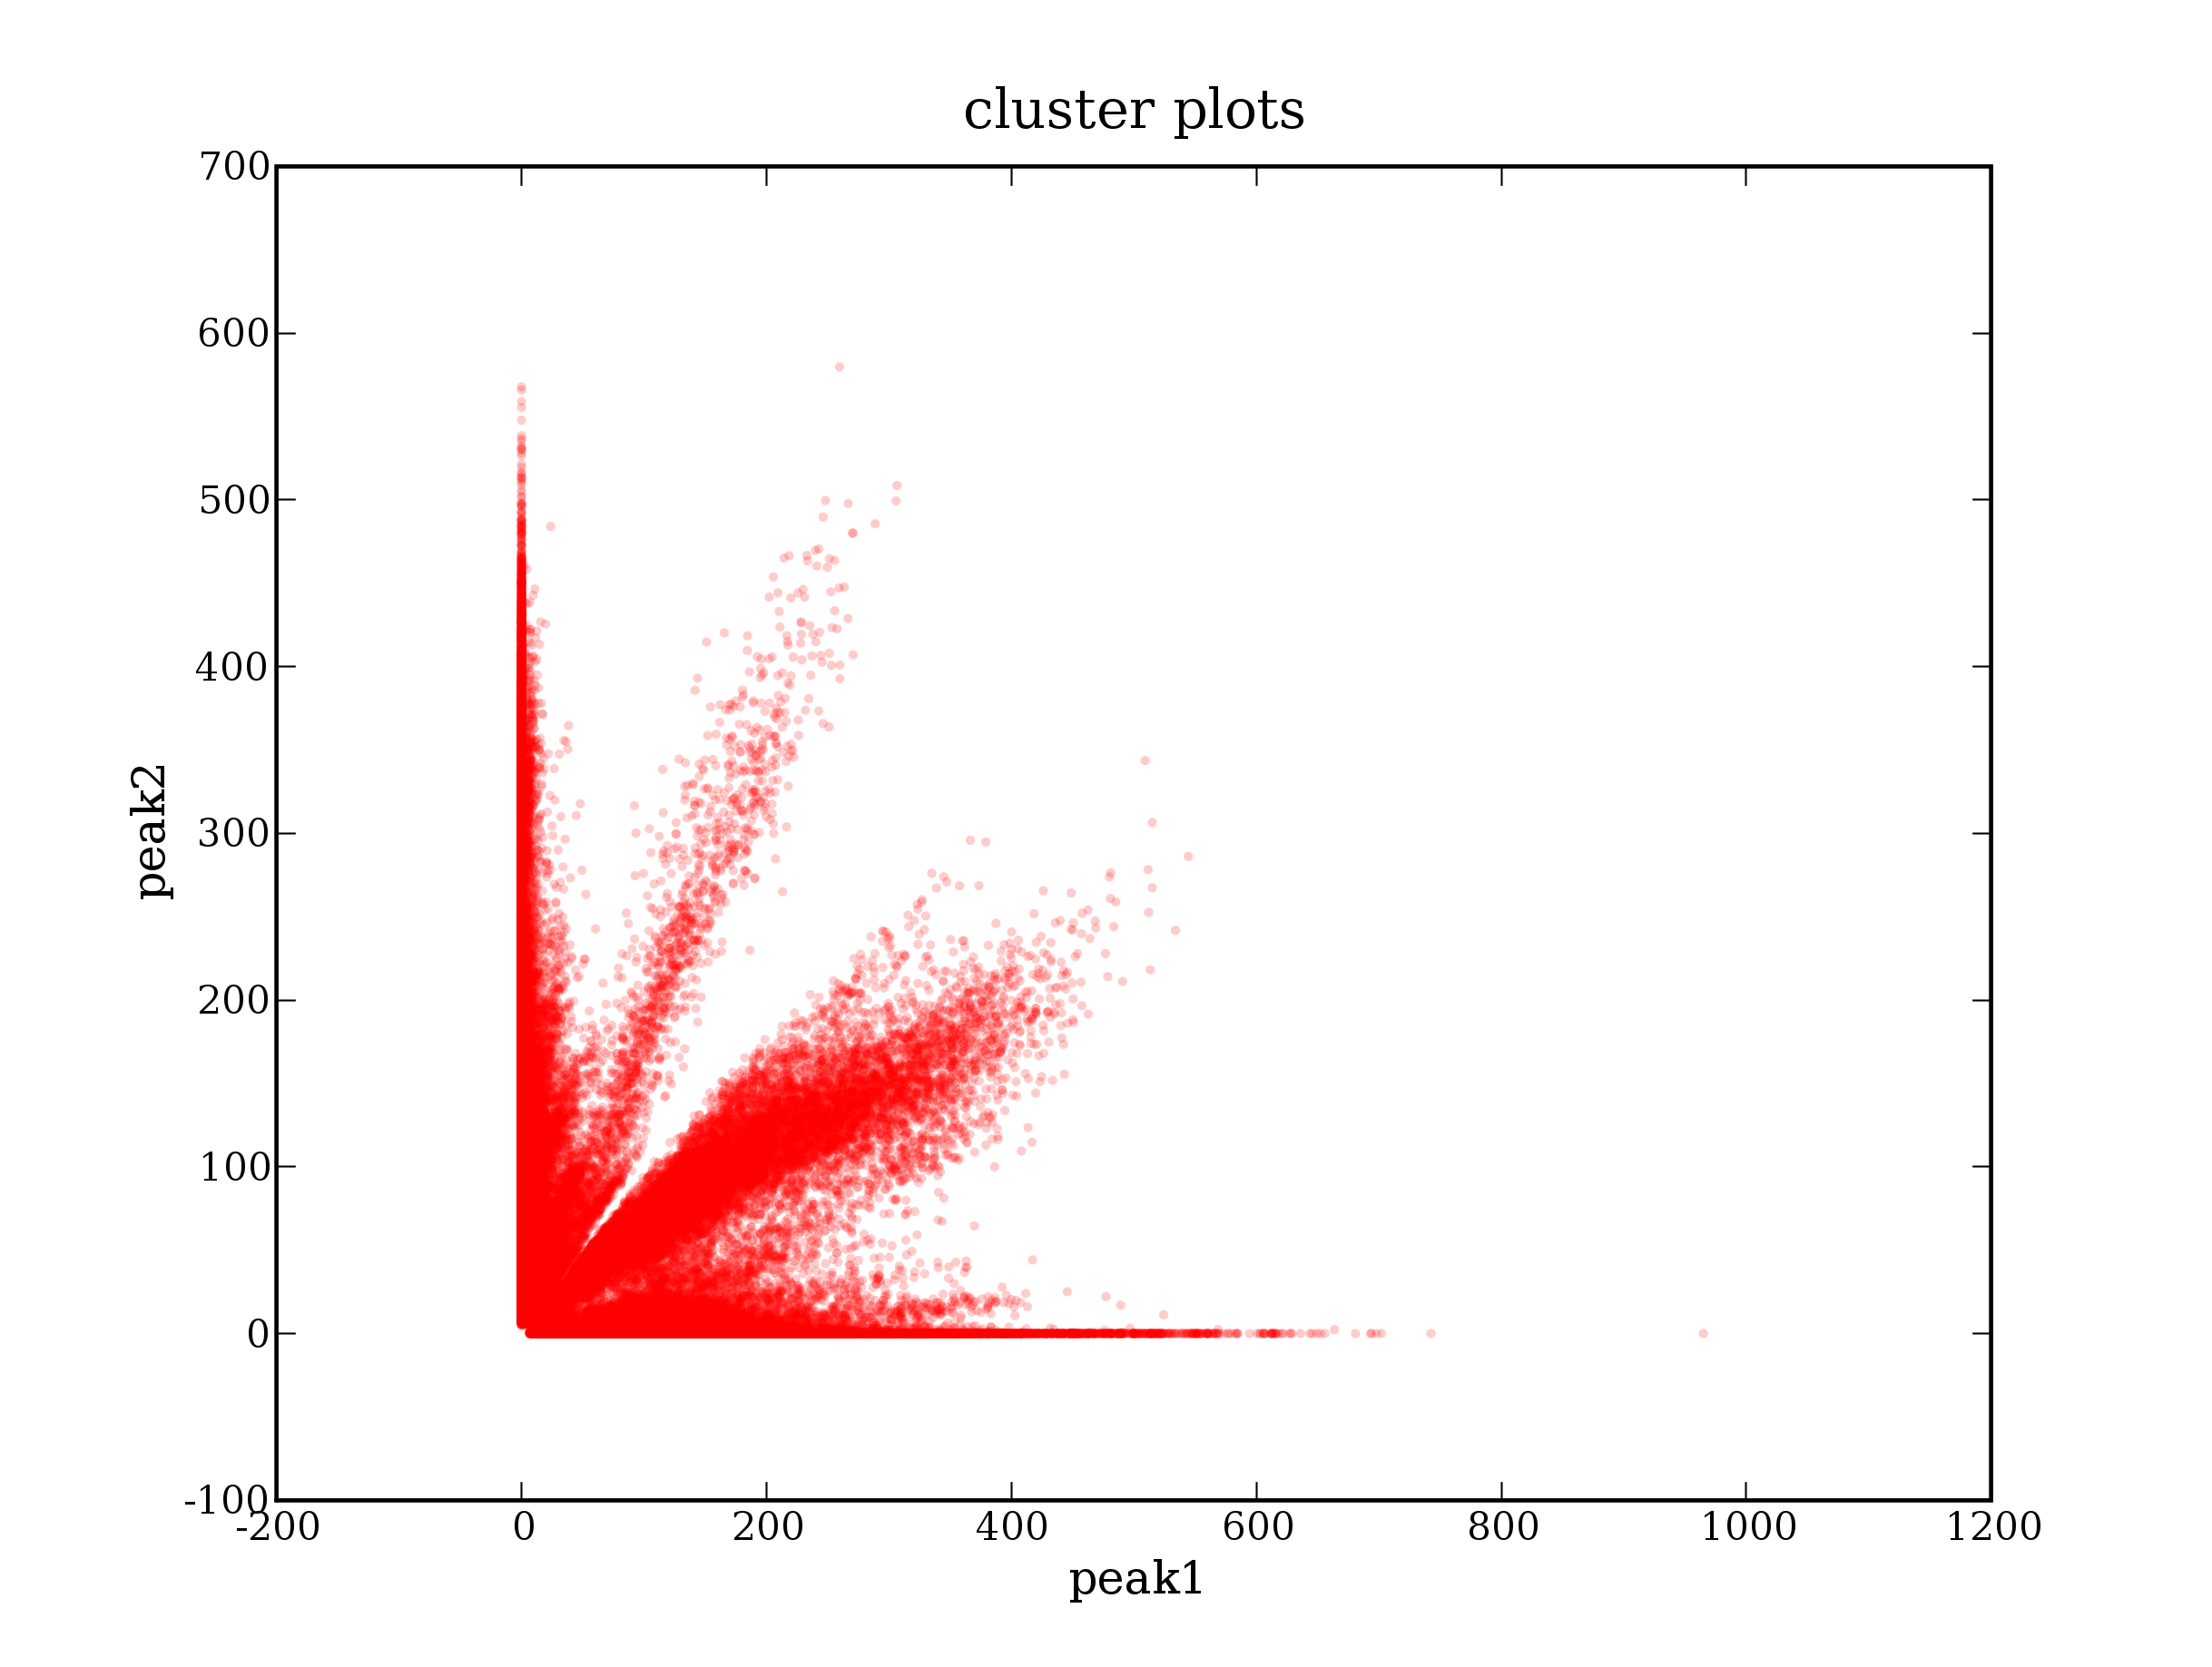
\includegraphics[width=1\textwidth]{figures/cluster_plots_allele1.png}
\caption{homozygote for allele 1}\label{f1}
\end{figure}

\begin{figure}
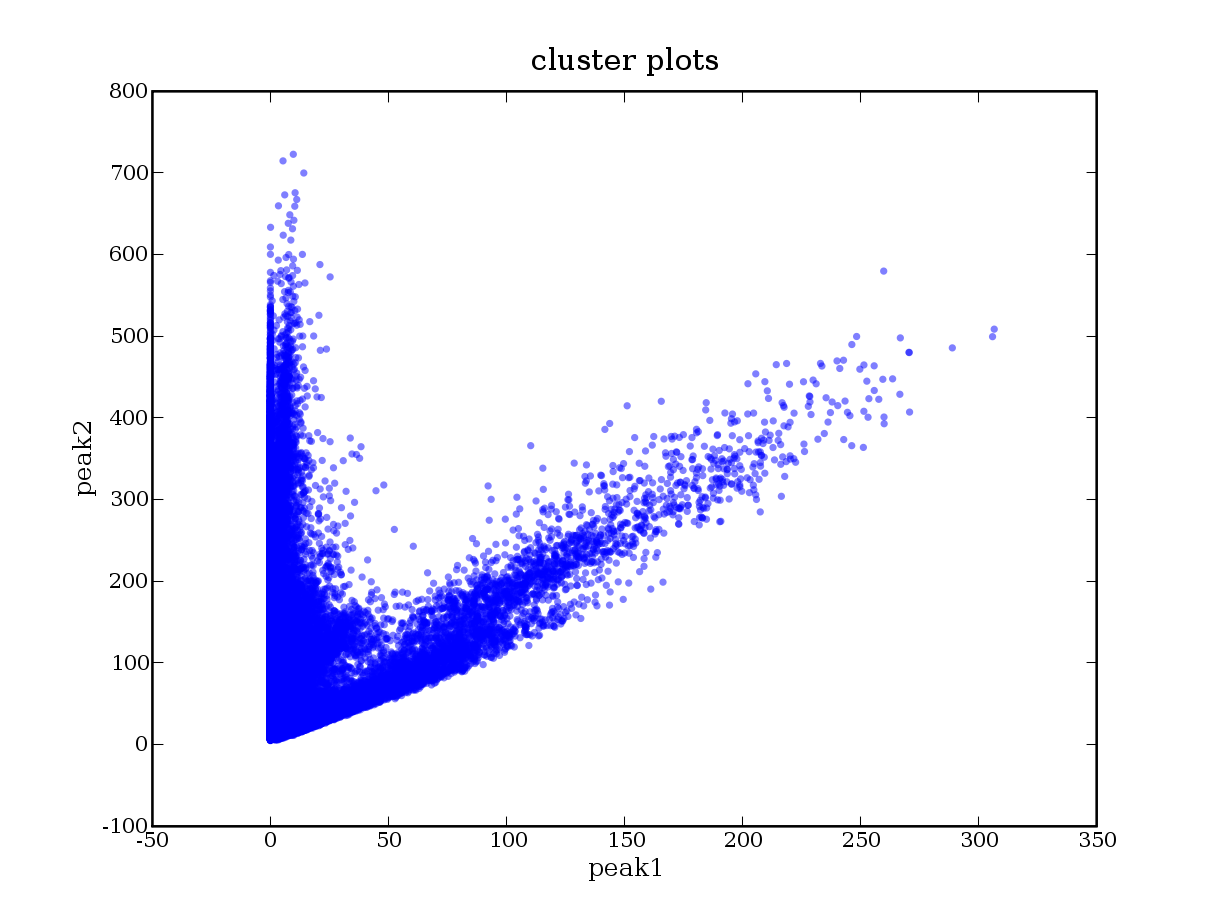
\includegraphics[width=1\textwidth]{figures/cluster_plots_allele2.png}
\caption{homozygote for allele 2}\label{f2}
\end{figure}

\begin{figure}
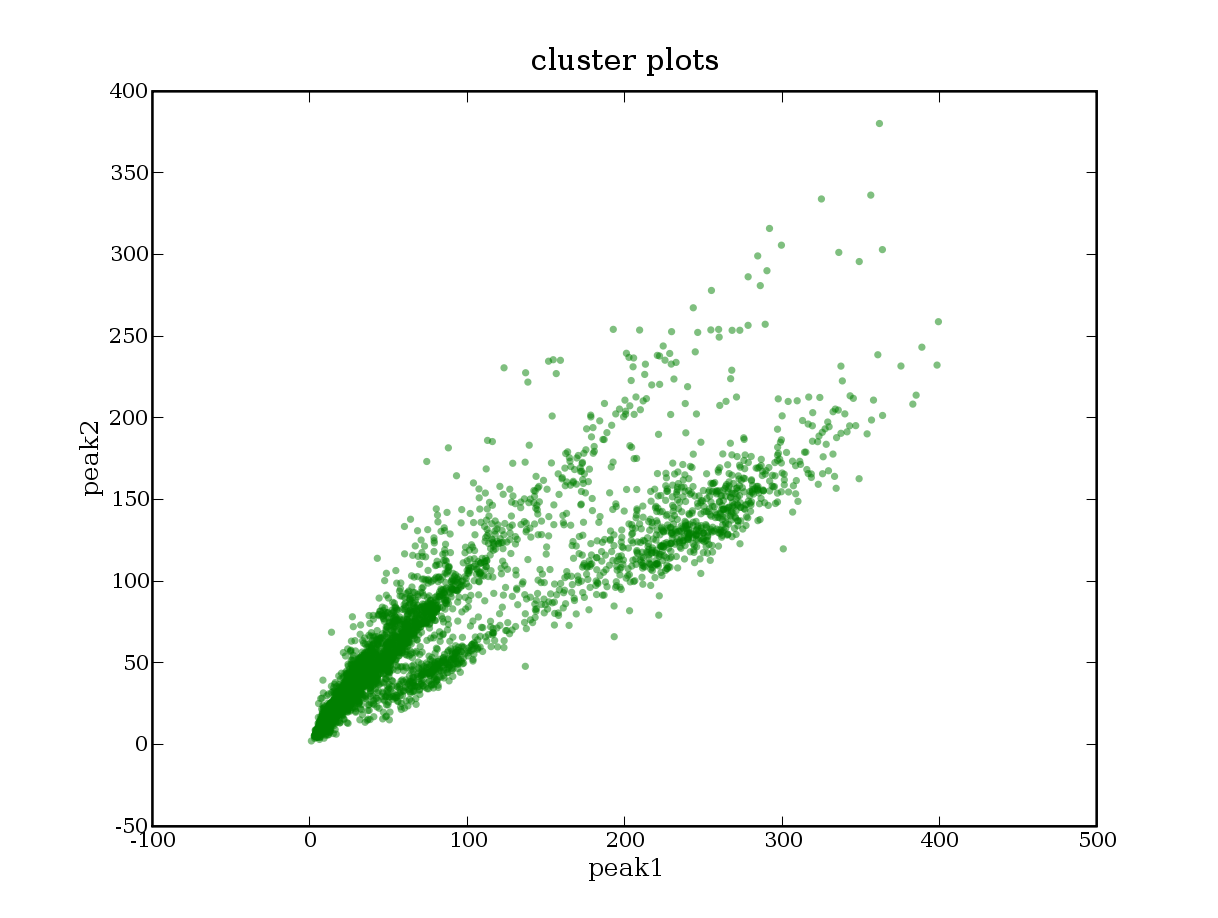
\includegraphics[width=1\textwidth]{figures/cluster_plots_het.png}
\caption{heterozygote}\label{f3}
\end{figure}

\begin{figure}
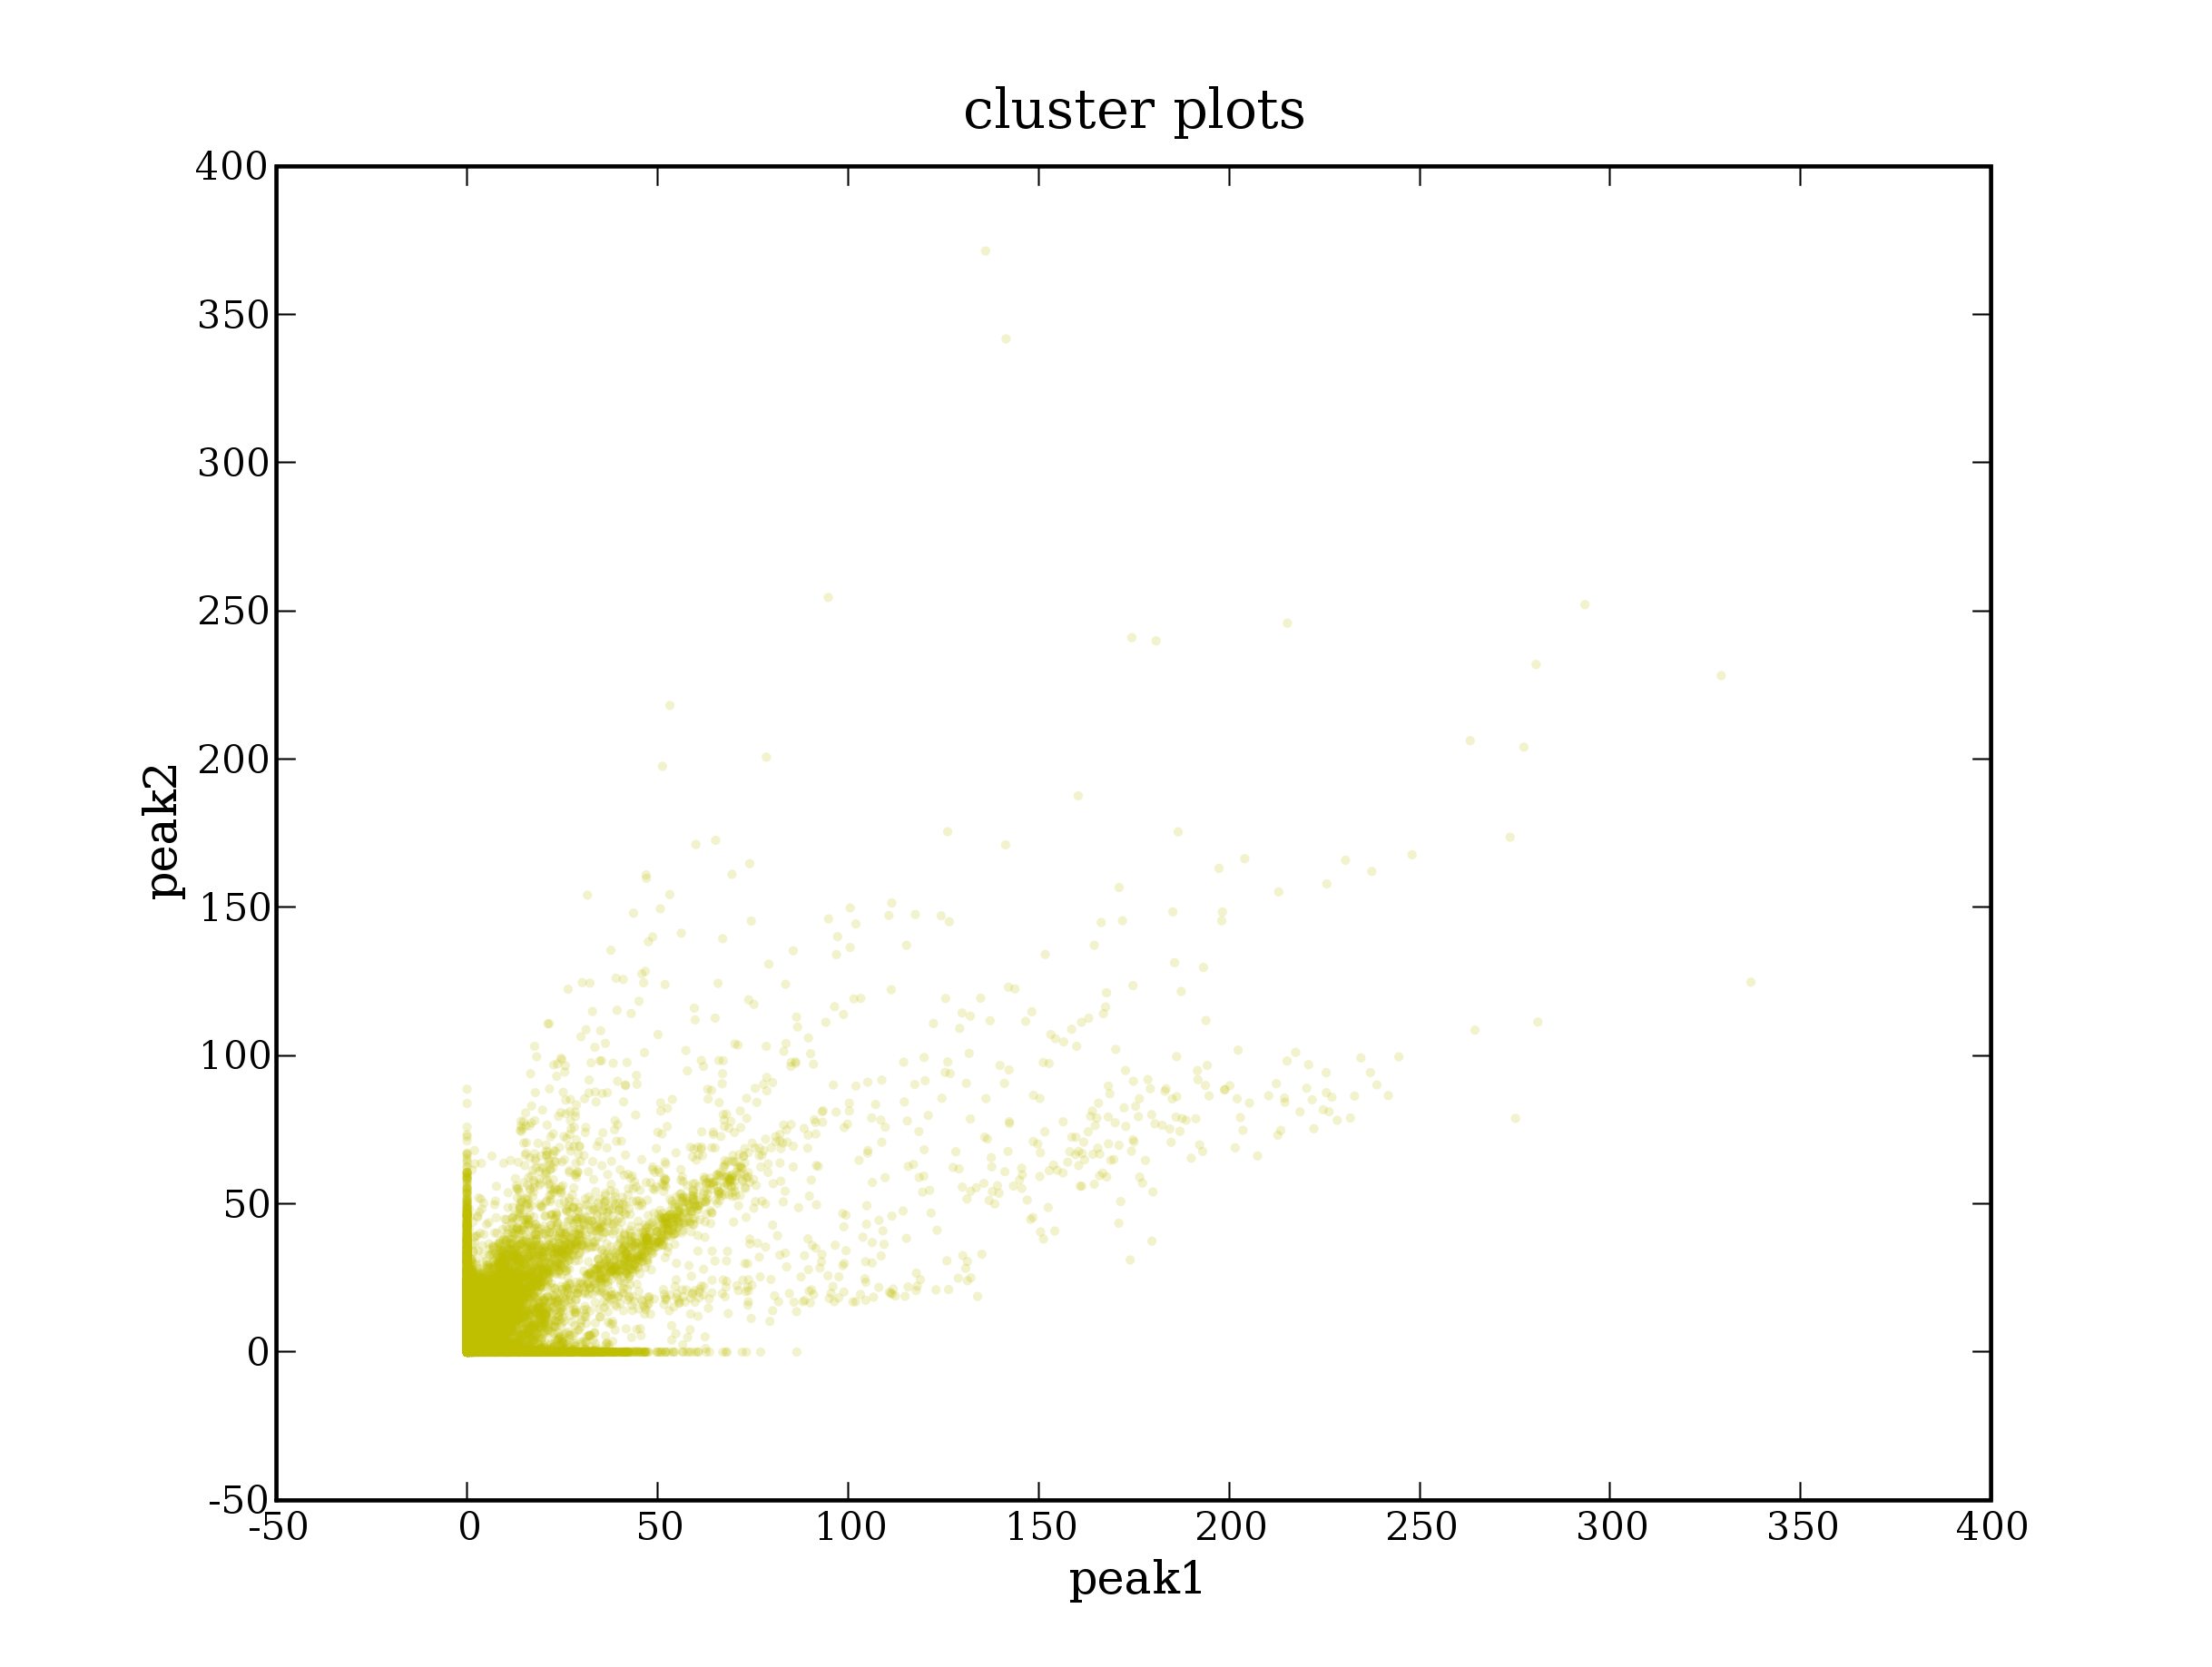
\includegraphics[width=1\textwidth]{figures/cluster_plots_NA.png}
\caption{missing/NA}\label{f4}
\end{figure}

\begin{figure}
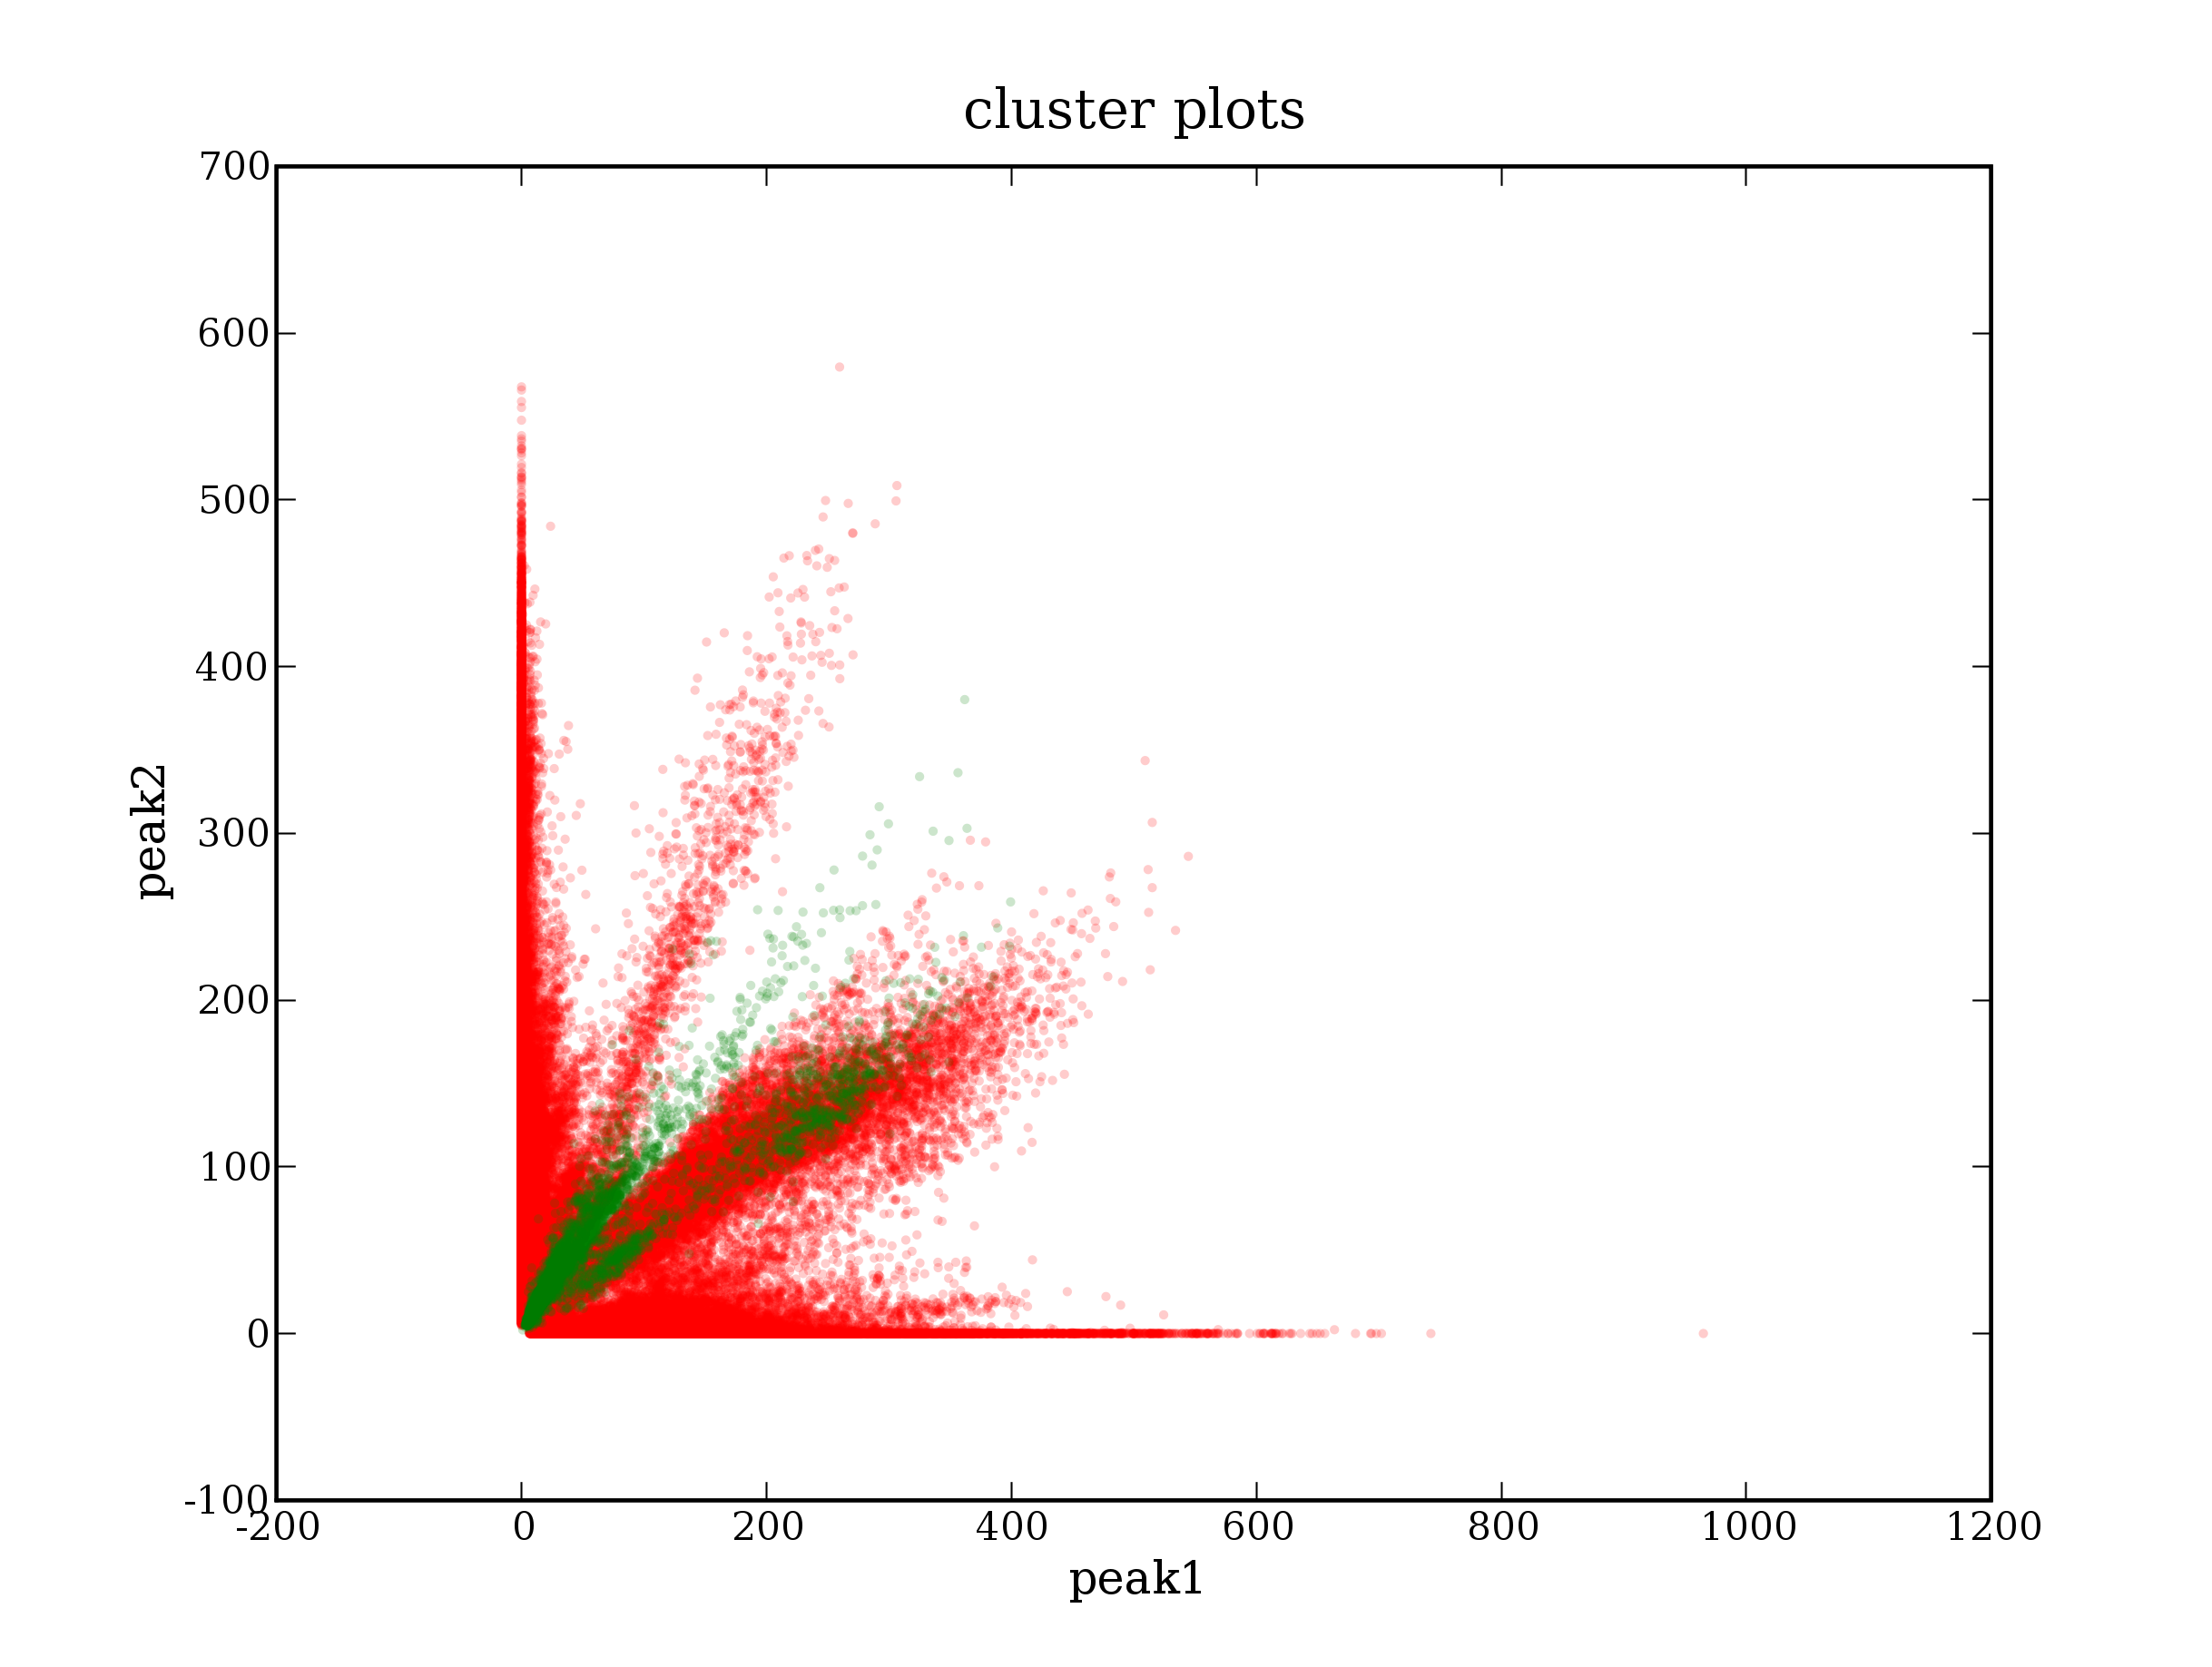
\includegraphics[width=1\textwidth]{figures/cluster_plots_allele1_het.png}
\caption{overlapping of homozygote for allele 1 and heterozygote}\label{f5}
\end{figure}

\begin{figure}
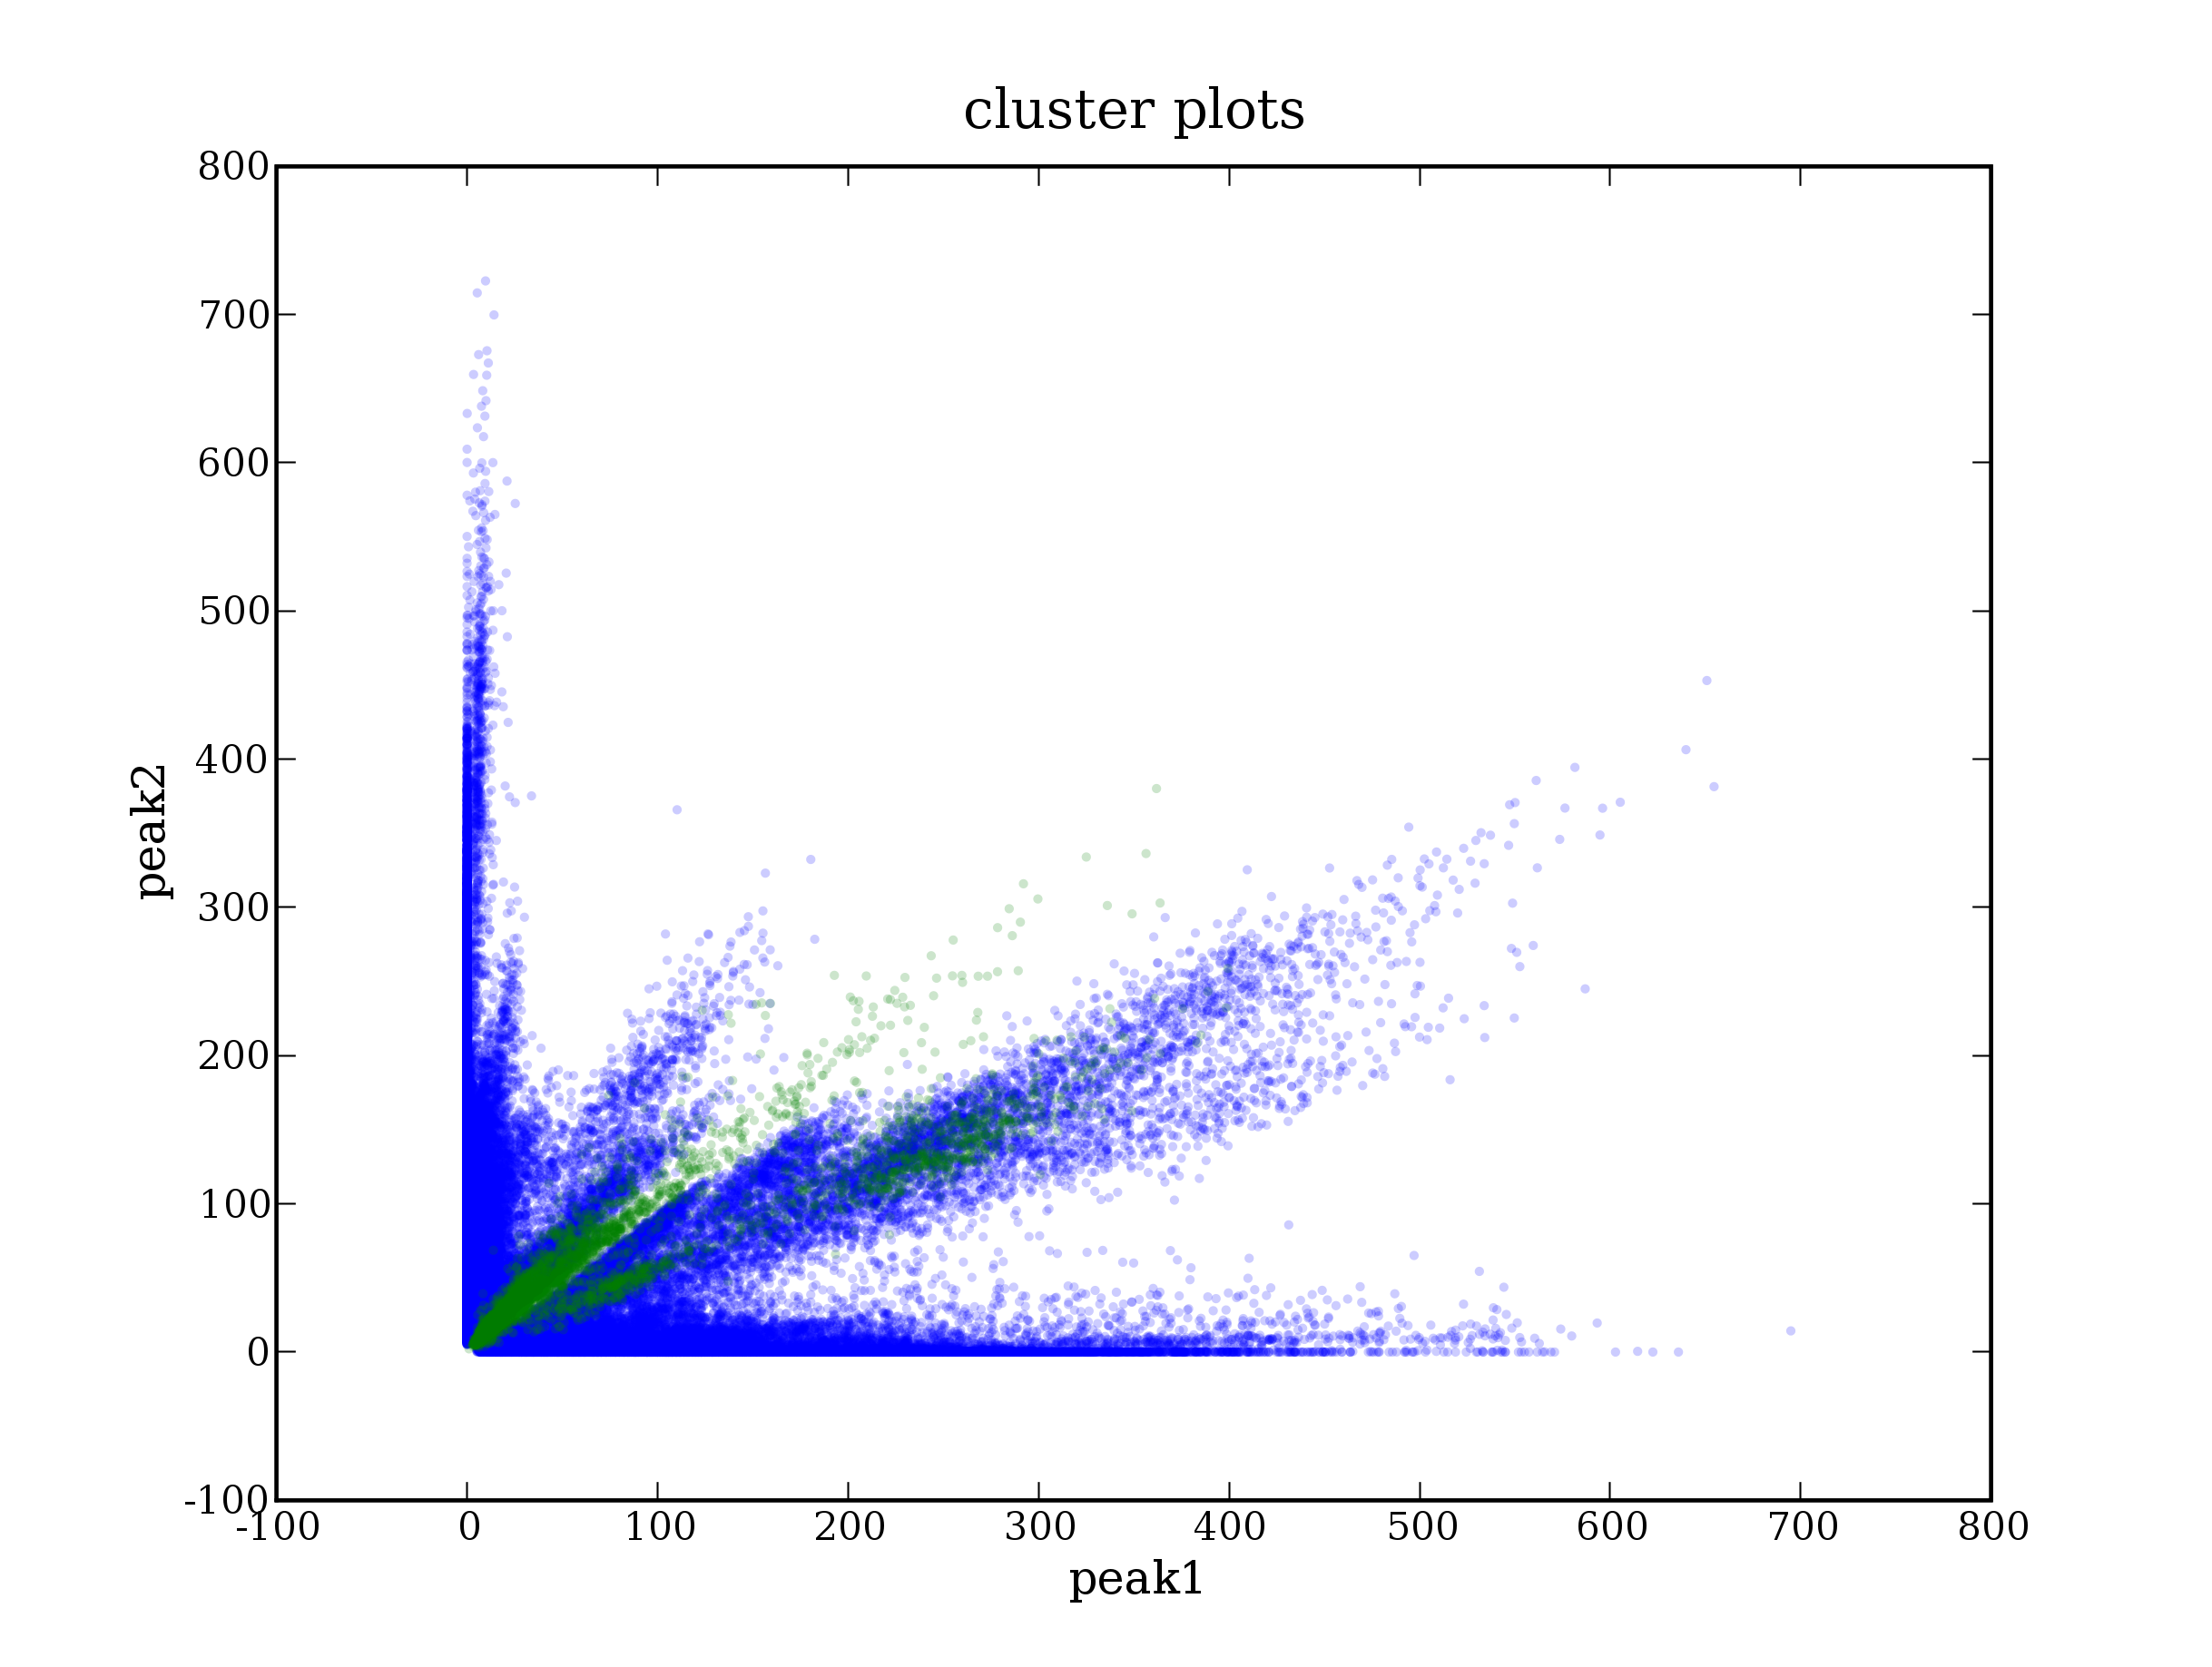
\includegraphics[width=1\textwidth]{figures/cluster_plots_allele2_het.png}
\caption{overlapping of homozygote for allele 2 and heterozygote}\label{f6}
\end{figure}

\begin{figure}
\includegraphics[width=1\textwidth]{figures/cluster_plots_allele1_allele2.png}
\caption{overlapping of homozygote for allele 1 and allele 2}\label{f7}
\end{figure}

\begin{figure}
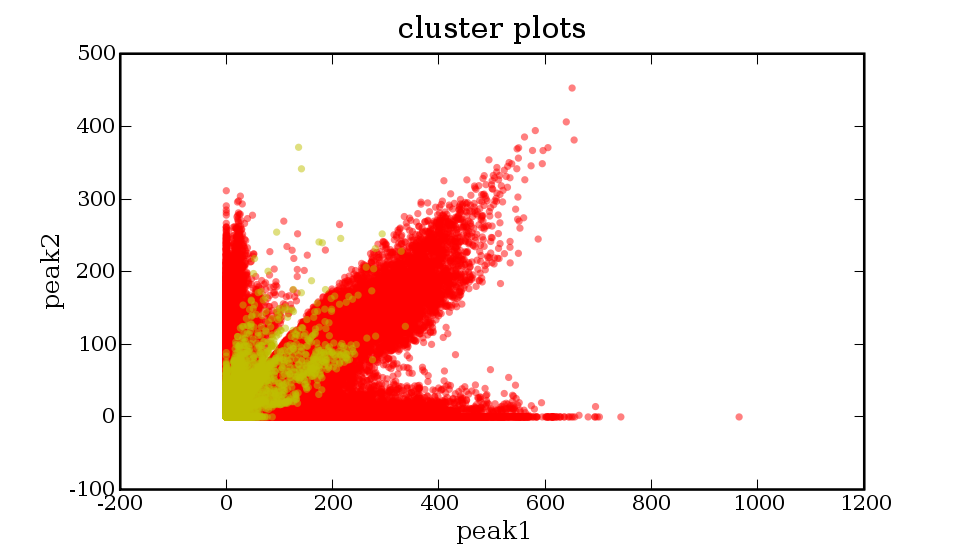
\includegraphics[width=1\textwidth]{figures/cluster_plots_allele1_NA.png}
\caption{overlapping of homozygote for allele 1 and NA}\label{f8}
\end{figure}

\begin{figure}
\includegraphics[width=1\textwidth]{figures/cluster_plots_homo_and_hetero.png}
\caption{homozygote and heterozygote}\label{f9}
\end{figure}


\begin{figure}
\includegraphics[width=1\textwidth]{figures/cluster_plots_all.png}
\caption{all four different calls}\label{f10}
\end{figure}

\subsection{cluster plots for single snp}

\begin{figure}[H]
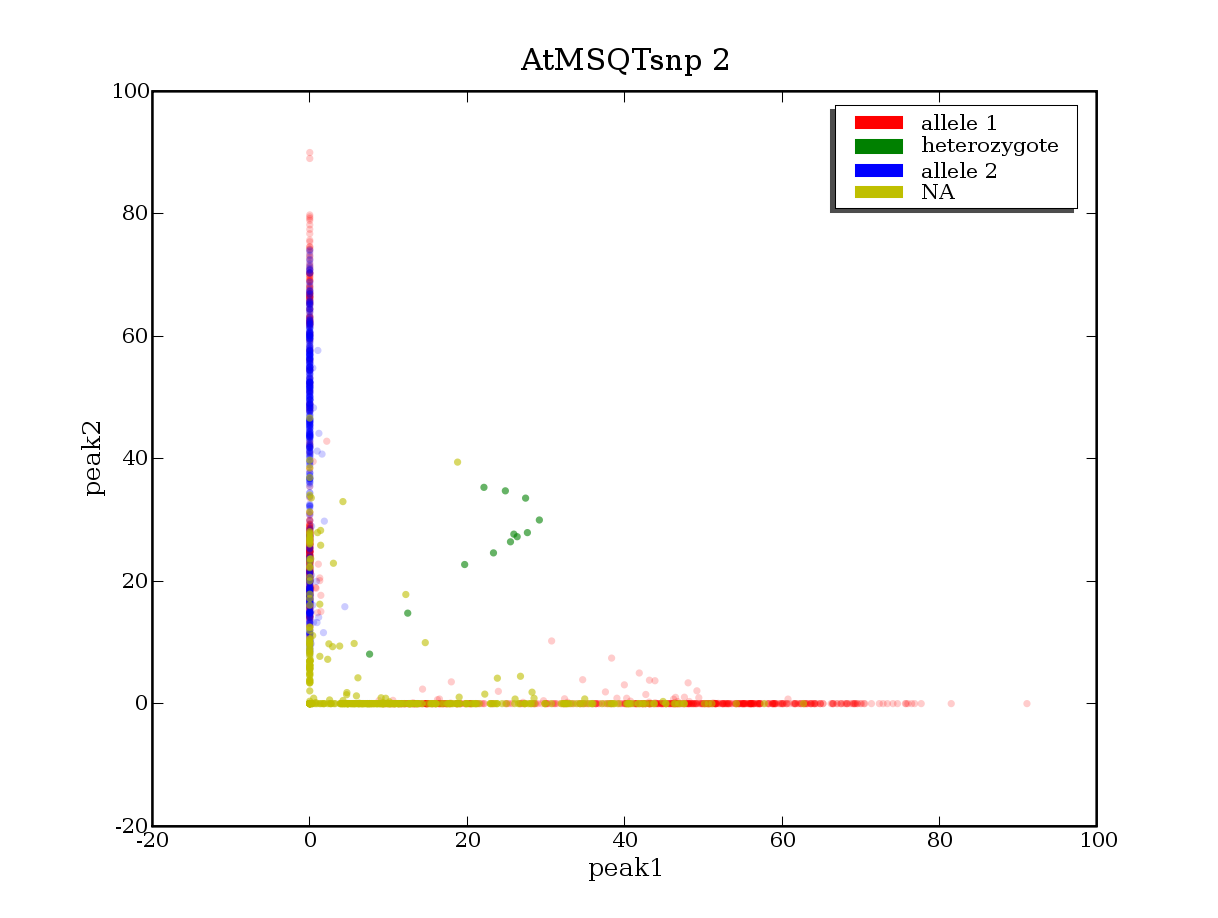
\includegraphics[width=0.5\textwidth]{figures/cluster_plot_AtMSQTsnp_2.png}
\caption{cluster plot for AtMSQTsnp 2.} \label{flAtMSQTsnp2}
\end{figure}
\begin{figure}[H]
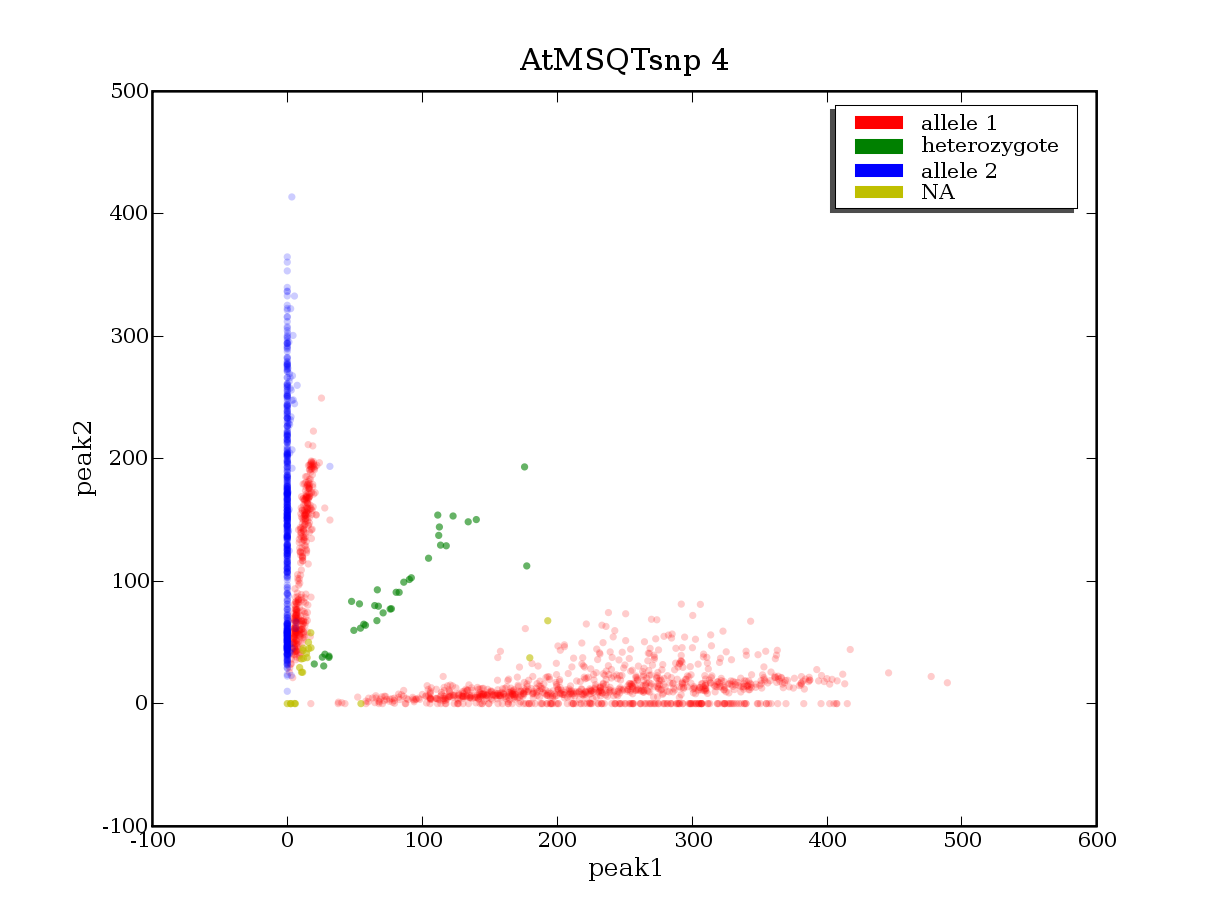
\includegraphics[width=0.5\textwidth]{figures/cluster_plot_AtMSQTsnp_4.png}
\caption{cluster plot for AtMSQTsnp 4.} \label{flAtMSQTsnp4}
\end{figure}
\begin{figure}[H]
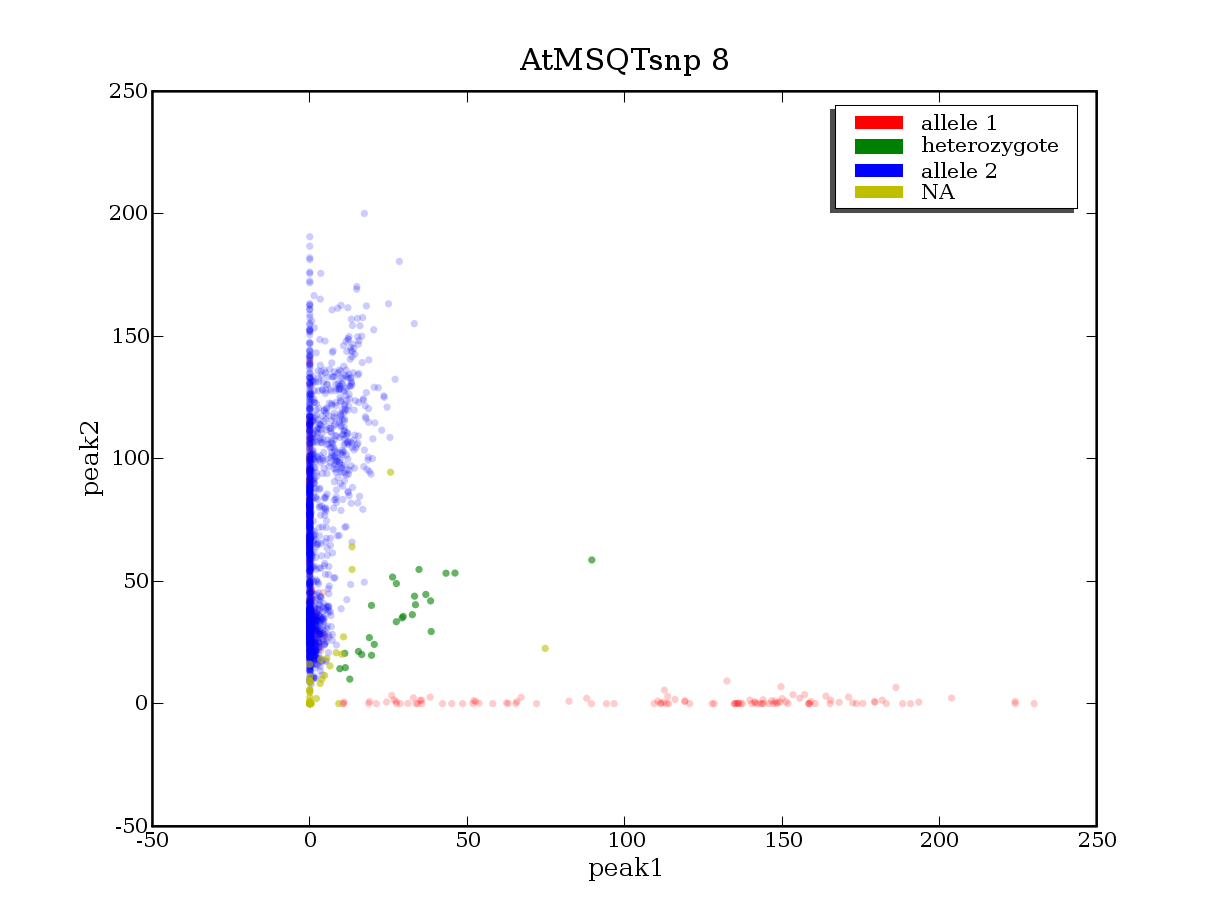
\includegraphics[width=0.5\textwidth]{figures/cluster_plot_AtMSQTsnp_8.png}
\caption{cluster plot for AtMSQTsnp 8.} \label{flAtMSQTsnp8}
\end{figure}
\begin{figure}[H]
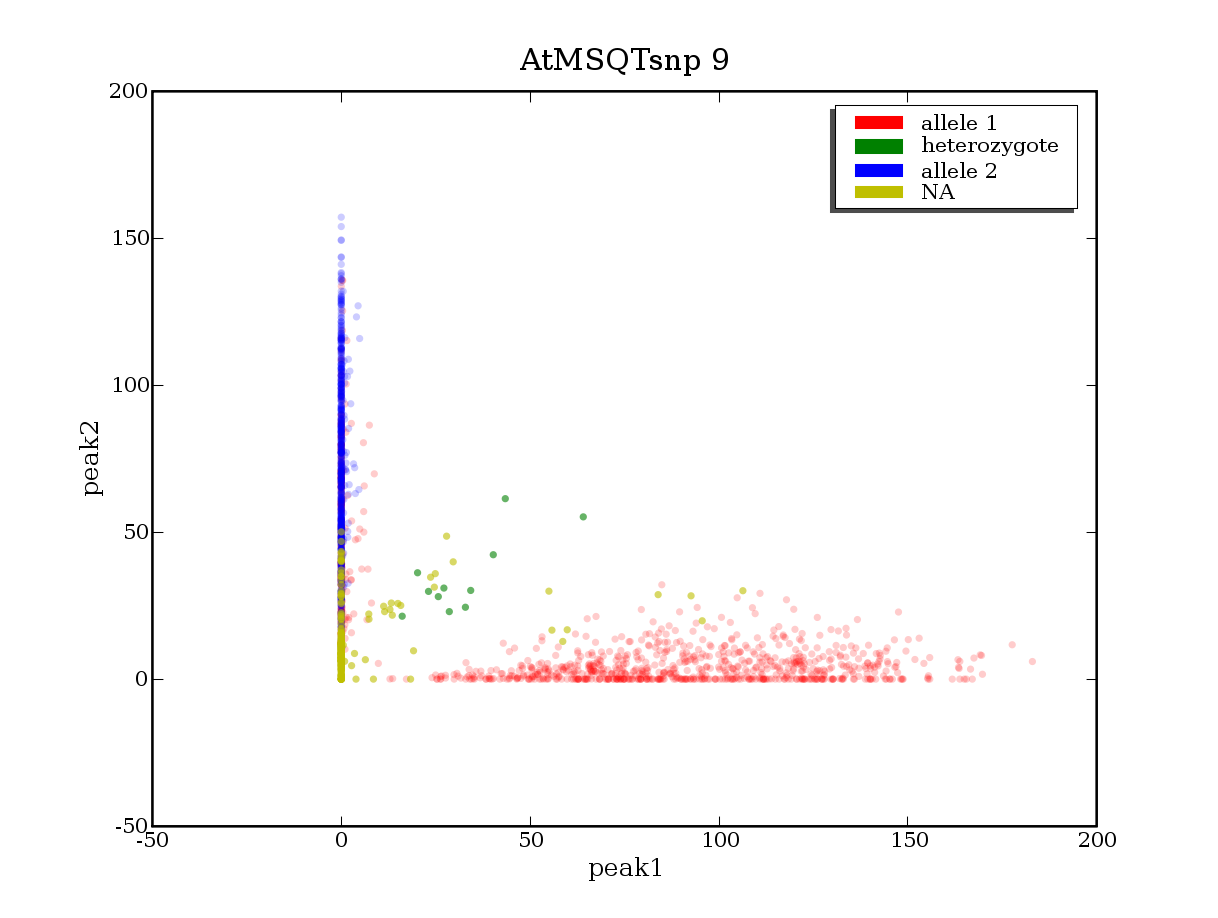
\includegraphics[width=0.5\textwidth]{figures/cluster_plot_AtMSQTsnp_9.png}
\caption{cluster plot for AtMSQTsnp 9.} \label{flAtMSQTsnp9}
\end{figure}
\begin{figure}[H]
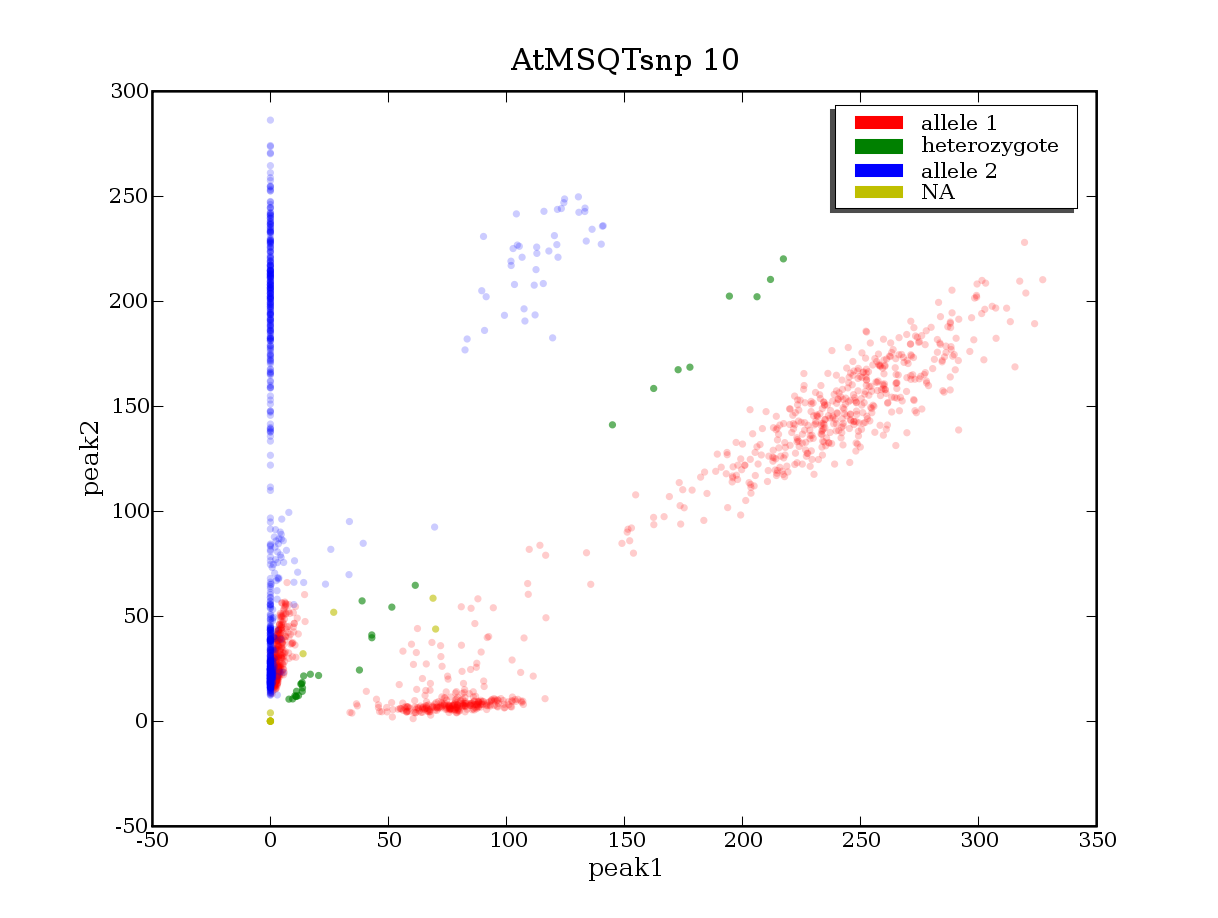
\includegraphics[width=0.5\textwidth]{figures/cluster_plot_AtMSQTsnp_10.png}
\caption{cluster plot for AtMSQTsnp 10.} \label{flAtMSQTsnp10}
\end{figure}
\begin{figure}[H]
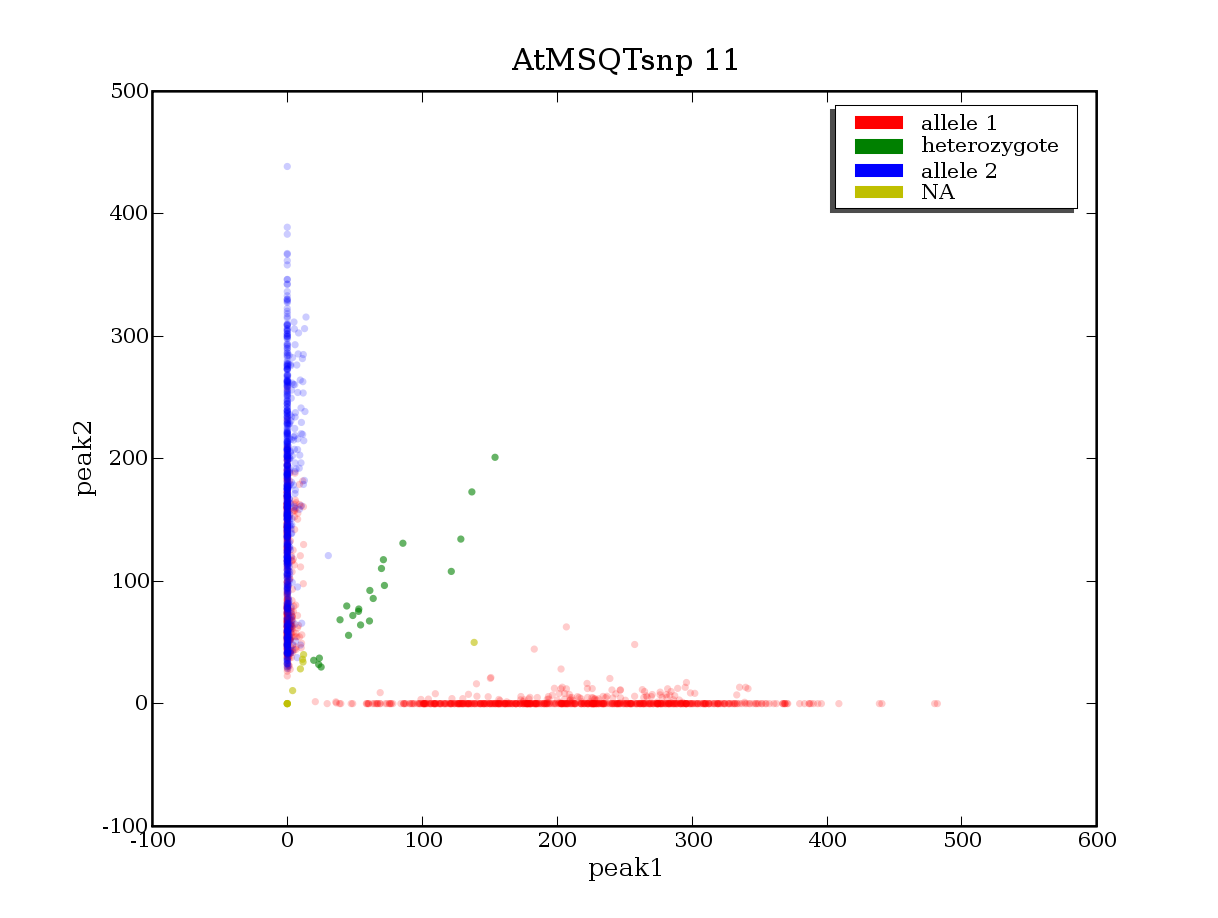
\includegraphics[width=0.5\textwidth]{figures/cluster_plot_AtMSQTsnp_11.png}
\caption{cluster plot for AtMSQTsnp 11.} \label{flAtMSQTsnp11}
\end{figure}
\begin{figure}[H]
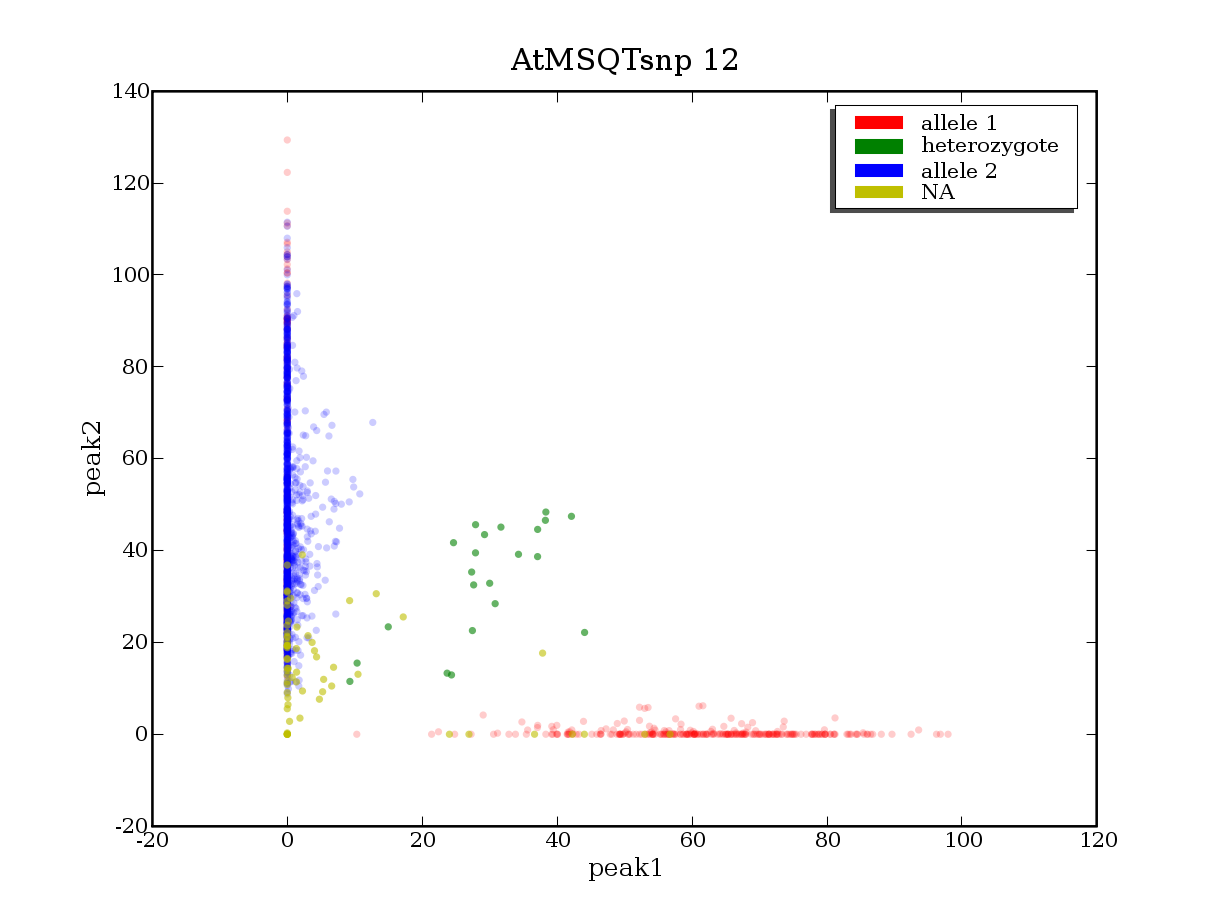
\includegraphics[width=0.5\textwidth]{figures/cluster_plot_AtMSQTsnp_12.png}
\caption{cluster plot for AtMSQTsnp 12.} \label{flAtMSQTsnp12}
\end{figure}
\begin{figure}[H]
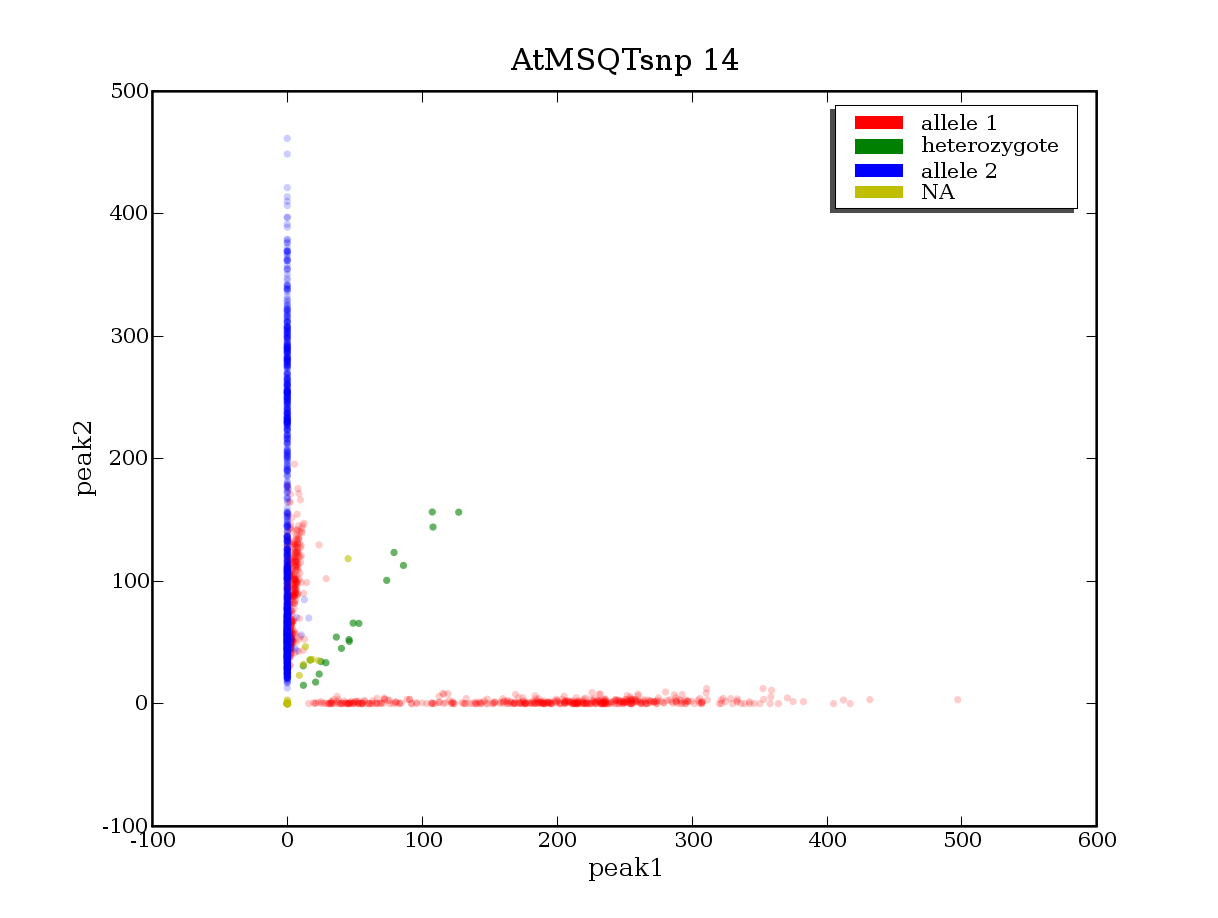
\includegraphics[width=0.5\textwidth]{figures/cluster_plot_AtMSQTsnp_14.png}
\caption{cluster plot for AtMSQTsnp 14.} \label{flAtMSQTsnp14}
\end{figure}
\begin{figure}[H]
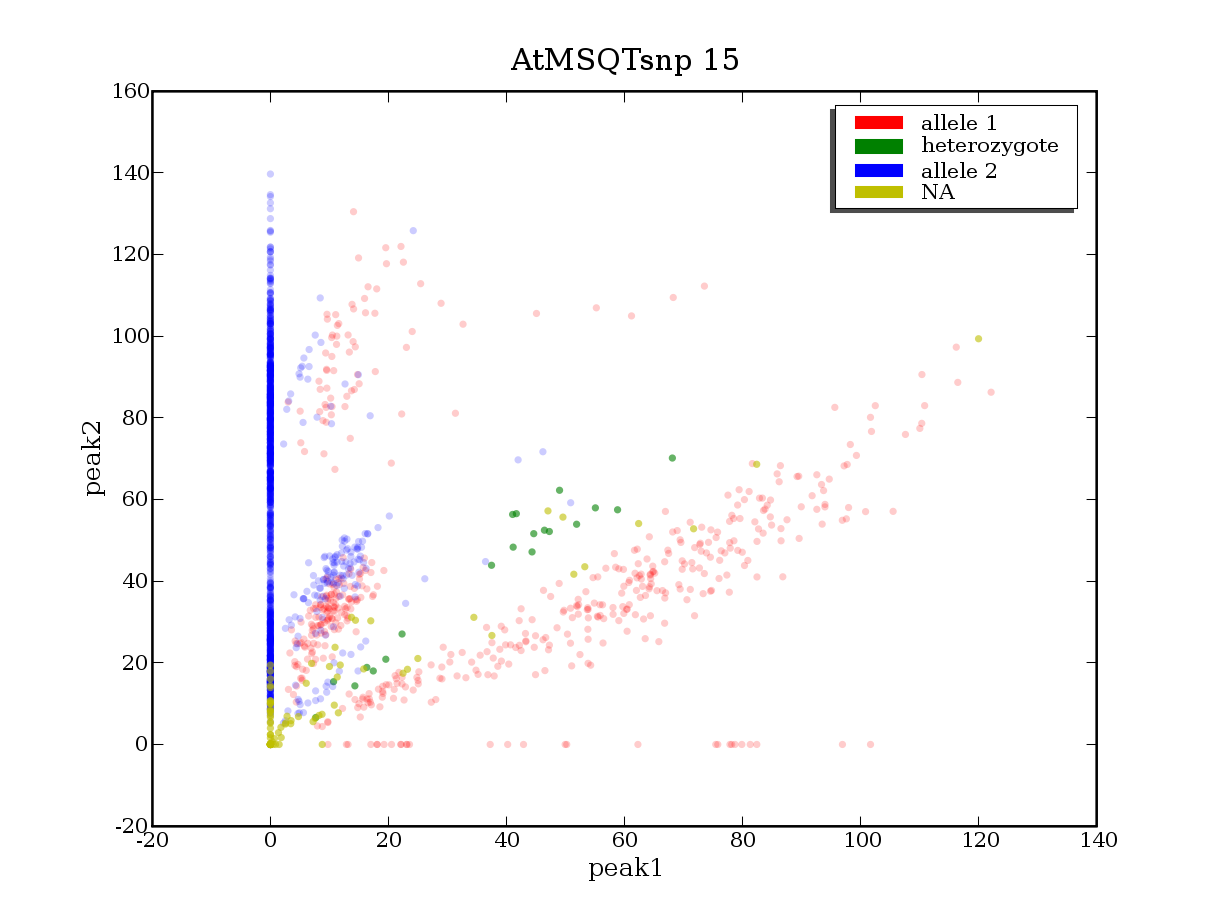
\includegraphics[width=0.5\textwidth]{figures/cluster_plot_AtMSQTsnp_15.png}
\caption{cluster plot for AtMSQTsnp 15.} \label{flAtMSQTsnp15}
\end{figure}
\begin{figure}[H]
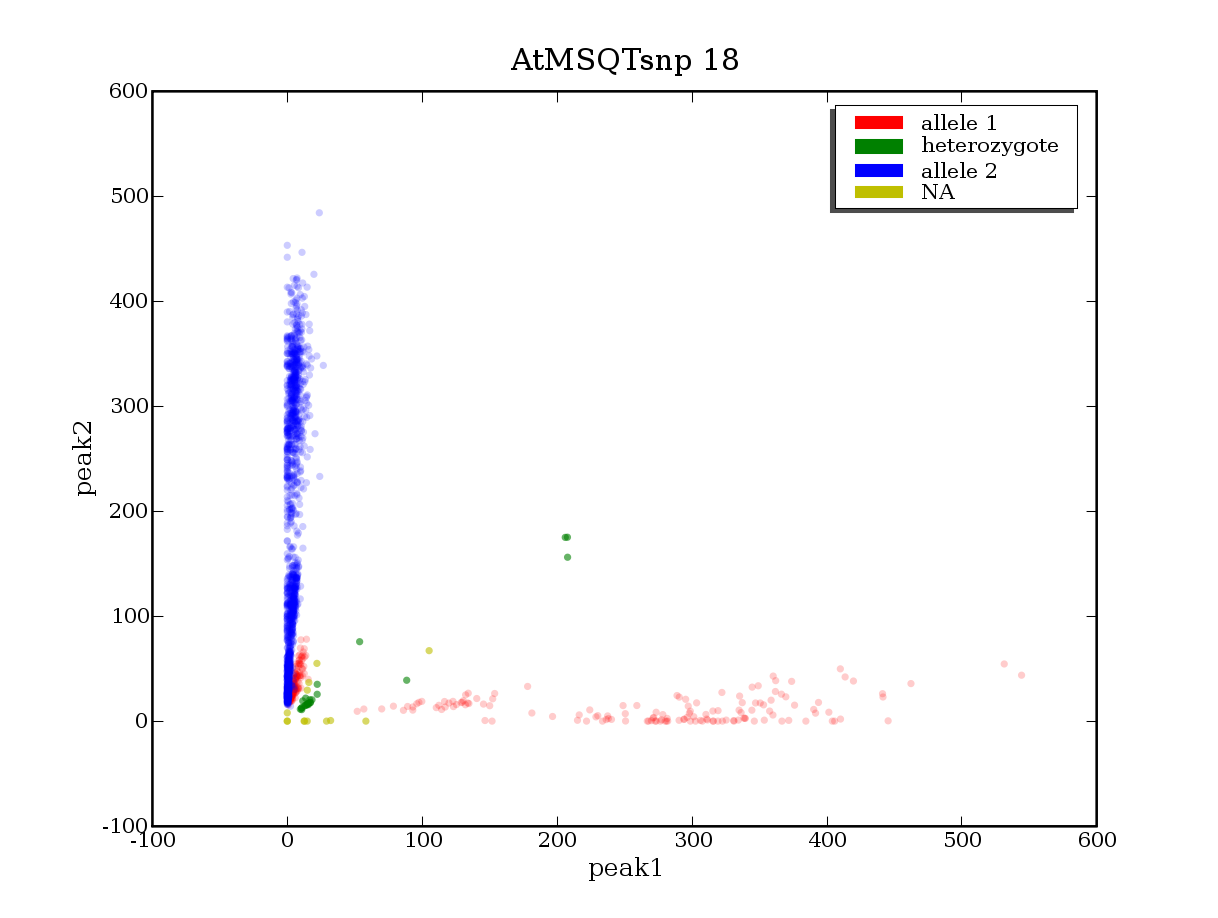
\includegraphics[width=0.5\textwidth]{figures/cluster_plot_AtMSQTsnp_18.png}
\caption{cluster plot for AtMSQTsnp 18.} \label{flAtMSQTsnp18}
\end{figure}
\begin{figure}[H]
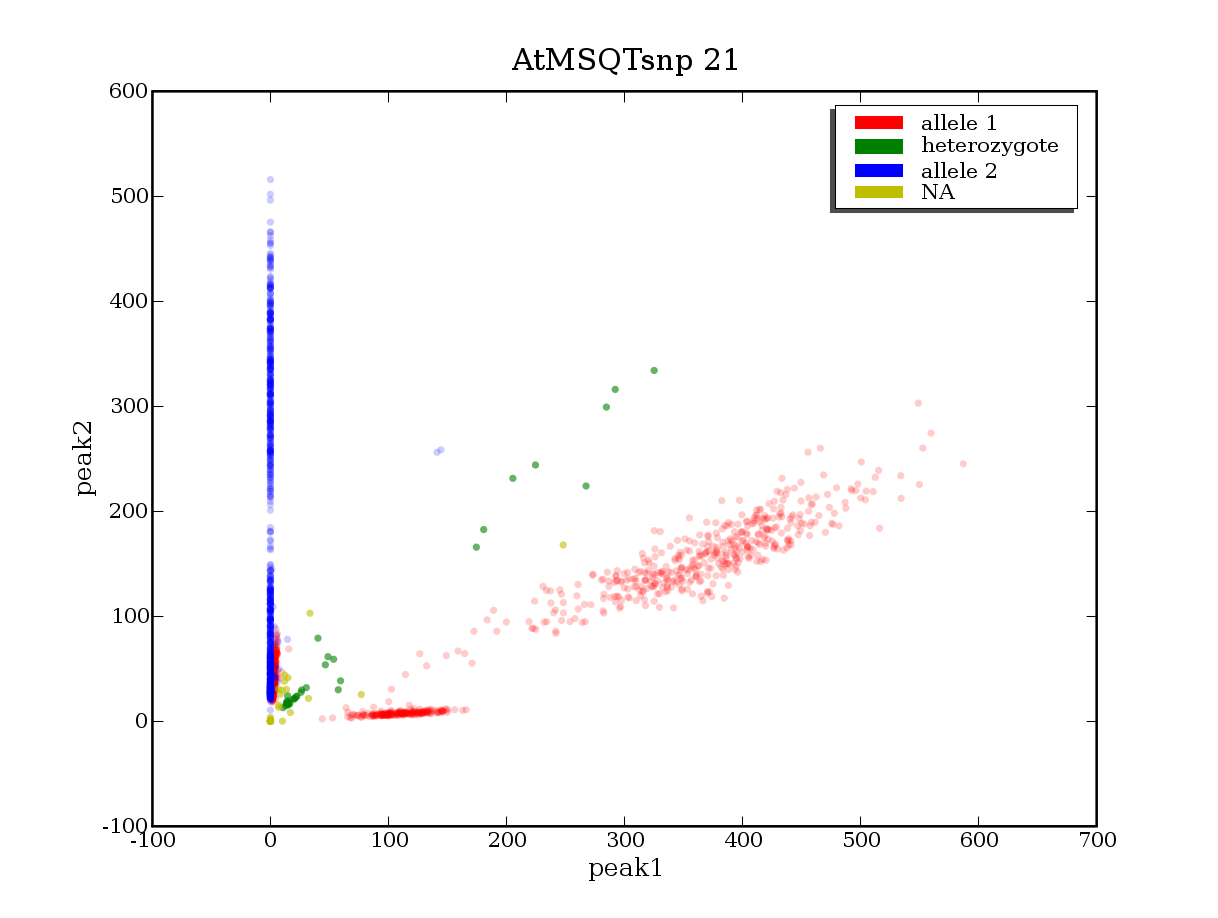
\includegraphics[width=0.5\textwidth]{figures/cluster_plot_AtMSQTsnp_21.png}
\caption{cluster plot for AtMSQTsnp 21.} \label{flAtMSQTsnp21}
\end{figure}
\begin{figure}[H]
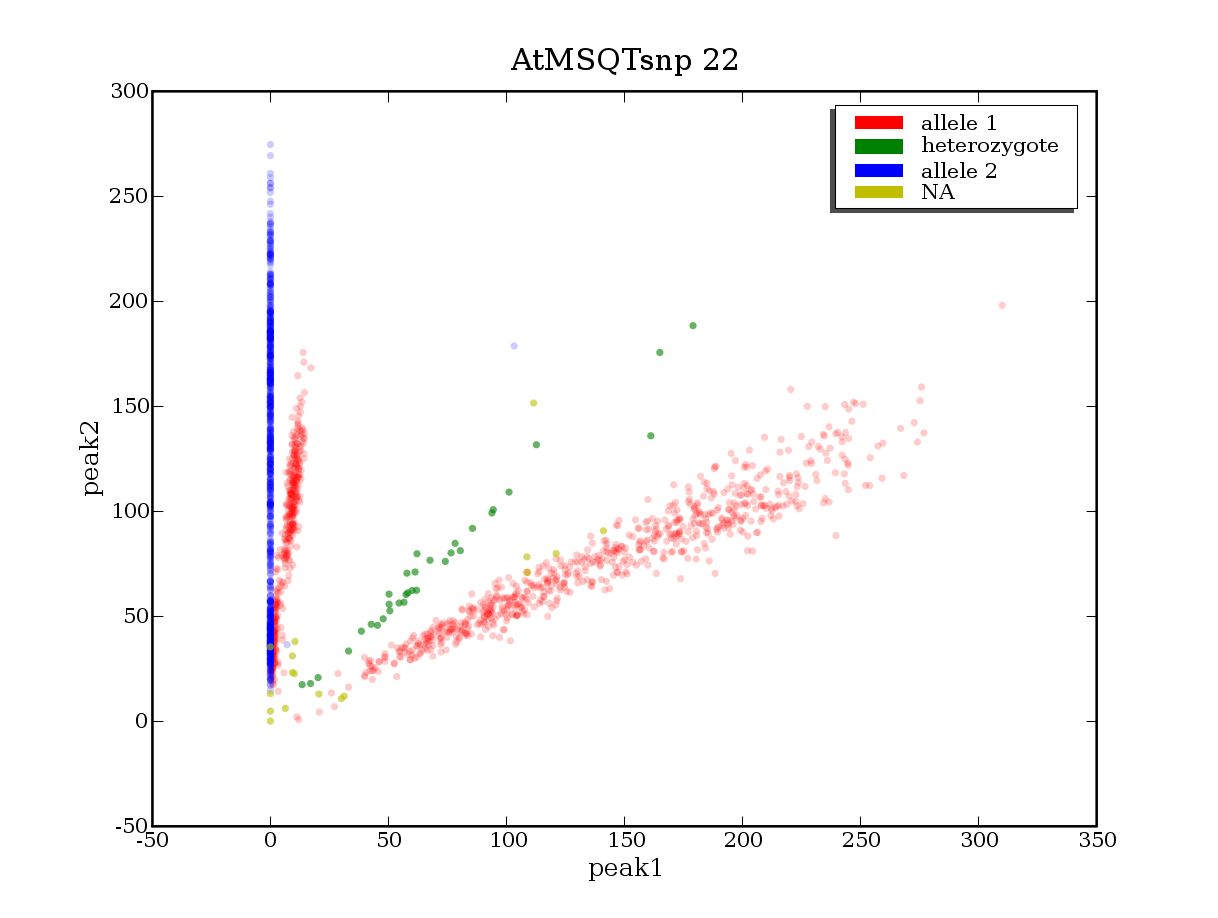
\includegraphics[width=0.5\textwidth]{figures/cluster_plot_AtMSQTsnp_22.png}
\caption{cluster plot for AtMSQTsnp 22.} \label{flAtMSQTsnp22}
\end{figure}
\begin{figure}[H]
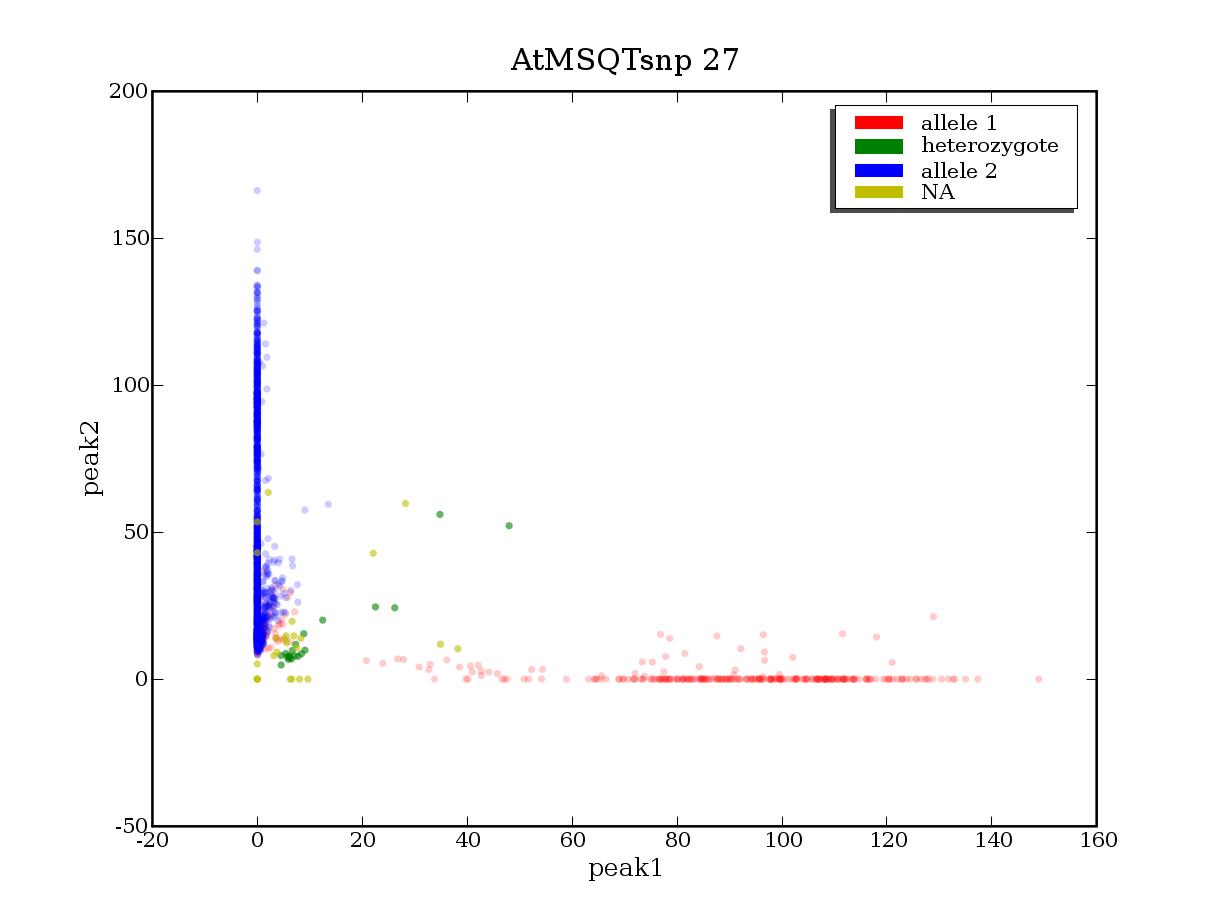
\includegraphics[width=0.5\textwidth]{figures/cluster_plot_AtMSQTsnp_27.png}
\caption{cluster plot for AtMSQTsnp 27.} \label{flAtMSQTsnp27}
\end{figure}
\begin{figure}[H]
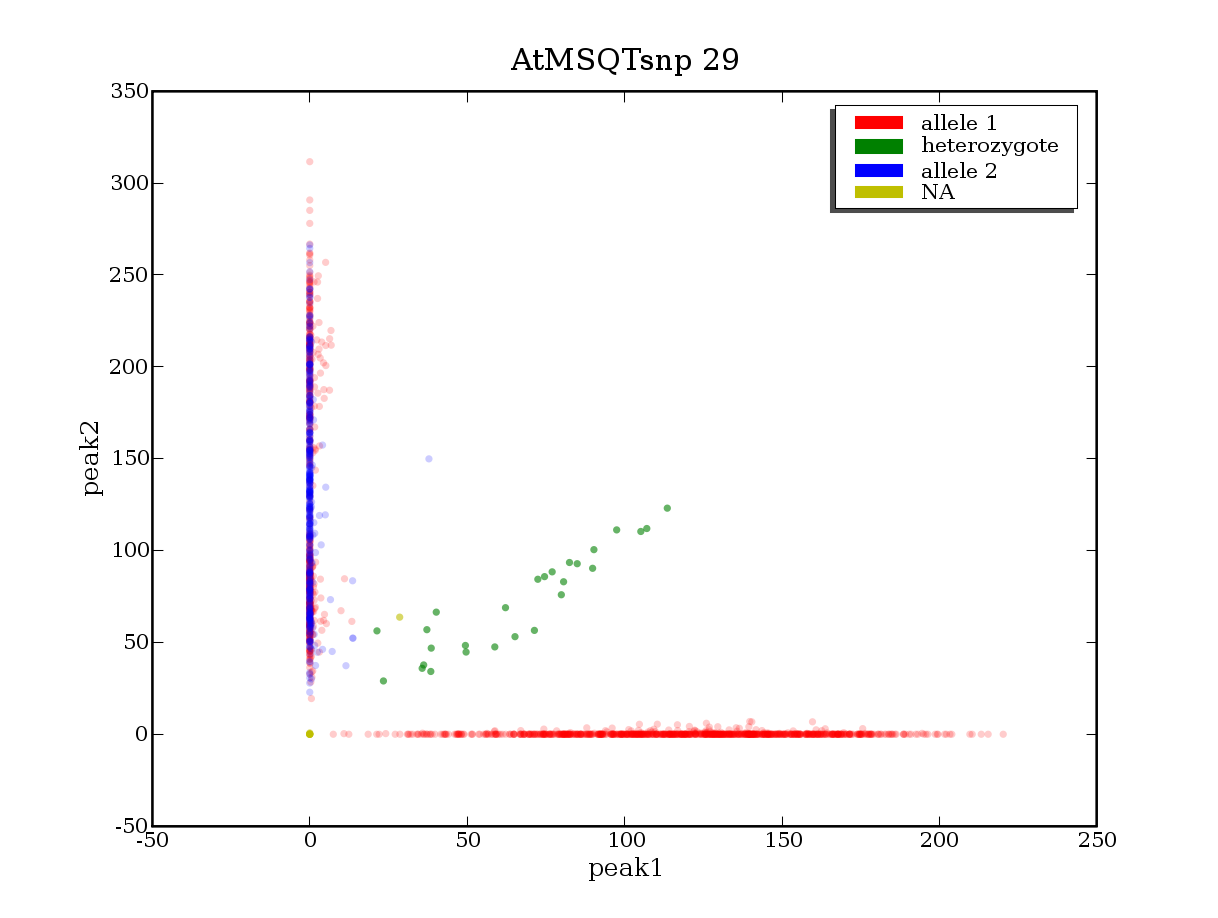
\includegraphics[width=0.5\textwidth]{figures/cluster_plot_AtMSQTsnp_29.png}
\caption{cluster plot for AtMSQTsnp 29.} \label{flAtMSQTsnp29}
\end{figure}
\begin{figure}[H]
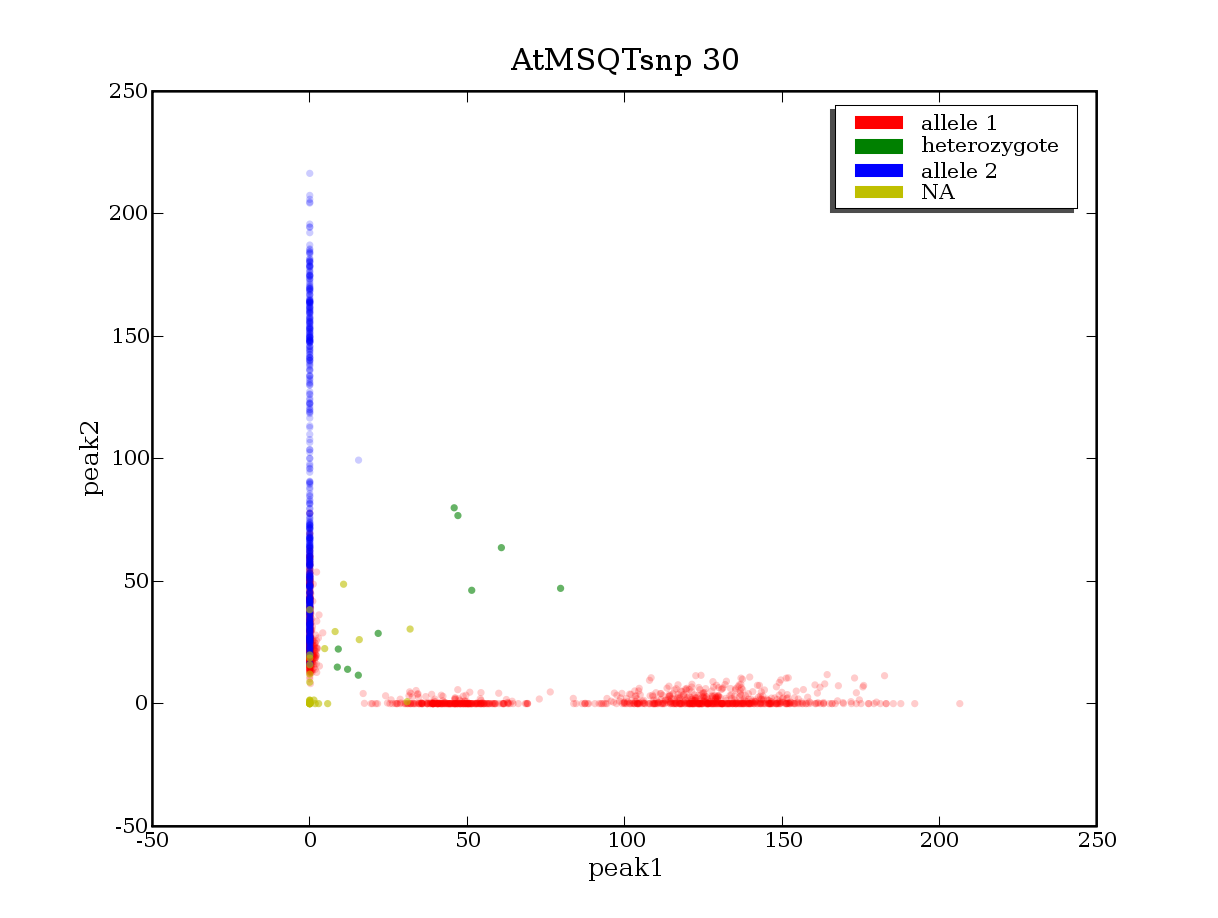
\includegraphics[width=0.5\textwidth]{figures/cluster_plot_AtMSQTsnp_30.png}
\caption{cluster plot for AtMSQTsnp 30.} \label{flAtMSQTsnp30}
\end{figure}
\begin{figure}[H]
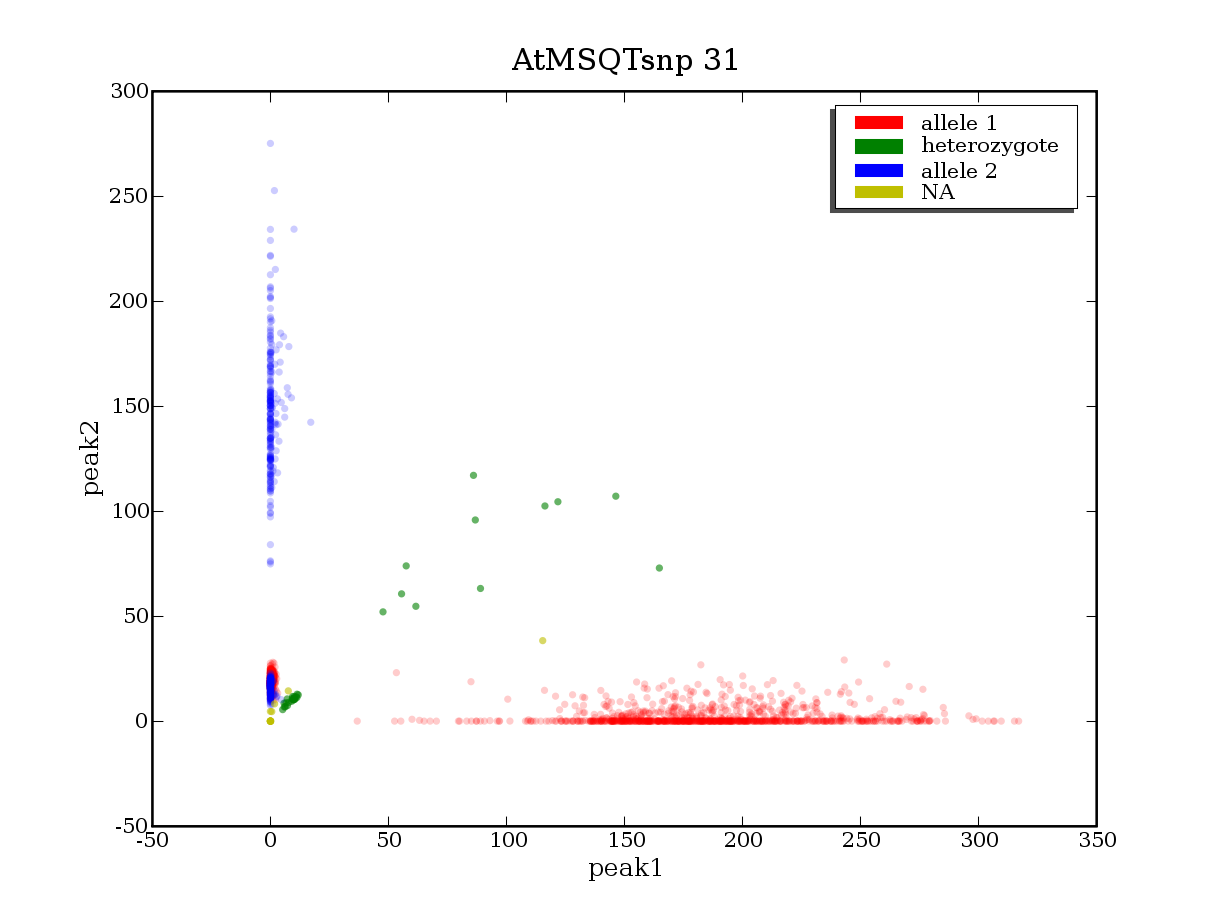
\includegraphics[width=0.5\textwidth]{figures/cluster_plot_AtMSQTsnp_31.png}
\caption{cluster plot for AtMSQTsnp 31.} \label{flAtMSQTsnp31}
\end{figure}
\begin{figure}[H]
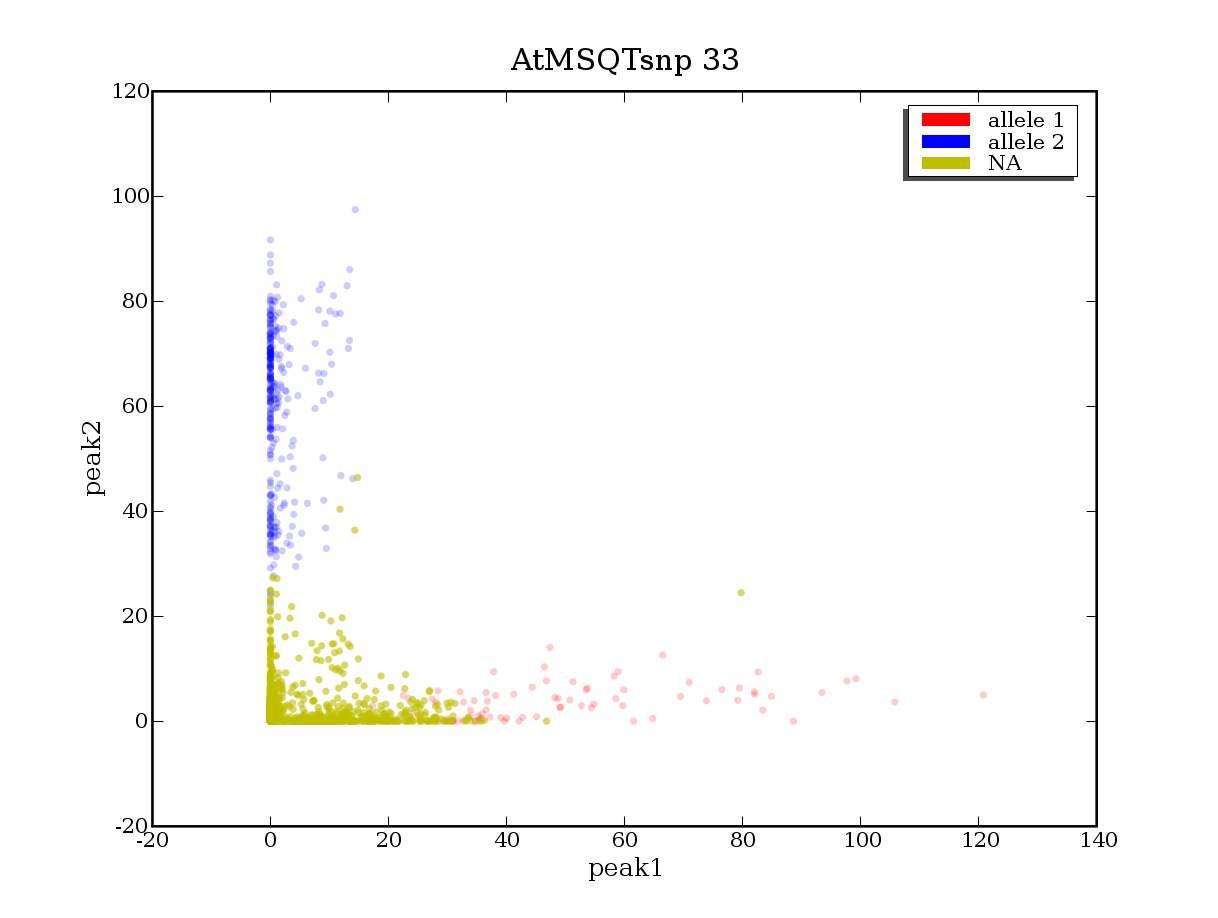
\includegraphics[width=0.5\textwidth]{figures/cluster_plot_AtMSQTsnp_33.png}
\caption{cluster plot for AtMSQTsnp 33.} \label{flAtMSQTsnp33}
\end{figure}
\begin{figure}[H]
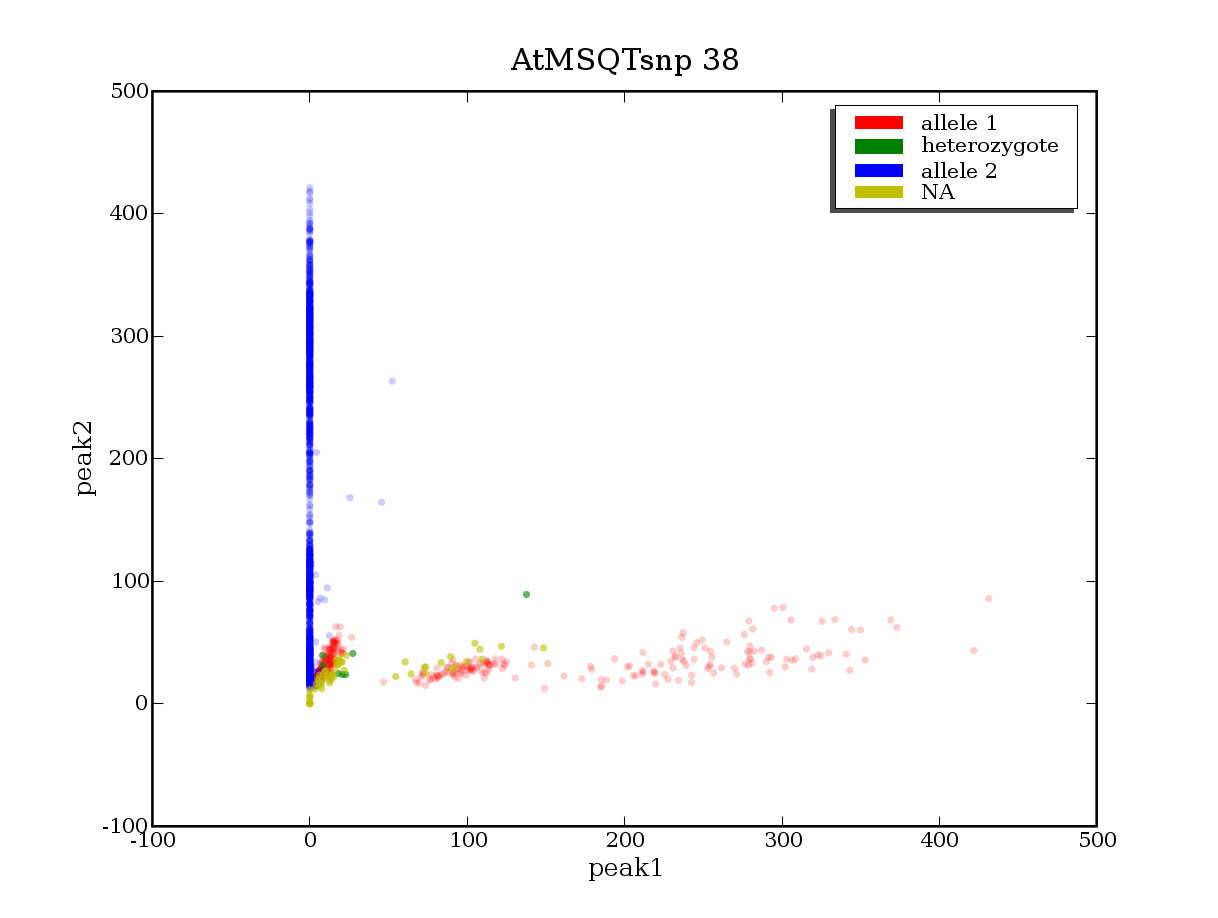
\includegraphics[width=0.5\textwidth]{figures/cluster_plot_AtMSQTsnp_38.png}
\caption{cluster plot for AtMSQTsnp 38.} \label{flAtMSQTsnp38}
\end{figure}
\begin{figure}[H]
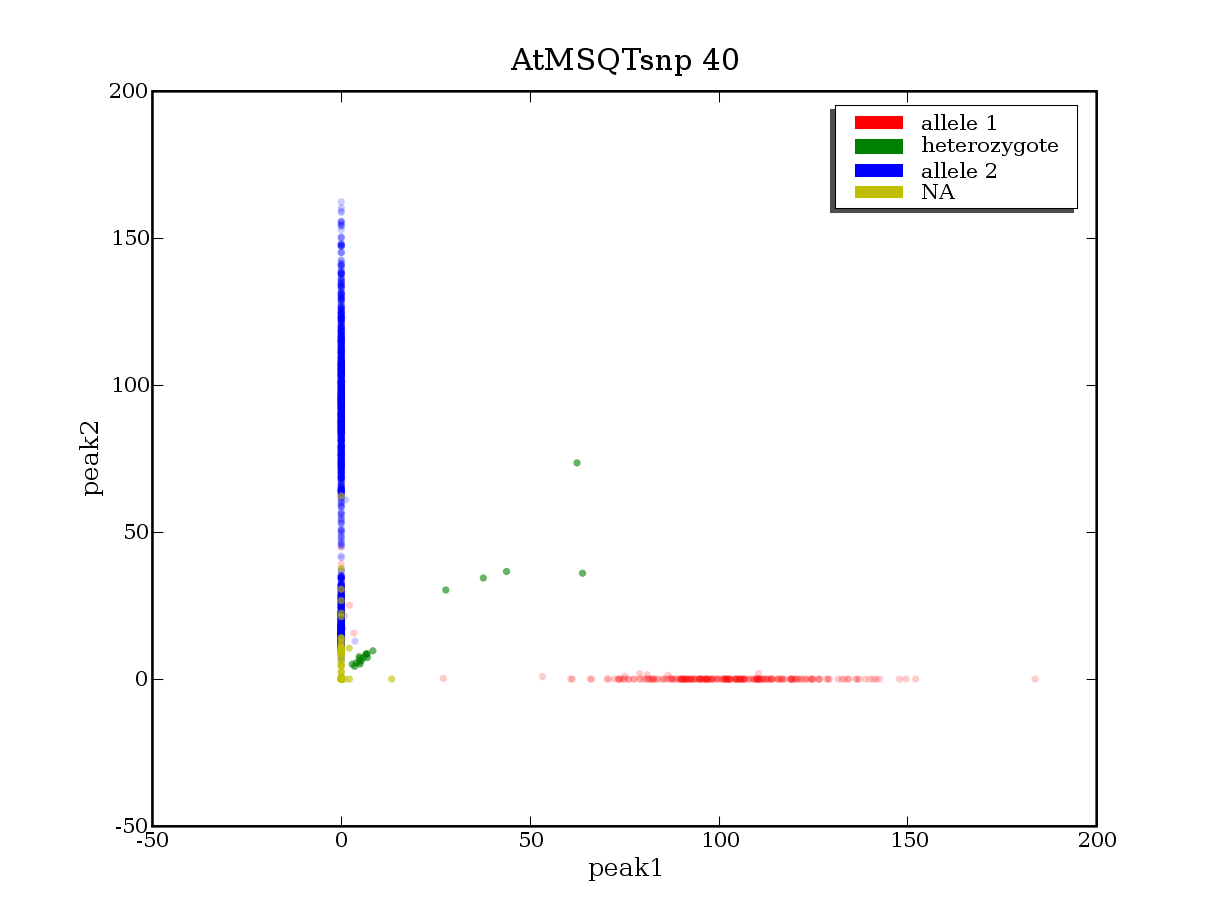
\includegraphics[width=0.5\textwidth]{figures/cluster_plot_AtMSQTsnp_40.png}
\caption{cluster plot for AtMSQTsnp 40.} \label{flAtMSQTsnp40}
\end{figure}
\begin{figure}[H]
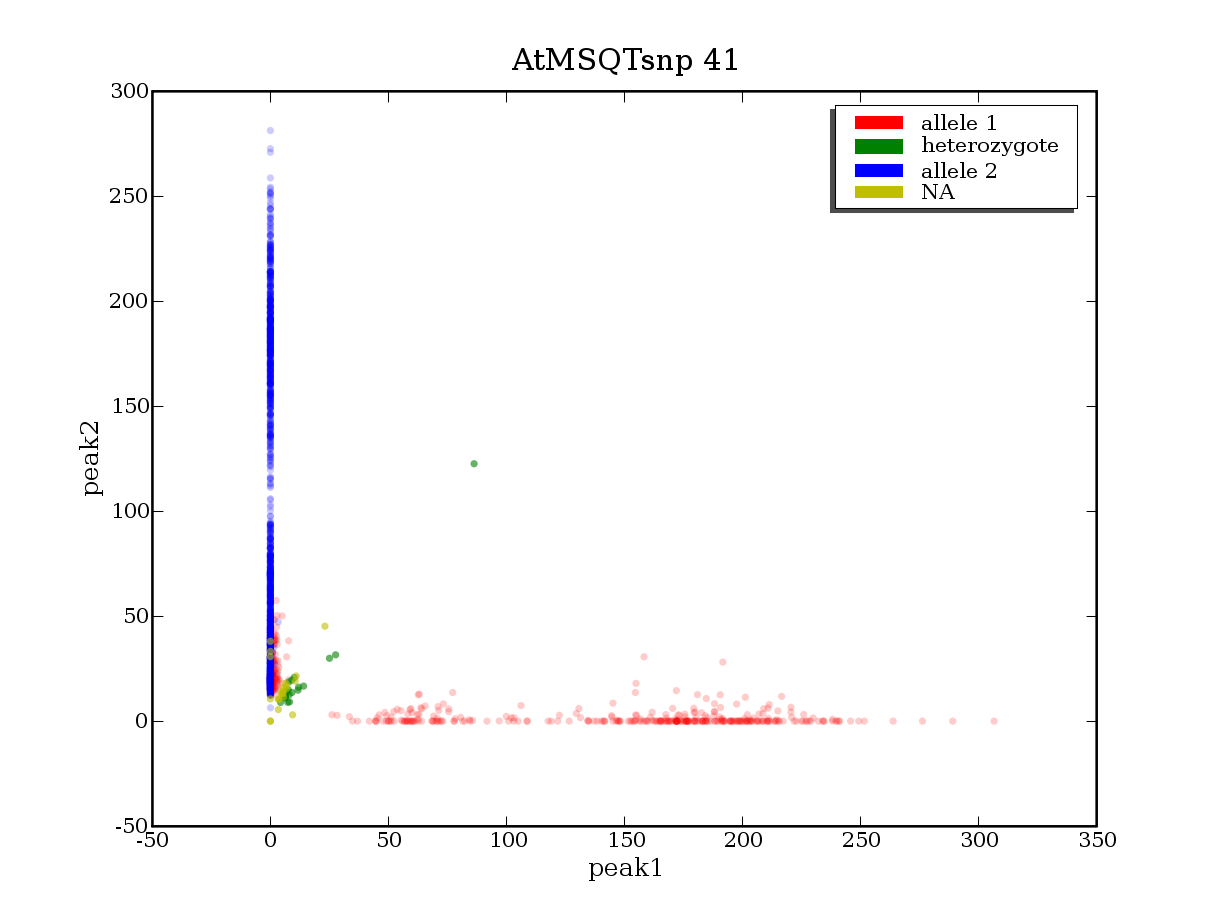
\includegraphics[width=0.5\textwidth]{figures/cluster_plot_AtMSQTsnp_41.png}
\caption{cluster plot for AtMSQTsnp 41.} \label{flAtMSQTsnp41}
\end{figure}
\begin{figure}[H]
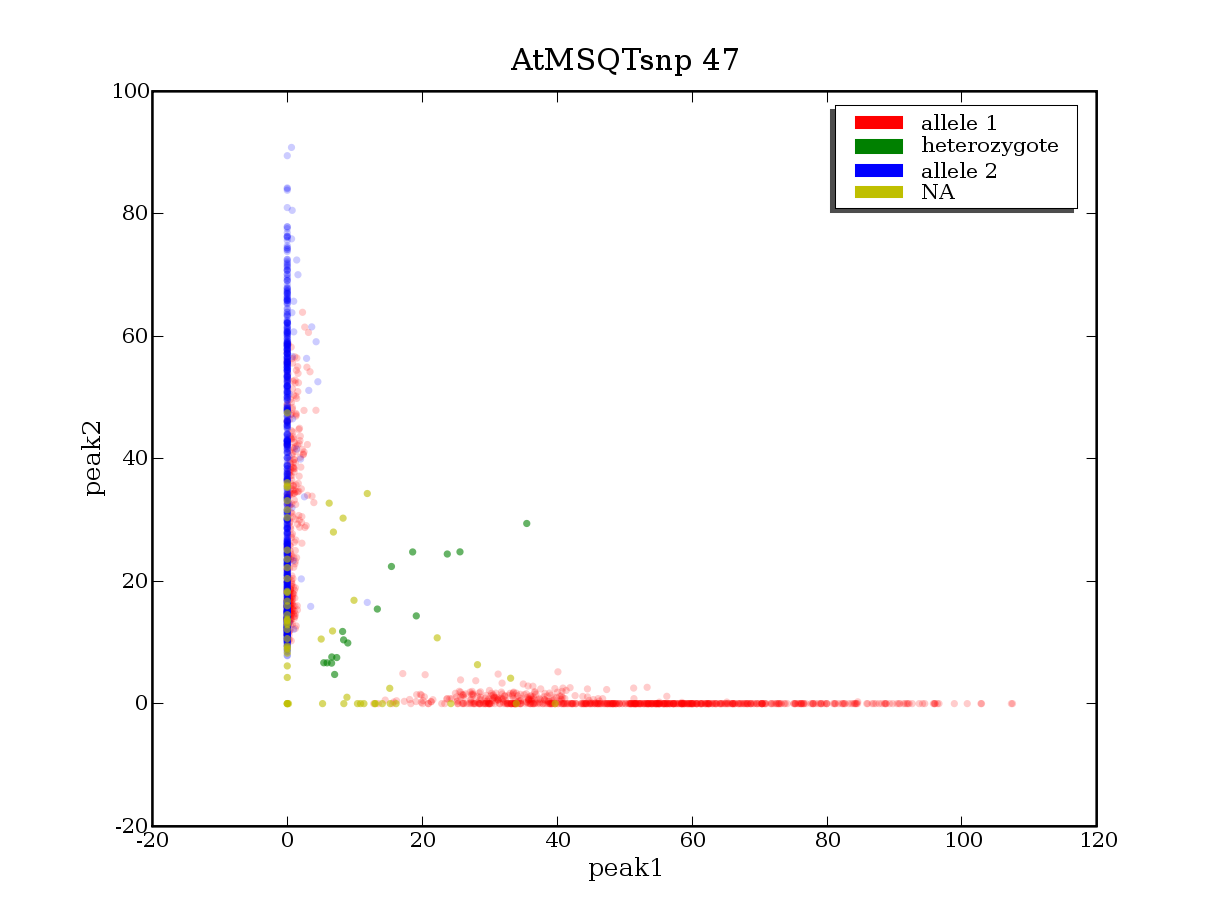
\includegraphics[width=0.5\textwidth]{figures/cluster_plot_AtMSQTsnp_47.png}
\caption{cluster plot for AtMSQTsnp 47.} \label{flAtMSQTsnp47}
\end{figure}
\begin{figure}[H]
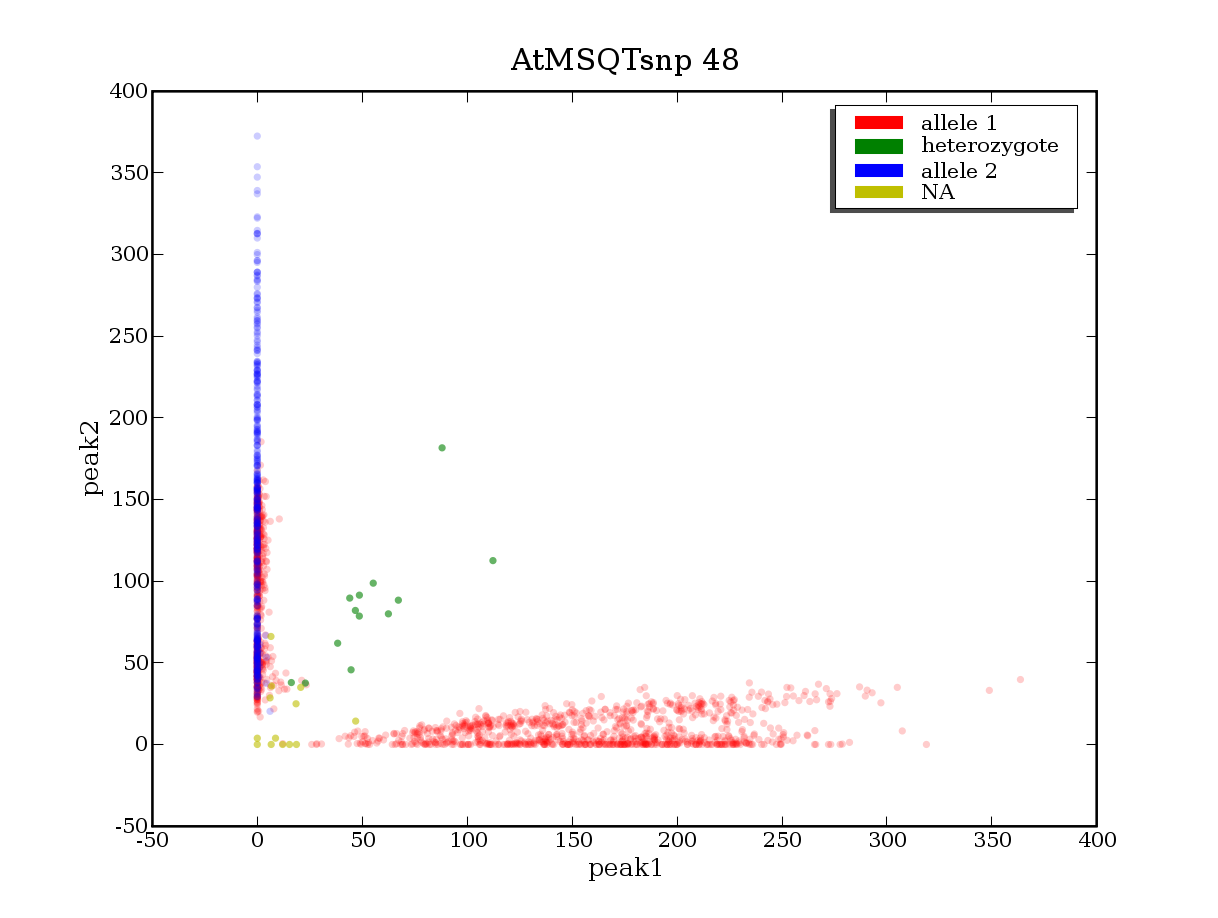
\includegraphics[width=0.5\textwidth]{figures/cluster_plot_AtMSQTsnp_48.png}
\caption{cluster plot for AtMSQTsnp 48.} \label{flAtMSQTsnp48}
\end{figure}
\begin{figure}[H]
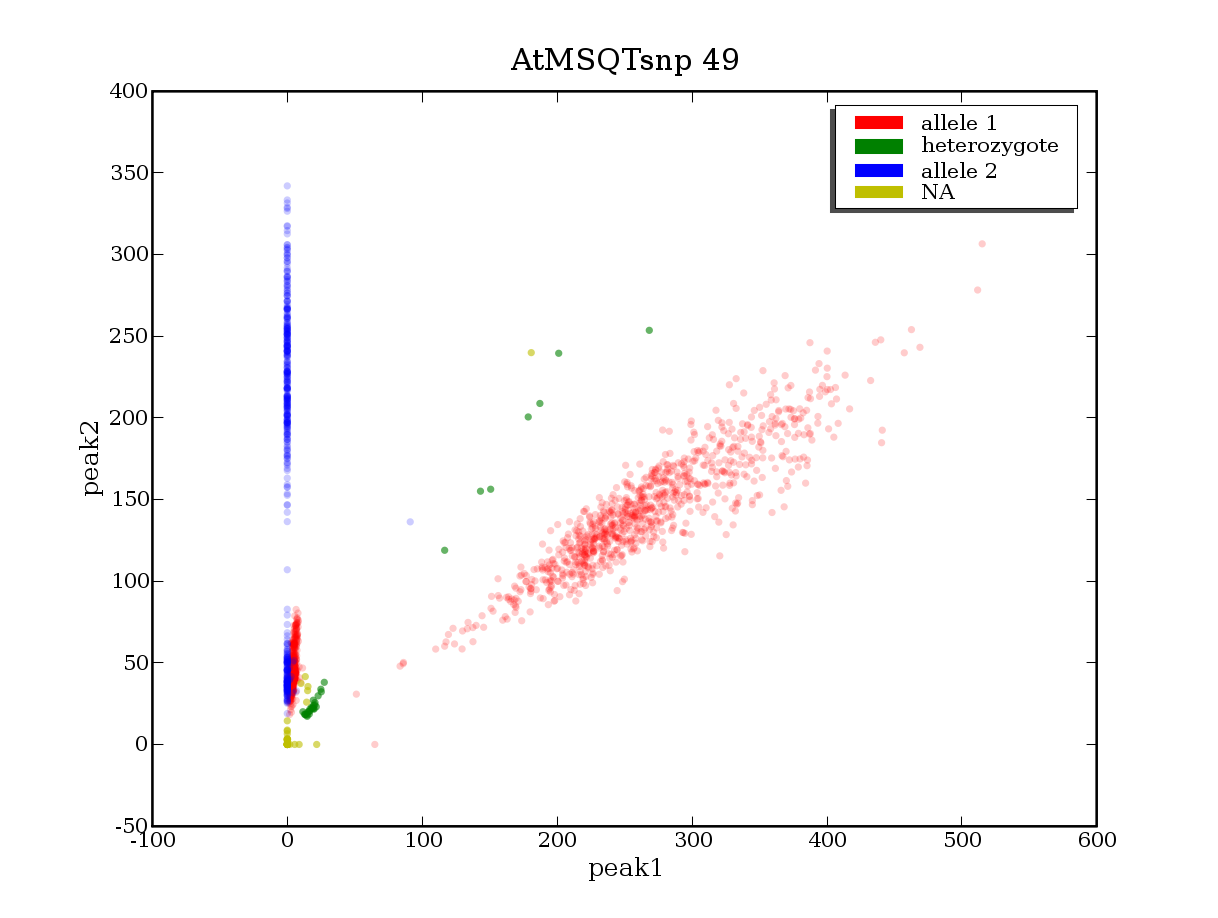
\includegraphics[width=0.5\textwidth]{figures/cluster_plot_AtMSQTsnp_49.png}
\caption{cluster plot for AtMSQTsnp 49.} \label{flAtMSQTsnp49}
\end{figure}
\begin{figure}[H]
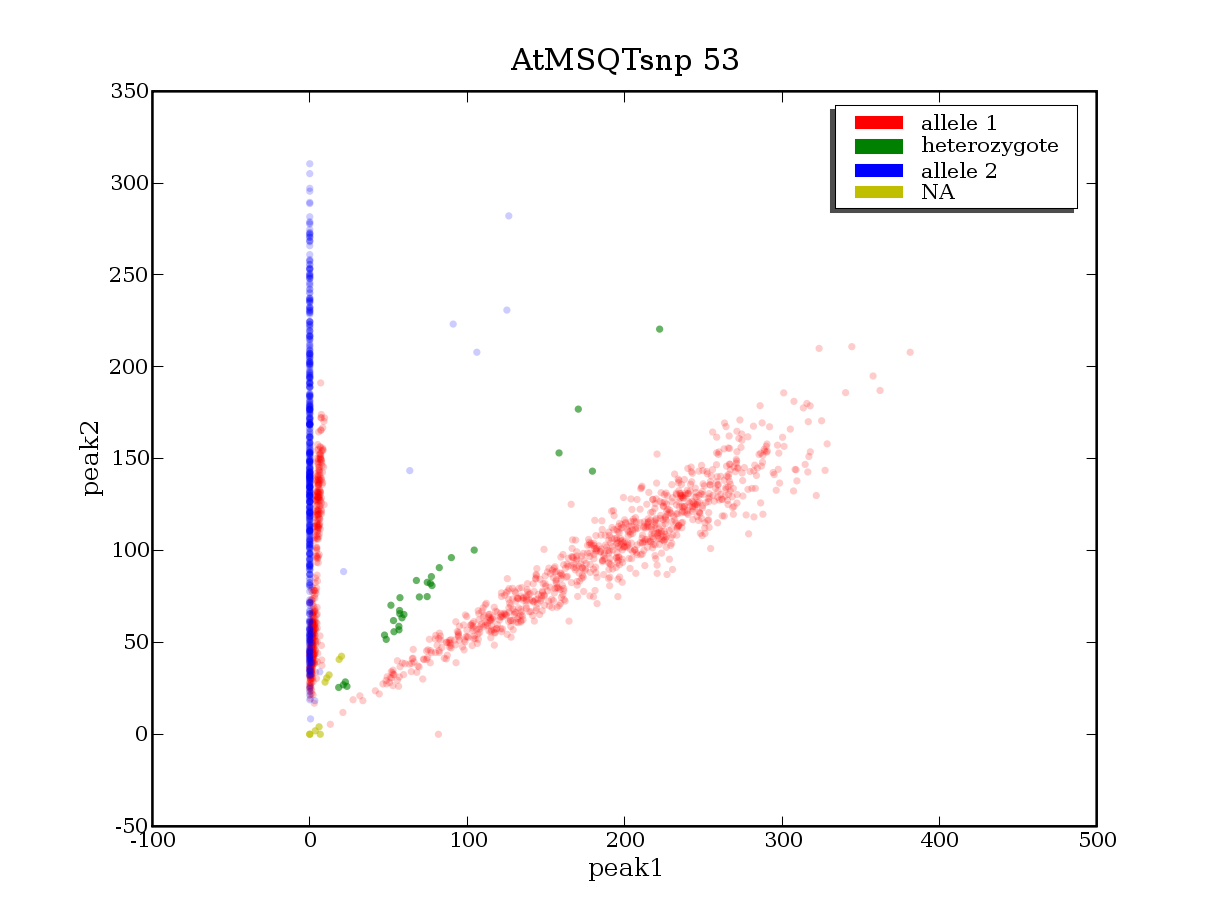
\includegraphics[width=0.5\textwidth]{figures/cluster_plot_AtMSQTsnp_53.png}
\caption{cluster plot for AtMSQTsnp 53.} \label{flAtMSQTsnp53}
\end{figure}
\begin{figure}[H]
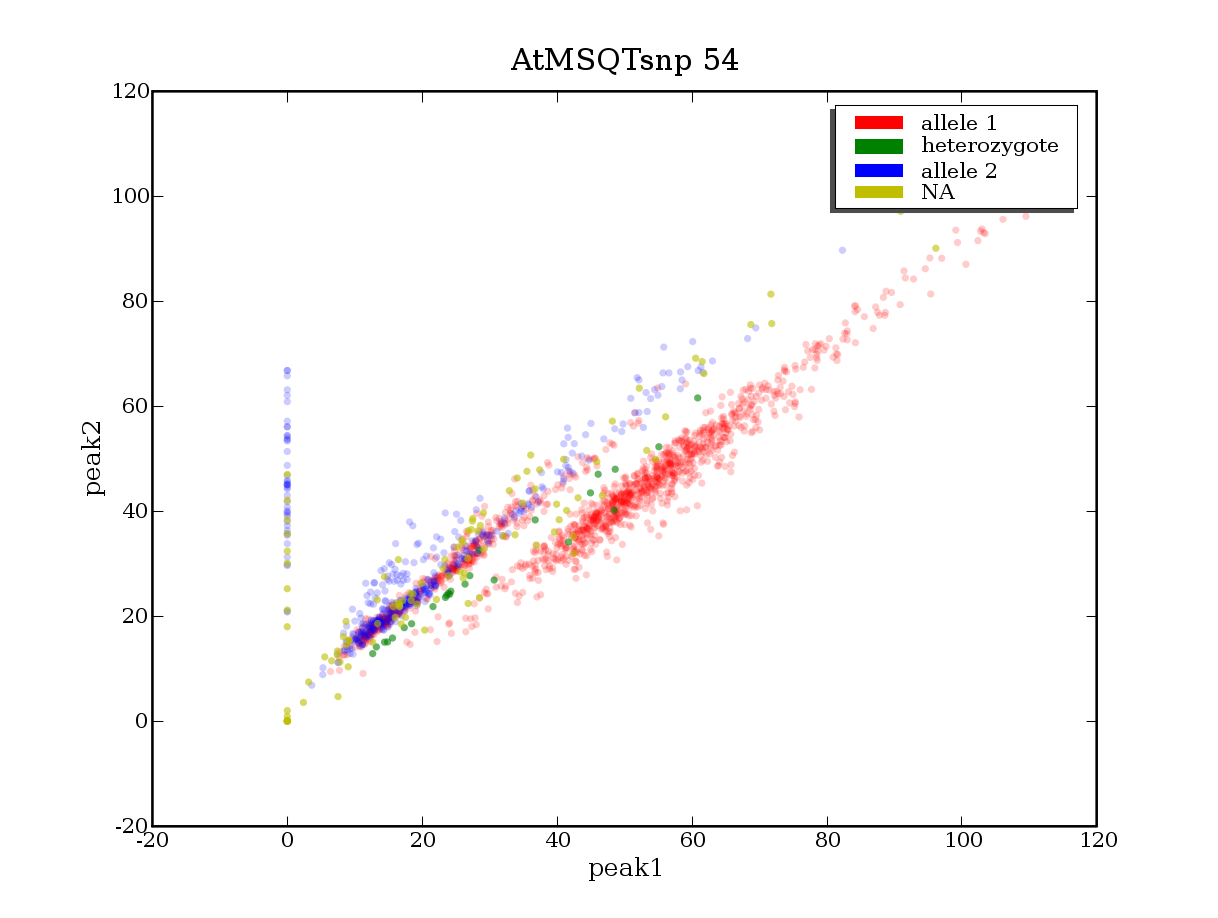
\includegraphics[width=0.5\textwidth]{figures/cluster_plot_AtMSQTsnp_54.png}
\caption{cluster plot for AtMSQTsnp 54.} \label{flAtMSQTsnp54}
\end{figure}
\begin{figure}[H]
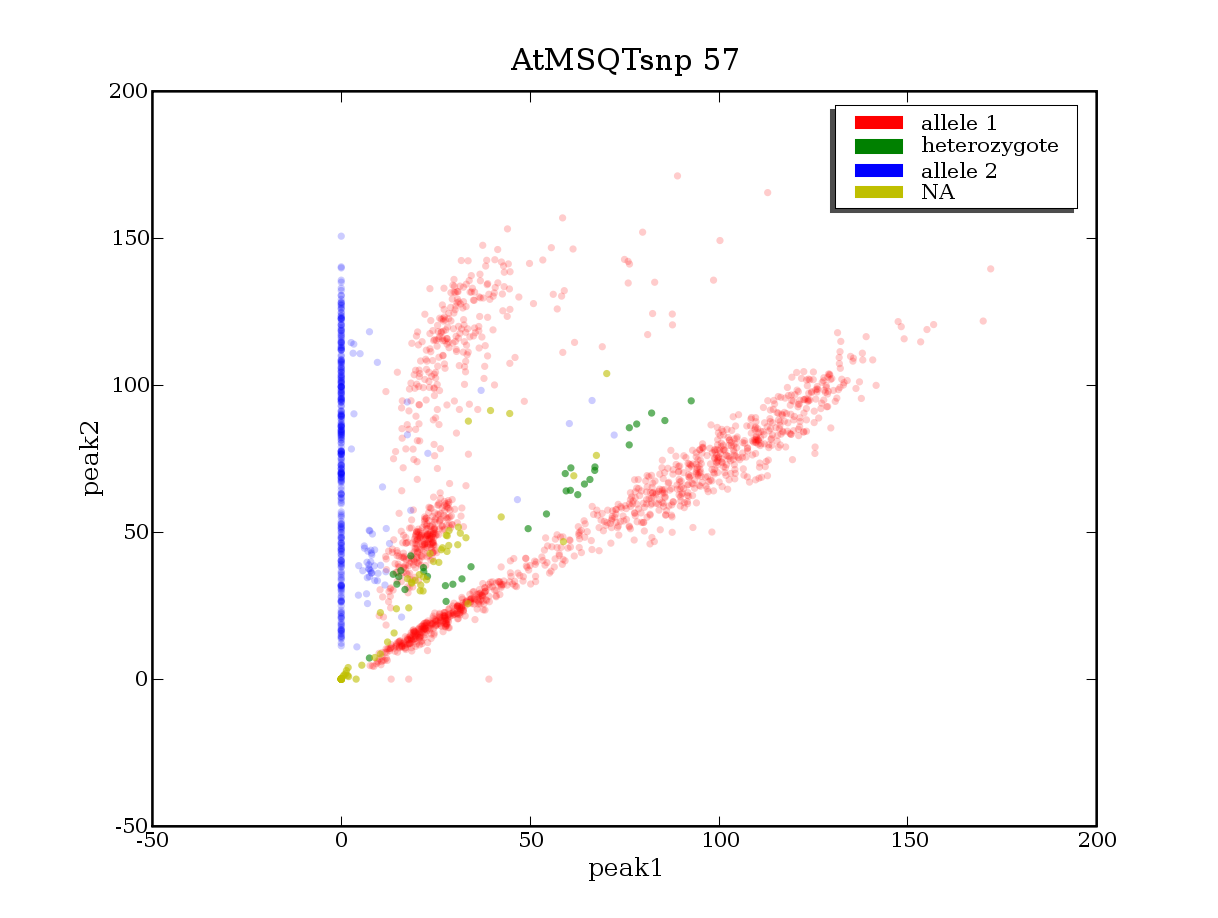
\includegraphics[width=0.5\textwidth]{figures/cluster_plot_AtMSQTsnp_57.png}
\caption{cluster plot for AtMSQTsnp 57.} \label{flAtMSQTsnp57}
\end{figure}
\begin{figure}[H]
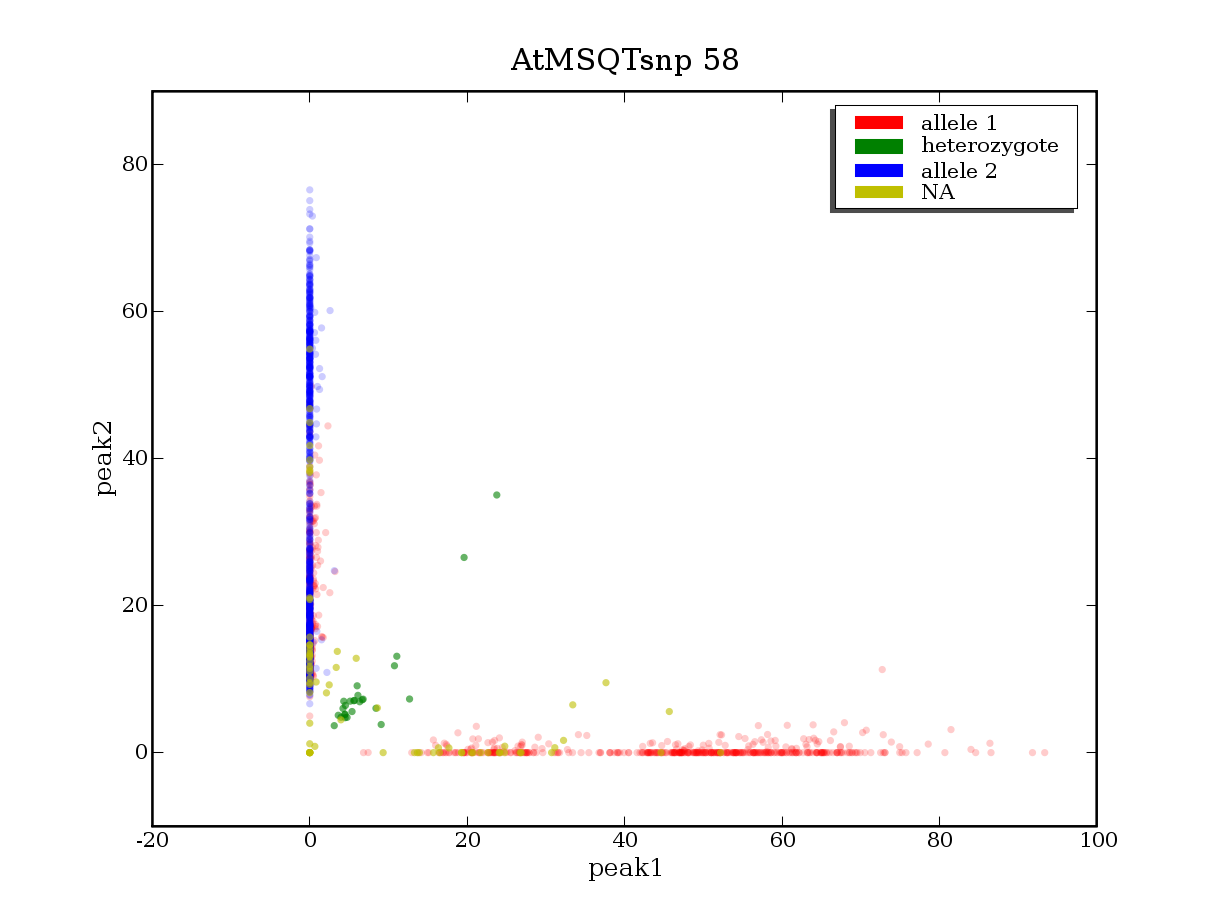
\includegraphics[width=0.5\textwidth]{figures/cluster_plot_AtMSQTsnp_58.png}
\caption{cluster plot for AtMSQTsnp 58.} \label{flAtMSQTsnp58}
\end{figure}
\begin{figure}[H]
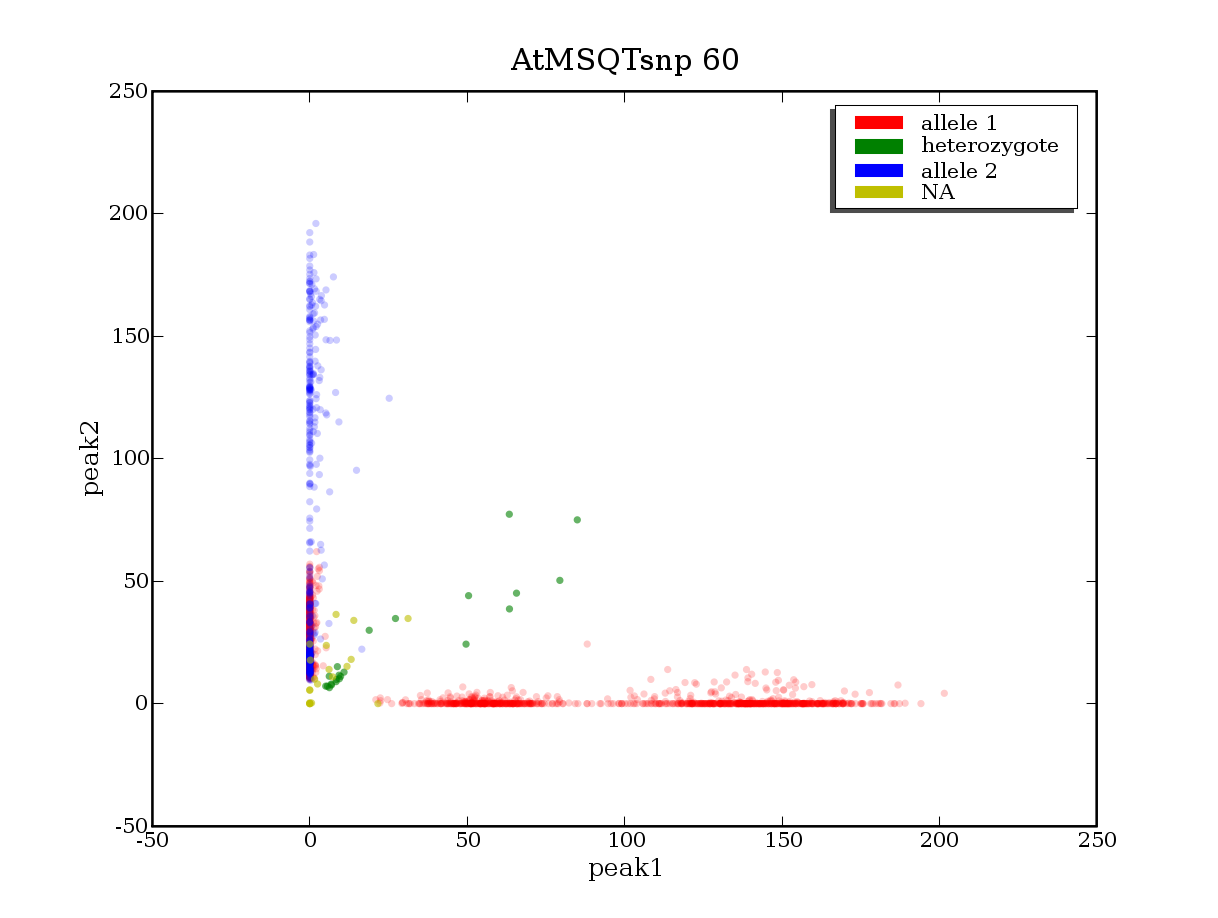
\includegraphics[width=0.5\textwidth]{figures/cluster_plot_AtMSQTsnp_60.png}
\caption{cluster plot for AtMSQTsnp 60.} \label{flAtMSQTsnp60}
\end{figure}
\begin{figure}[H]
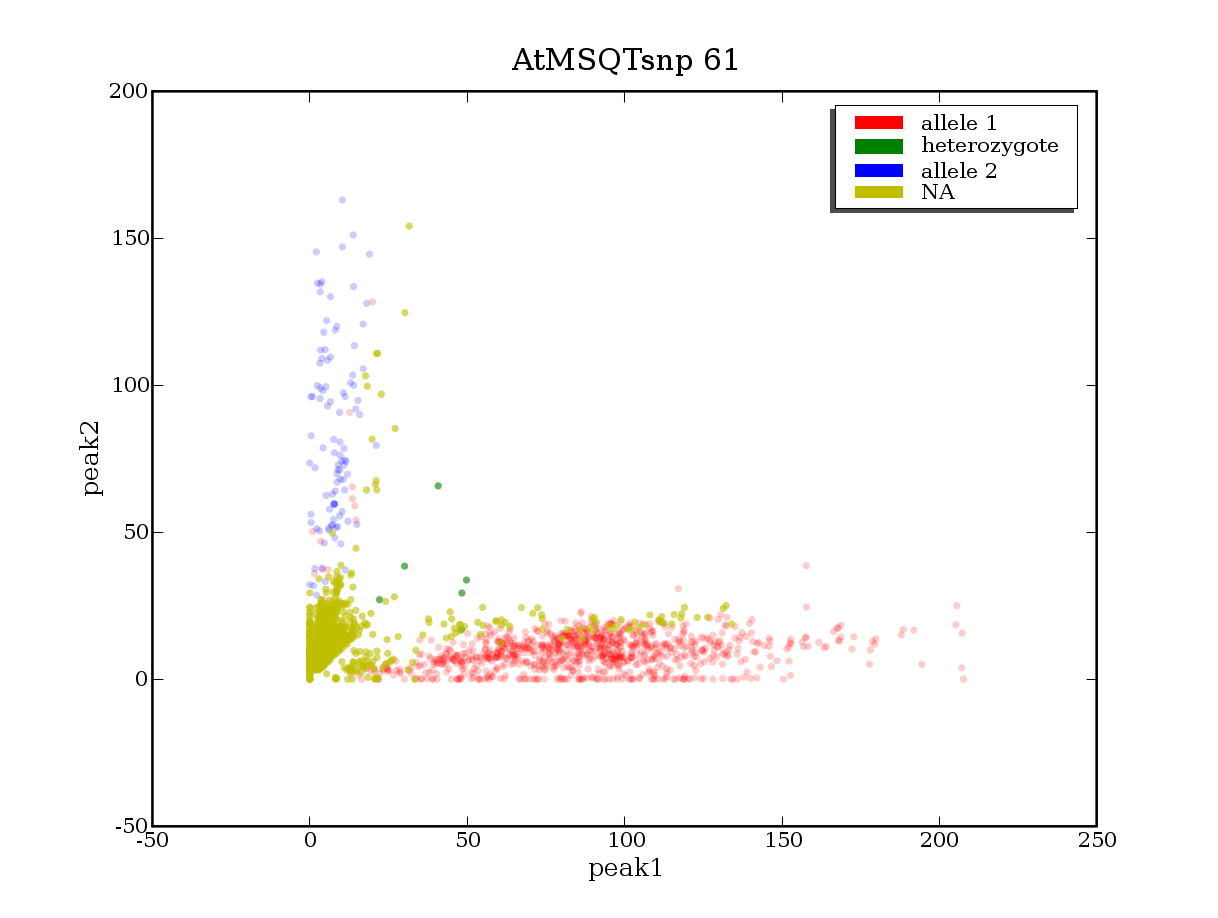
\includegraphics[width=0.5\textwidth]{figures/cluster_plot_AtMSQTsnp_61.png}
\caption{cluster plot for AtMSQTsnp 61.} \label{flAtMSQTsnp61}
\end{figure}
\begin{figure}[H]
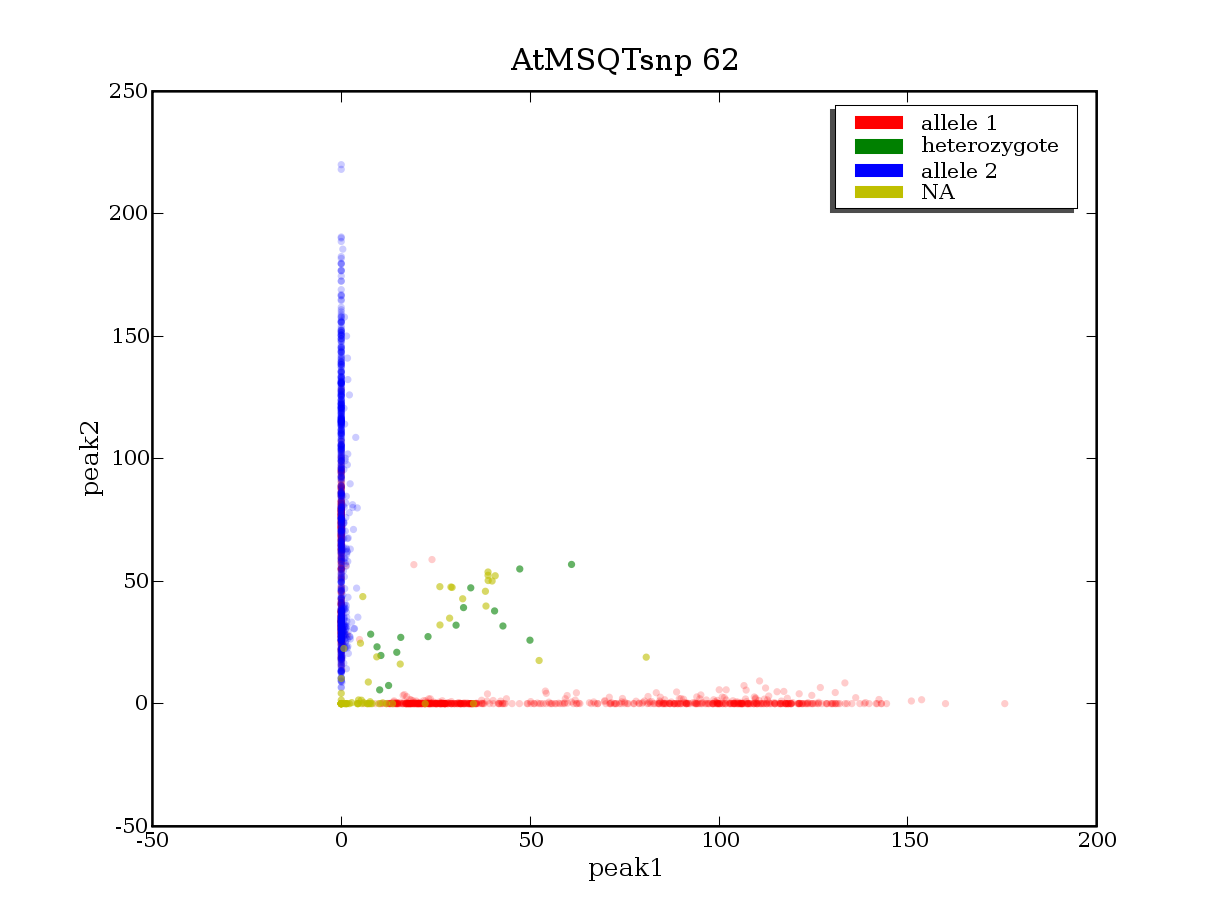
\includegraphics[width=0.5\textwidth]{figures/cluster_plot_AtMSQTsnp_62.png}
\caption{cluster plot for AtMSQTsnp 62.} \label{flAtMSQTsnp62}
\end{figure}
\begin{figure}[H]
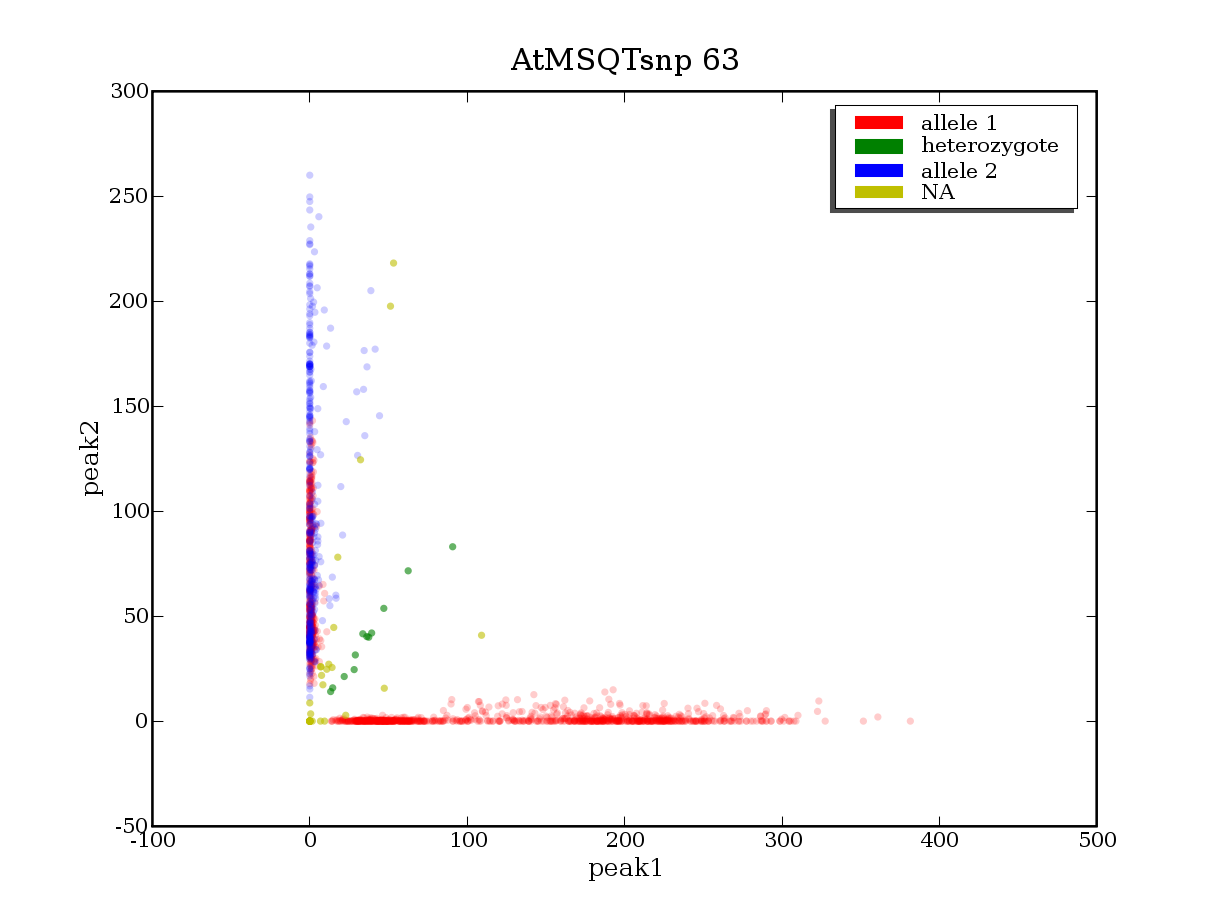
\includegraphics[width=0.5\textwidth]{figures/cluster_plot_AtMSQTsnp_63.png}
\caption{cluster plot for AtMSQTsnp 63.} \label{flAtMSQTsnp63}
\end{figure}
\begin{figure}[H]
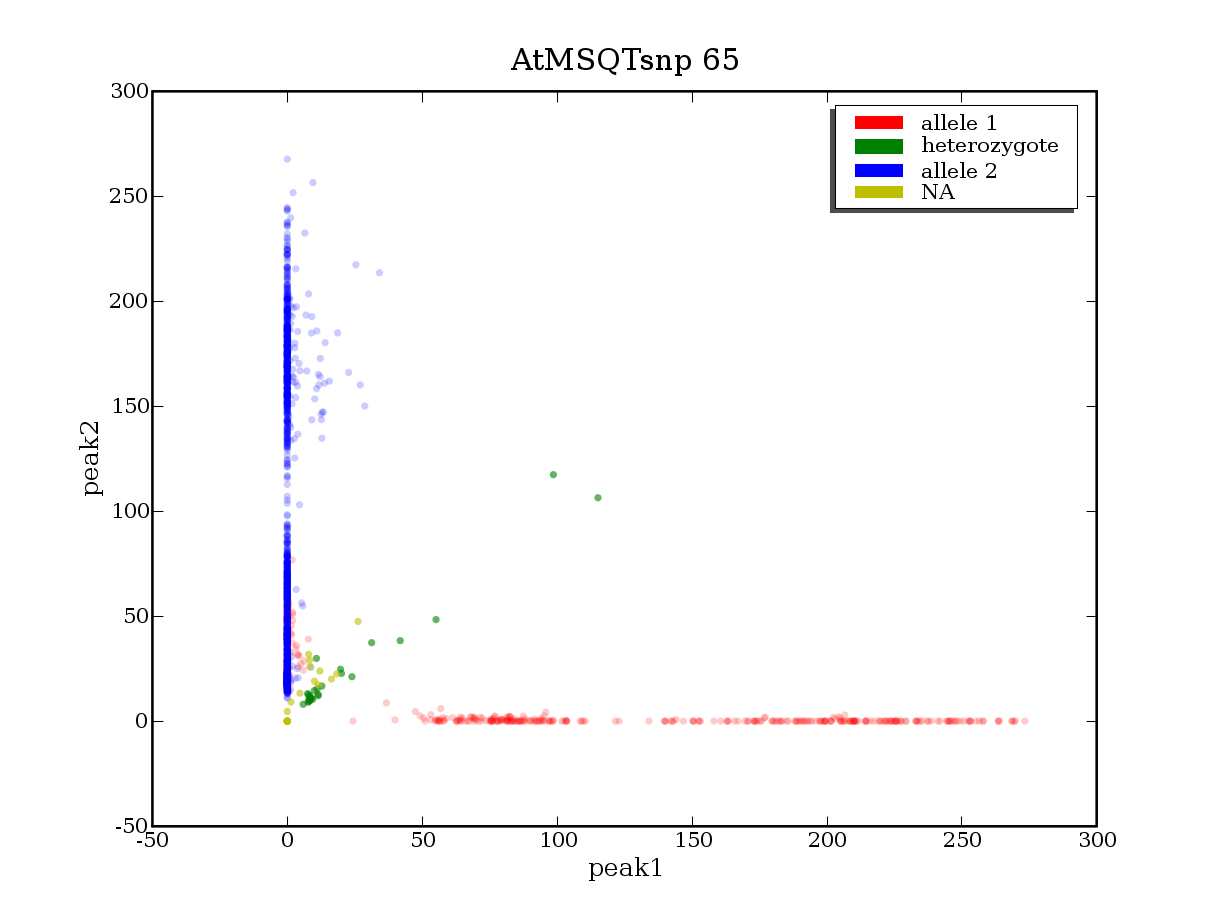
\includegraphics[width=0.5\textwidth]{figures/cluster_plot_AtMSQTsnp_65.png}
\caption{cluster plot for AtMSQTsnp 65.} \label{flAtMSQTsnp65}
\end{figure}
\begin{figure}[H]
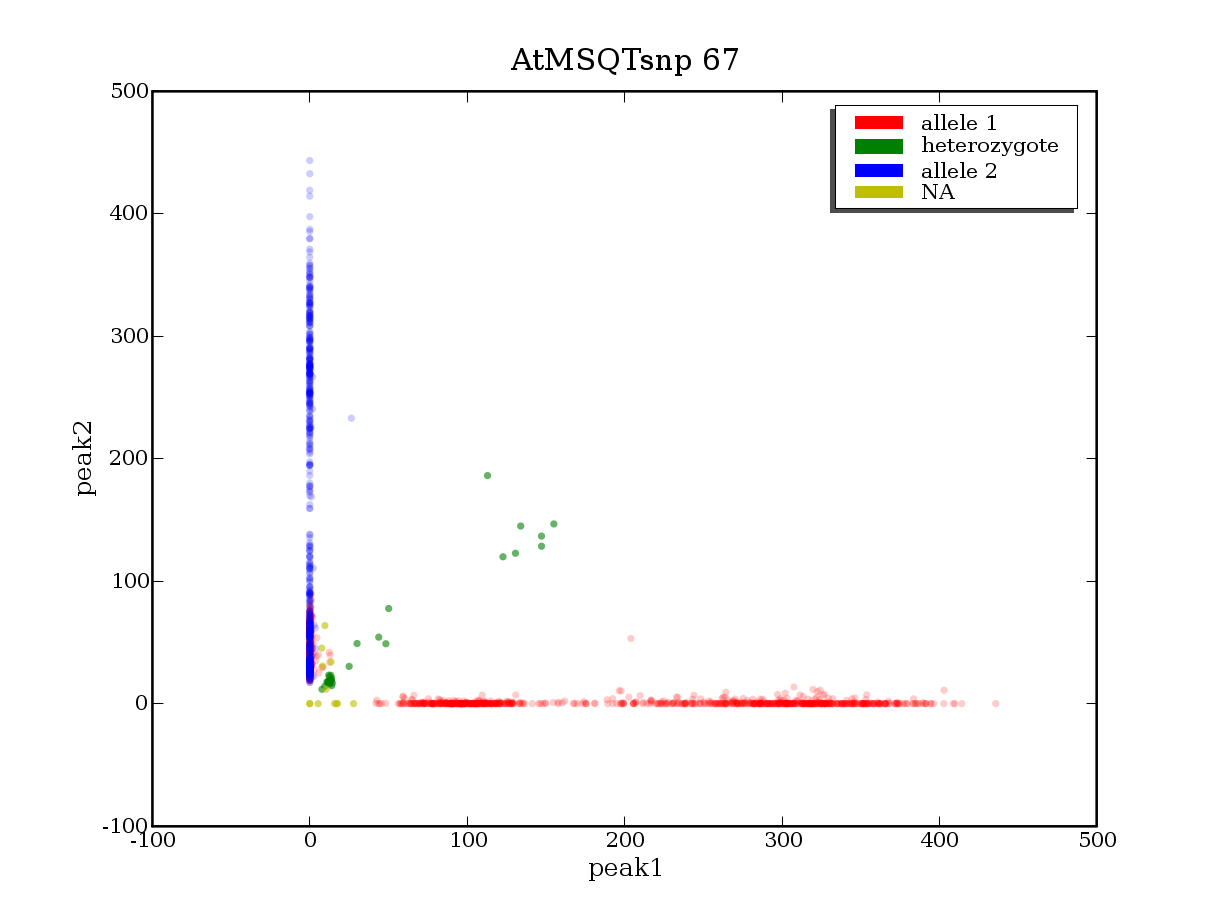
\includegraphics[width=0.5\textwidth]{figures/cluster_plot_AtMSQTsnp_67.png}
\caption{cluster plot for AtMSQTsnp 67.} \label{flAtMSQTsnp67}
\end{figure}
\begin{figure}[H]
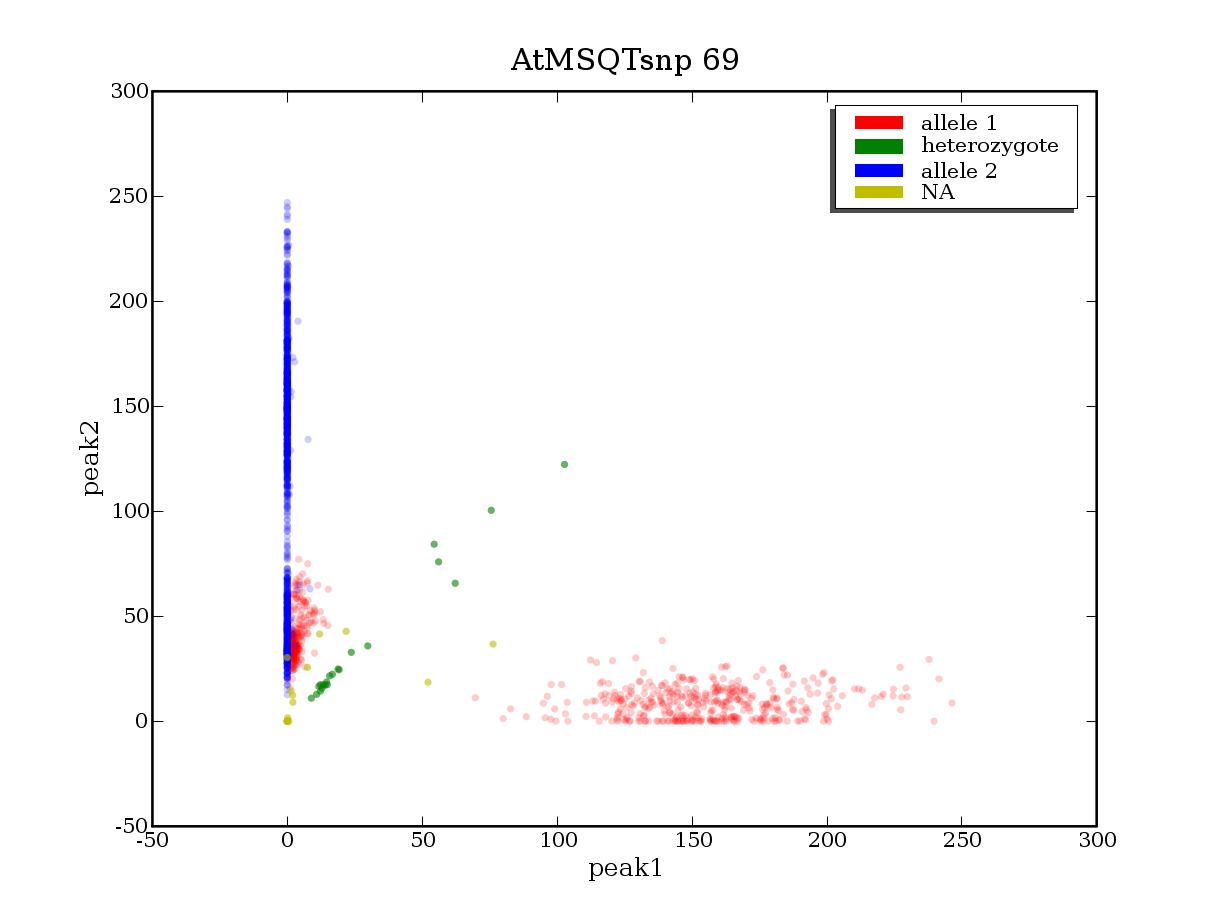
\includegraphics[width=0.5\textwidth]{figures/cluster_plot_AtMSQTsnp_69.png}
\caption{cluster plot for AtMSQTsnp 69.} \label{flAtMSQTsnp69}
\end{figure}
\begin{figure}[H]
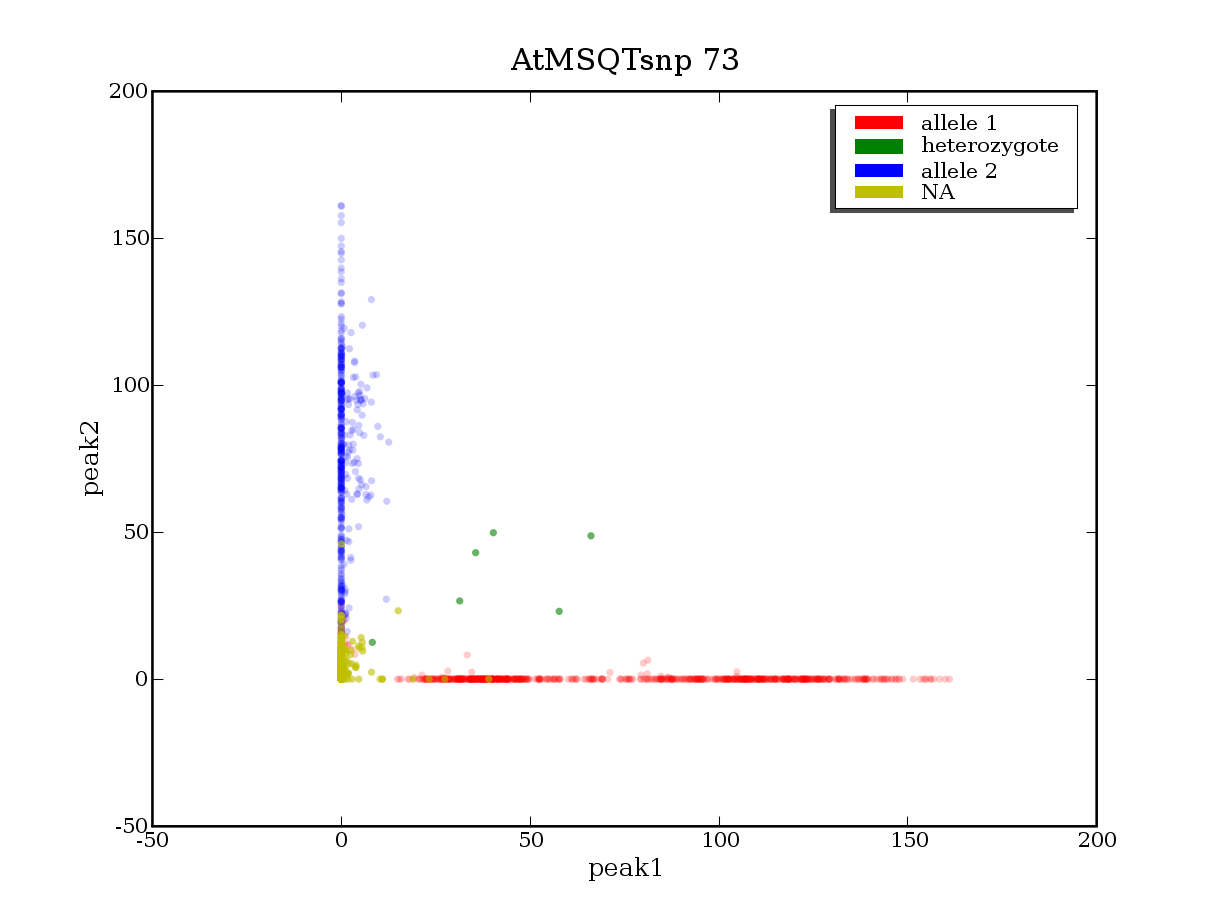
\includegraphics[width=0.5\textwidth]{figures/cluster_plot_AtMSQTsnp_73.png}
\caption{cluster plot for AtMSQTsnp 73.} \label{flAtMSQTsnp73}
\end{figure}
\begin{figure}[H]
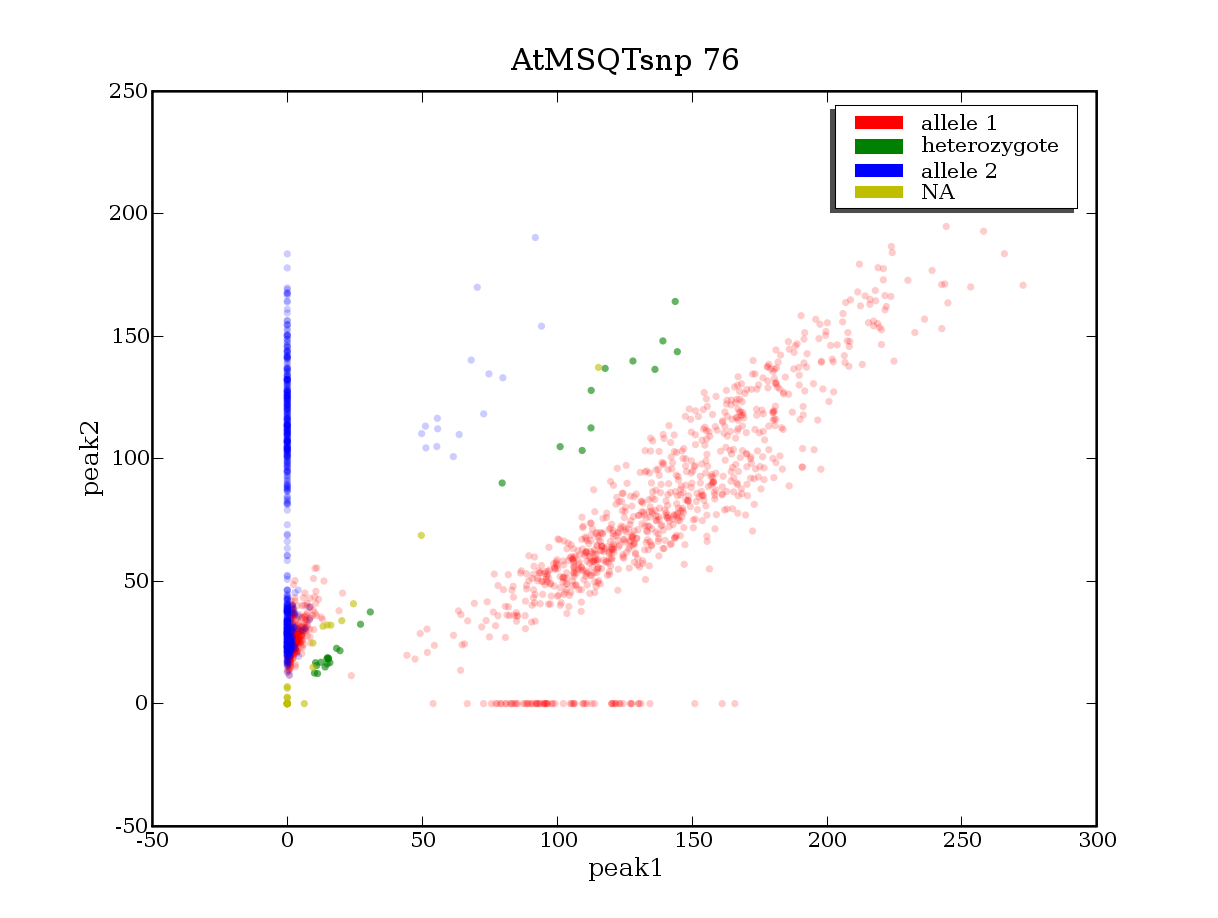
\includegraphics[width=0.5\textwidth]{figures/cluster_plot_AtMSQTsnp_76.png}
\caption{cluster plot for AtMSQTsnp 76.} \label{flAtMSQTsnp76}
\end{figure}
\begin{figure}[H]
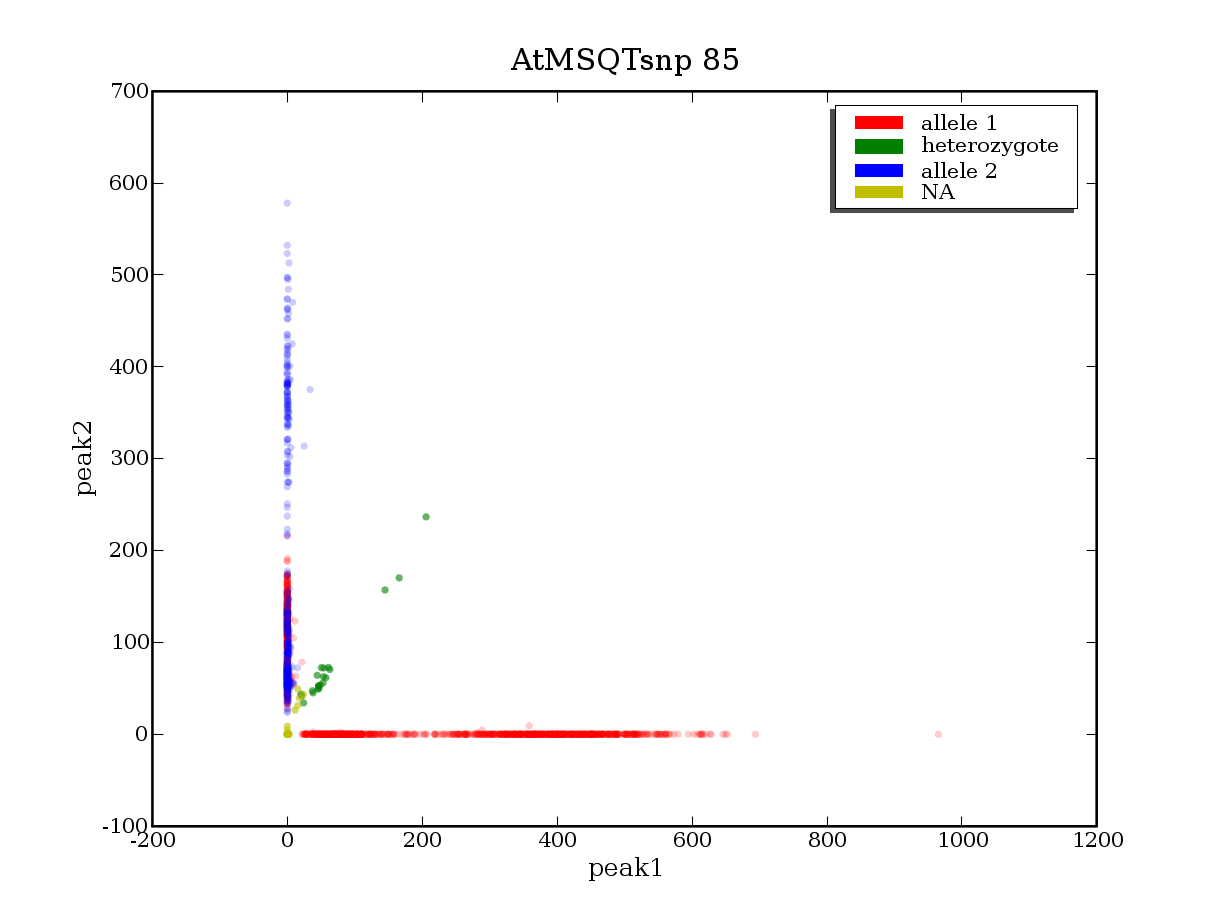
\includegraphics[width=0.5\textwidth]{figures/cluster_plot_AtMSQTsnp_85.png}
\caption{cluster plot for AtMSQTsnp 85.} \label{flAtMSQTsnp85}
\end{figure}
\begin{figure}[H]
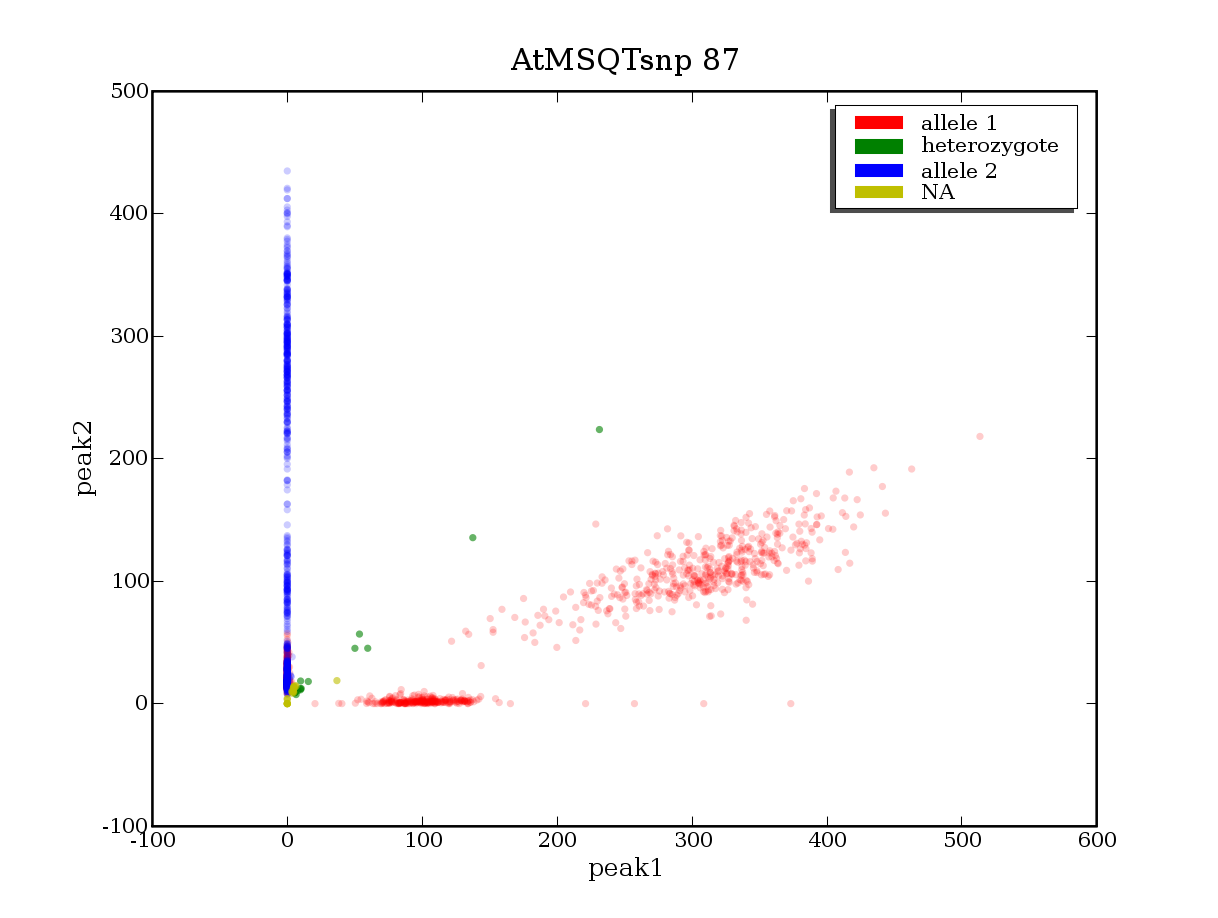
\includegraphics[width=0.5\textwidth]{figures/cluster_plot_AtMSQTsnp_87.png}
\caption{cluster plot for AtMSQTsnp 87.} \label{flAtMSQTsnp87}
\end{figure}
\begin{figure}[H]
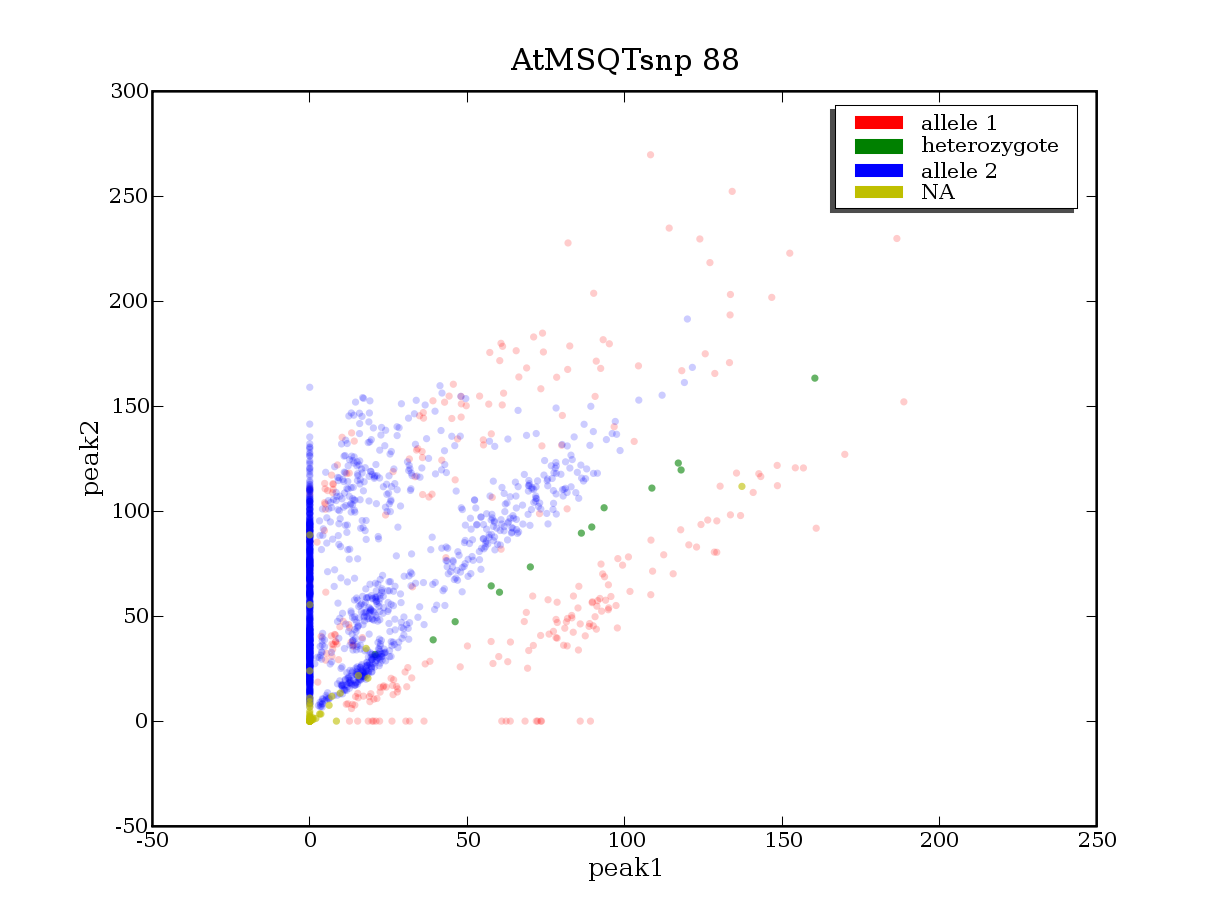
\includegraphics[width=0.5\textwidth]{figures/cluster_plot_AtMSQTsnp_88.png}
\caption{cluster plot for AtMSQTsnp 88.} \label{flAtMSQTsnp88}
\end{figure}
\begin{figure}[H]
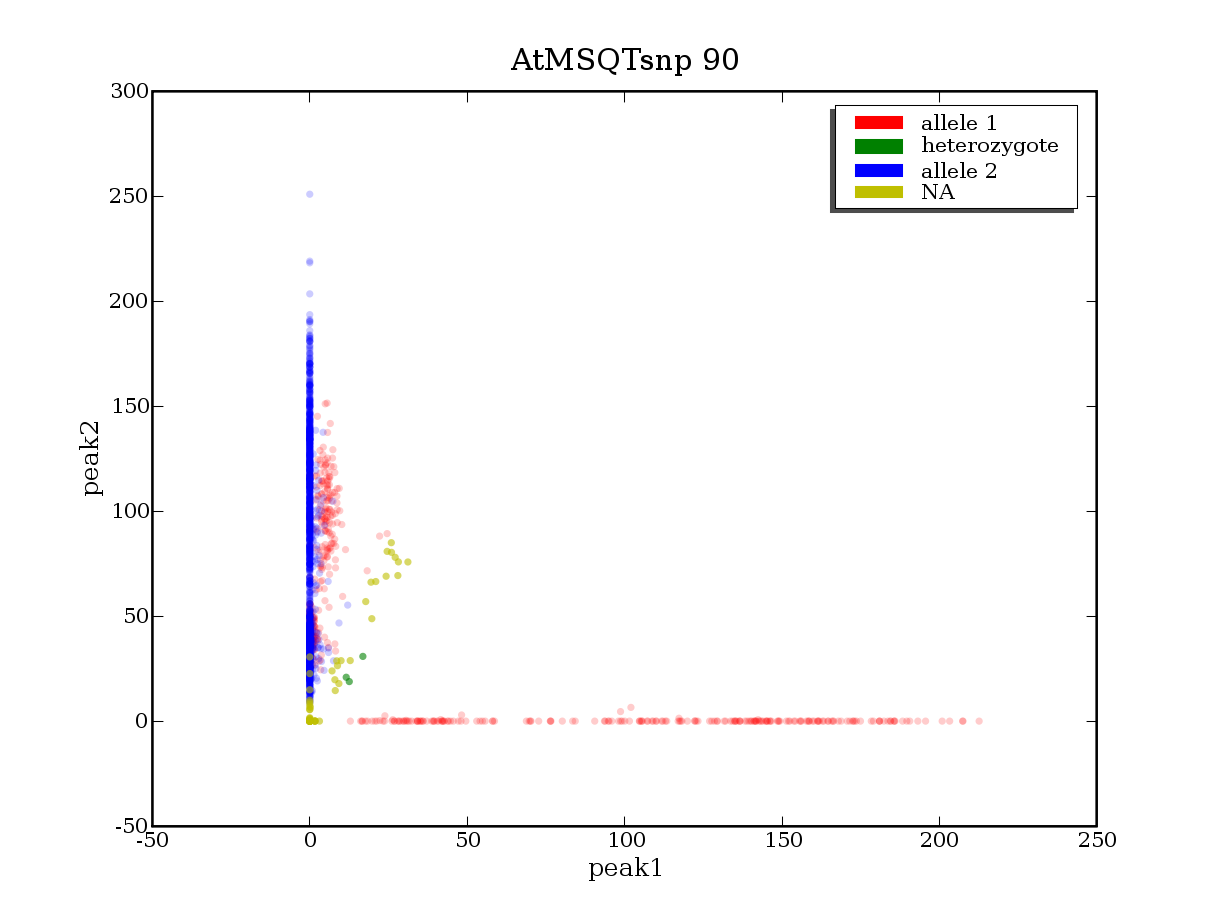
\includegraphics[width=0.5\textwidth]{figures/cluster_plot_AtMSQTsnp_90.png}
\caption{cluster plot for AtMSQTsnp 90.} \label{flAtMSQTsnp90}
\end{figure}
\begin{figure}[H]
\includegraphics[width=0.5\textwidth]{figures/cluster_plot_AtMSQTsnp_91.png}
\caption{cluster plot for AtMSQTsnp 91.} \label{flAtMSQTsnp91}
\end{figure}
\begin{figure}[H]
\includegraphics[width=0.5\textwidth]{figures/cluster_plot_AtMSQTsnp_92.png}
\caption{cluster plot for AtMSQTsnp 92.} \label{flAtMSQTsnp92}
\end{figure}
\begin{figure}[H]
\includegraphics[width=0.5\textwidth]{figures/cluster_plot_AtMSQTsnp_97.png}
\caption{cluster plot for AtMSQTsnp 97.} \label{flAtMSQTsnp97}
\end{figure}
\begin{figure}[H]
\includegraphics[width=0.5\textwidth]{figures/cluster_plot_AtMSQTsnp_100.png}
\caption{cluster plot for AtMSQTsnp 100.} \label{flAtMSQTsnp100}
\end{figure}
\begin{figure}[H]
\includegraphics[width=0.5\textwidth]{figures/cluster_plot_AtMSQTsnp_101.png}
\caption{cluster plot for AtMSQTsnp 101.} \label{flAtMSQTsnp101}
\end{figure}
\begin{figure}[H]
\includegraphics[width=0.5\textwidth]{figures/cluster_plot_AtMSQTsnp_104.png}
\caption{cluster plot for AtMSQTsnp 104.} \label{flAtMSQTsnp104}
\end{figure}
\begin{figure}[H]
\includegraphics[width=0.5\textwidth]{figures/cluster_plot_AtMSQTsnp_108.png}
\caption{cluster plot for AtMSQTsnp 108.} \label{flAtMSQTsnp108}
\end{figure}
\begin{figure}[H]
\includegraphics[width=0.5\textwidth]{figures/cluster_plot_AtMSQTsnp_114.png}
\caption{cluster plot for AtMSQTsnp 114.} \label{flAtMSQTsnp114}
\end{figure}
\begin{figure}[H]
\includegraphics[width=0.5\textwidth]{figures/cluster_plot_AtMSQTsnp_118.png}
\caption{cluster plot for AtMSQTsnp 118.} \label{flAtMSQTsnp118}
\end{figure}
\begin{figure}[H]
\includegraphics[width=0.5\textwidth]{figures/cluster_plot_AtMSQTsnp_123.png}
\caption{cluster plot for AtMSQTsnp 123.} \label{flAtMSQTsnp123}
\end{figure}
\begin{figure}[H]
\includegraphics[width=0.5\textwidth]{figures/cluster_plot_AtMSQTsnp_126.png}
\caption{cluster plot for AtMSQTsnp 126.} \label{flAtMSQTsnp126}
\end{figure}
\begin{figure}[H]
\includegraphics[width=0.5\textwidth]{figures/cluster_plot_AtMSQTsnp_128.png}
\caption{cluster plot for AtMSQTsnp 128.} \label{flAtMSQTsnp128}
\end{figure}
\begin{figure}[H]
\includegraphics[width=0.5\textwidth]{figures/cluster_plot_AtMSQTsnp_129.png}
\caption{cluster plot for AtMSQTsnp 129.} \label{flAtMSQTsnp129}
\end{figure}
\begin{figure}[H]
\includegraphics[width=0.5\textwidth]{figures/cluster_plot_AtMSQTsnp_130.png}
\caption{cluster plot for AtMSQTsnp 130.} \label{flAtMSQTsnp130}
\end{figure}
\begin{figure}[H]
\includegraphics[width=0.5\textwidth]{figures/cluster_plot_AtMSQTsnp_132.png}
\caption{cluster plot for AtMSQTsnp 132.} \label{flAtMSQTsnp132}
\end{figure}
\begin{figure}[H]
\includegraphics[width=0.5\textwidth]{figures/cluster_plot_AtMSQTsnp_138.png}
\caption{cluster plot for AtMSQTsnp 138.} \label{flAtMSQTsnp138}
\end{figure}
\begin{figure}[H]
\includegraphics[width=0.5\textwidth]{figures/cluster_plot_AtMSQTsnp_140.png}
\caption{cluster plot for AtMSQTsnp 140.} \label{flAtMSQTsnp140}
\end{figure}
\begin{figure}[H]
\includegraphics[width=0.5\textwidth]{figures/cluster_plot_AtMSQTsnp_142.png}
\caption{cluster plot for AtMSQTsnp 142.} \label{flAtMSQTsnp142}
\end{figure}
\begin{figure}[H]
\includegraphics[width=0.5\textwidth]{figures/cluster_plot_AtMSQTsnp_143.png}
\caption{cluster plot for AtMSQTsnp 143.} \label{flAtMSQTsnp143}
\end{figure}
\begin{figure}[H]
\includegraphics[width=0.5\textwidth]{figures/cluster_plot_AtMSQTsnp_145.png}
\caption{cluster plot for AtMSQTsnp 145.} \label{flAtMSQTsnp145}
\end{figure}
\begin{figure}[H]
\includegraphics[width=0.5\textwidth]{figures/cluster_plot_AtMSQTsnp_146.png}
\caption{cluster plot for AtMSQTsnp 146.} \label{flAtMSQTsnp146}
\end{figure}
\begin{figure}[H]
\includegraphics[width=0.5\textwidth]{figures/cluster_plot_AtMSQTsnp_155.png}
\caption{cluster plot for AtMSQTsnp 155.} \label{flAtMSQTsnp155}
\end{figure}
\begin{figure}[H]
\includegraphics[width=0.5\textwidth]{figures/cluster_plot_AtMSQTsnp_156.png}
\caption{cluster plot for AtMSQTsnp 156.} \label{flAtMSQTsnp156}
\end{figure}
\begin{figure}[H]
\includegraphics[width=0.5\textwidth]{figures/cluster_plot_AtMSQTsnp_159.png}
\caption{cluster plot for AtMSQTsnp 159.} \label{flAtMSQTsnp159}
\end{figure}
\begin{figure}[H]
\includegraphics[width=0.5\textwidth]{figures/cluster_plot_AtMSQTsnp_164.png}
\caption{cluster plot for AtMSQTsnp 164.} \label{flAtMSQTsnp164}
\end{figure}
\begin{figure}[H]
\includegraphics[width=0.5\textwidth]{figures/cluster_plot_AtMSQTsnp_169.png}
\caption{cluster plot for AtMSQTsnp 169.} \label{flAtMSQTsnp169}
\end{figure}
\begin{figure}[H]
\includegraphics[width=0.5\textwidth]{figures/cluster_plot_AtMSQTsnp_170.png}
\caption{cluster plot for AtMSQTsnp 170.} \label{flAtMSQTsnp170}
\end{figure}
\begin{figure}[H]
\includegraphics[width=0.5\textwidth]{figures/cluster_plot_AtMSQTsnp_173.png}
\caption{cluster plot for AtMSQTsnp 173.} \label{flAtMSQTsnp173}
\end{figure}
\begin{figure}[H]
\includegraphics[width=0.5\textwidth]{figures/cluster_plot_AtMSQTsnp_174.png}
\caption{cluster plot for AtMSQTsnp 174.} \label{flAtMSQTsnp174}
\end{figure}
\begin{figure}[H]
\includegraphics[width=0.5\textwidth]{figures/cluster_plot_AtMSQTsnp_177.png}
\caption{cluster plot for AtMSQTsnp 177.} \label{flAtMSQTsnp177}
\end{figure}
\begin{figure}[H]
\includegraphics[width=0.5\textwidth]{figures/cluster_plot_AtMSQTsnp_184.png}
\caption{cluster plot for AtMSQTsnp 184.} \label{flAtMSQTsnp184}
\end{figure}
\begin{figure}[H]
\includegraphics[width=0.5\textwidth]{figures/cluster_plot_AtMSQTsnp_186.png}
\caption{cluster plot for AtMSQTsnp 186.} \label{flAtMSQTsnp186}
\end{figure}
\begin{figure}[H]
\includegraphics[width=0.5\textwidth]{figures/cluster_plot_AtMSQTsnp_187.png}
\caption{cluster plot for AtMSQTsnp 187.} \label{flAtMSQTsnp187}
\end{figure}
\begin{figure}[H]
\includegraphics[width=0.5\textwidth]{figures/cluster_plot_AtMSQTsnp_188.png}
\caption{cluster plot for AtMSQTsnp 188.} \label{flAtMSQTsnp188}
\end{figure}
\begin{figure}[H]
\includegraphics[width=0.5\textwidth]{figures/cluster_plot_AtMSQTsnp_189.png}
\caption{cluster plot for AtMSQTsnp 189.} \label{flAtMSQTsnp189}
\end{figure}
\begin{figure}[H]
\includegraphics[width=0.5\textwidth]{figures/cluster_plot_AtMSQTsnp_191.png}
\caption{cluster plot for AtMSQTsnp 191.} \label{flAtMSQTsnp191}
\end{figure}
\begin{figure}[H]
\includegraphics[width=0.5\textwidth]{figures/cluster_plot_AtMSQTsnp_194.png}
\caption{cluster plot for AtMSQTsnp 194.} \label{flAtMSQTsnp194}
\end{figure}
\begin{figure}[H]
\includegraphics[width=0.5\textwidth]{figures/cluster_plot_AtMSQTsnp_197.png}
\caption{cluster plot for AtMSQTsnp 197.} \label{flAtMSQTsnp197}
\end{figure}
\begin{figure}[H]
\includegraphics[width=0.5\textwidth]{figures/cluster_plot_AtMSQTsnp_198.png}
\caption{cluster plot for AtMSQTsnp 198.} \label{flAtMSQTsnp198}
\end{figure}
\begin{figure}[H]
\includegraphics[width=0.5\textwidth]{figures/cluster_plot_AtMSQTsnp_203.png}
\caption{cluster plot for AtMSQTsnp 203.} \label{flAtMSQTsnp203}
\end{figure}
\begin{figure}[H]
\includegraphics[width=0.5\textwidth]{figures/cluster_plot_AtMSQTsnp_205.png}
\caption{cluster plot for AtMSQTsnp 205.} \label{flAtMSQTsnp205}
\end{figure}
\begin{figure}[H]
\includegraphics[width=0.5\textwidth]{figures/cluster_plot_AtMSQTsnp_214.png}
\caption{cluster plot for AtMSQTsnp 214.} \label{flAtMSQTsnp214}
\end{figure}
\begin{figure}[H]
\includegraphics[width=0.5\textwidth]{figures/cluster_plot_AtMSQTsnp_220.png}
\caption{cluster plot for AtMSQTsnp 220.} \label{flAtMSQTsnp220}
\end{figure}
\begin{figure}[H]
\includegraphics[width=0.5\textwidth]{figures/cluster_plot_AtMSQTsnp_222.png}
\caption{cluster plot for AtMSQTsnp 222.} \label{flAtMSQTsnp222}
\end{figure}
\begin{figure}[H]
\includegraphics[width=0.5\textwidth]{figures/cluster_plot_AtMSQTsnp_223.png}
\caption{cluster plot for AtMSQTsnp 223.} \label{flAtMSQTsnp223}
\end{figure}
\begin{figure}[H]
\includegraphics[width=0.5\textwidth]{figures/cluster_plot_AtMSQTsnp_231.png}
\caption{cluster plot for AtMSQTsnp 231.} \label{flAtMSQTsnp231}
\end{figure}
\begin{figure}[H]
\includegraphics[width=0.5\textwidth]{figures/cluster_plot_AtMSQTsnp_232.png}
\caption{cluster plot for AtMSQTsnp 232.} \label{flAtMSQTsnp232}
\end{figure}
\begin{figure}[H]
\includegraphics[width=0.5\textwidth]{figures/cluster_plot_AtMSQTsnp_235.png}
\caption{cluster plot for AtMSQTsnp 235.} \label{flAtMSQTsnp235}
\end{figure}
\begin{figure}[H]
\includegraphics[width=0.5\textwidth]{figures/cluster_plot_AtMSQTsnp_237.png}
\caption{cluster plot for AtMSQTsnp 237.} \label{flAtMSQTsnp237}
\end{figure}
\begin{figure}[H]
\includegraphics[width=0.5\textwidth]{figures/cluster_plot_AtMSQTsnp_242.png}
\caption{cluster plot for AtMSQTsnp 242.} \label{flAtMSQTsnp242}
\end{figure}
\begin{figure}[H]
\includegraphics[width=0.5\textwidth]{figures/cluster_plot_AtMSQTsnp_244.png}
\caption{cluster plot for AtMSQTsnp 244.} \label{flAtMSQTsnp244}
\end{figure}
\begin{figure}[H]
\includegraphics[width=0.5\textwidth]{figures/cluster_plot_AtMSQTsnp_249.png}
\caption{cluster plot for AtMSQTsnp 249.} \label{flAtMSQTsnp249}
\end{figure}
\begin{figure}[H]
\includegraphics[width=0.5\textwidth]{figures/cluster_plot_AtMSQTsnp_254.png}
\caption{cluster plot for AtMSQTsnp 254.} \label{flAtMSQTsnp254}
\end{figure}
\begin{figure}[H]
\includegraphics[width=0.5\textwidth]{figures/cluster_plot_AtMSQTsnp_260.png}
\caption{cluster plot for AtMSQTsnp 260.} \label{flAtMSQTsnp260}
\end{figure}
\begin{figure}[H]
\includegraphics[width=0.5\textwidth]{figures/cluster_plot_AtMSQTsnp_263.png}
\caption{cluster plot for AtMSQTsnp 263.} \label{flAtMSQTsnp263}
\end{figure}
\begin{figure}[H]
\includegraphics[width=0.5\textwidth]{figures/cluster_plot_AtMSQTsnp_266.png}
\caption{cluster plot for AtMSQTsnp 266.} \label{flAtMSQTsnp266}
\end{figure}
\begin{figure}[H]
\includegraphics[width=0.5\textwidth]{figures/cluster_plot_AtMSQTsnp_267.png}
\caption{cluster plot for AtMSQTsnp 267.} \label{flAtMSQTsnp267}
\end{figure}
\begin{figure}[H]
\includegraphics[width=0.5\textwidth]{figures/cluster_plot_AtMSQTsnp_274.png}
\caption{cluster plot for AtMSQTsnp 274.} \label{flAtMSQTsnp274}
\end{figure}
\begin{figure}[H]
\includegraphics[width=0.5\textwidth]{figures/cluster_plot_AtMSQTsnp_278.png}
\caption{cluster plot for AtMSQTsnp 278.} \label{flAtMSQTsnp278}
\end{figure}
\begin{figure}[H]
\includegraphics[width=0.5\textwidth]{figures/cluster_plot_AtMSQTsnp_279.png}
\caption{cluster plot for AtMSQTsnp 279.} \label{flAtMSQTsnp279}
\end{figure}
\begin{figure}[H]
\includegraphics[width=0.5\textwidth]{figures/cluster_plot_AtMSQTsnp_281.png}
\caption{cluster plot for AtMSQTsnp 281.} \label{flAtMSQTsnp281}
\end{figure}
\begin{figure}[H]
\includegraphics[width=0.5\textwidth]{figures/cluster_plot_AtMSQTsnp_282.png}
\caption{cluster plot for AtMSQTsnp 282.} \label{flAtMSQTsnp282}
\end{figure}
\begin{figure}[H]
\includegraphics[width=0.5\textwidth]{figures/cluster_plot_AtMSQTsnp_285.png}
\caption{cluster plot for AtMSQTsnp 285.} \label{flAtMSQTsnp285}
\end{figure}
\begin{figure}[H]
\includegraphics[width=0.5\textwidth]{figures/cluster_plot_AtMSQTsnp_286.png}
\caption{cluster plot for AtMSQTsnp 286.} \label{flAtMSQTsnp286}
\end{figure}
\begin{figure}[H]
\includegraphics[width=0.5\textwidth]{figures/cluster_plot_AtMSQTsnp_288.png}
\caption{cluster plot for AtMSQTsnp 288.} \label{flAtMSQTsnp288}
\end{figure}
\begin{figure}[H]
\includegraphics[width=0.5\textwidth]{figures/cluster_plot_AtMSQTsnp_292.png}
\caption{cluster plot for AtMSQTsnp 292.} \label{flAtMSQTsnp292}
\end{figure}
\begin{figure}[H]
\includegraphics[width=0.5\textwidth]{figures/cluster_plot_AtMSQTsnp_294.png}
\caption{cluster plot for AtMSQTsnp 294.} \label{flAtMSQTsnp294}
\end{figure}
\begin{figure}[H]
\includegraphics[width=0.5\textwidth]{figures/cluster_plot_AtMSQTsnp_300.png}
\caption{cluster plot for AtMSQTsnp 300.} \label{flAtMSQTsnp300}
\end{figure}
\begin{figure}[H]
\includegraphics[width=0.5\textwidth]{figures/cluster_plot_AtMSQTsnp_304.png}
\caption{cluster plot for AtMSQTsnp 304.} \label{flAtMSQTsnp304}
\end{figure}
\begin{figure}[H]
\includegraphics[width=0.5\textwidth]{figures/cluster_plot_AtMSQTsnp_306.png}
\caption{cluster plot for AtMSQTsnp 306.} \label{flAtMSQTsnp306}
\end{figure}
\begin{figure}[H]
\includegraphics[width=0.5\textwidth]{figures/cluster_plot_AtMSQTsnp_307.png}
\caption{cluster plot for AtMSQTsnp 307.} \label{flAtMSQTsnp307}
\end{figure}
\begin{figure}[H]
\includegraphics[width=0.5\textwidth]{figures/cluster_plot_AtMSQTsnp_310.png}
\caption{cluster plot for AtMSQTsnp 310.} \label{flAtMSQTsnp310}
\end{figure}
\begin{figure}[H]
\includegraphics[width=0.5\textwidth]{figures/cluster_plot_AtMSQTsnp_312.png}
\caption{cluster plot for AtMSQTsnp 312.} \label{flAtMSQTsnp312}
\end{figure}
\begin{figure}[H]
\includegraphics[width=0.5\textwidth]{figures/cluster_plot_AtMSQTsnp_315.png}
\caption{cluster plot for AtMSQTsnp 315.} \label{flAtMSQTsnp315}
\end{figure}
\begin{figure}[H]
\includegraphics[width=0.5\textwidth]{figures/cluster_plot_AtMSQTsnp_321.png}
\caption{cluster plot for AtMSQTsnp 321.} \label{flAtMSQTsnp321}
\end{figure}
\begin{figure}[H]
\includegraphics[width=0.5\textwidth]{figures/cluster_plot_AtMSQTsnp_323.png}
\caption{cluster plot for AtMSQTsnp 323.} \label{flAtMSQTsnp323}
\end{figure}
\begin{figure}[H]
\includegraphics[width=0.5\textwidth]{figures/cluster_plot_AtMSQTsnp_325.png}
\caption{cluster plot for AtMSQTsnp 325.} \label{flAtMSQTsnp325}
\end{figure}
\begin{figure}[H]
\includegraphics[width=0.5\textwidth]{figures/cluster_plot_AtMSQTsnp_327.png}
\caption{cluster plot for AtMSQTsnp 327.} \label{flAtMSQTsnp327}
\end{figure}
\begin{figure}[H]
\includegraphics[width=0.5\textwidth]{figures/cluster_plot_AtMSQTsnp_331.png}
\caption{cluster plot for AtMSQTsnp 331.} \label{flAtMSQTsnp331}
\end{figure}
\begin{figure}[H]
\includegraphics[width=0.5\textwidth]{figures/cluster_plot_AtMSQTsnp_334.png}
\caption{cluster plot for AtMSQTsnp 334.} \label{flAtMSQTsnp334}
\end{figure}
\begin{figure}[H]
\includegraphics[width=0.5\textwidth]{figures/cluster_plot_AtMSQTsnp_343.png}
\caption{cluster plot for AtMSQTsnp 343.} \label{flAtMSQTsnp343}
\end{figure}
\begin{figure}[H]
\includegraphics[width=0.5\textwidth]{figures/cluster_plot_AtMSQTsnp_350.png}
\caption{cluster plot for AtMSQTsnp 350.} \label{flAtMSQTsnp350}
\end{figure}
\begin{figure}[H]
\includegraphics[width=0.5\textwidth]{figures/cluster_plot_AtMSQTsnp_351.png}
\caption{cluster plot for AtMSQTsnp 351.} \label{flAtMSQTsnp351}
\end{figure}
\begin{figure}[H]
\includegraphics[width=0.5\textwidth]{figures/cluster_plot_AtMSQTsnp_355.png}
\caption{cluster plot for AtMSQTsnp 355.} \label{flAtMSQTsnp355}
\end{figure}
\begin{figure}[H]
\includegraphics[width=0.5\textwidth]{figures/cluster_plot_AtMSQTsnp_358.png}
\caption{cluster plot for AtMSQTsnp 358.} \label{flAtMSQTsnp358}
\end{figure}
\begin{figure}[H]
\includegraphics[width=0.5\textwidth]{figures/cluster_plot_AtMSQTsnp_359.png}
\caption{cluster plot for AtMSQTsnp 359.} \label{flAtMSQTsnp359}
\end{figure}
\begin{figure}[H]
\includegraphics[width=0.5\textwidth]{figures/cluster_plot_AtMSQTsnp_360.png}
\caption{cluster plot for AtMSQTsnp 360.} \label{flAtMSQTsnp360}
\end{figure}
\begin{figure}[H]
\includegraphics[width=0.5\textwidth]{figures/cluster_plot_AtMSQTsnp_361.png}
\caption{cluster plot for AtMSQTsnp 361.} \label{flAtMSQTsnp361}
\end{figure}
\begin{figure}[H]
\includegraphics[width=0.5\textwidth]{figures/cluster_plot_AtMSQTsnp_368.png}
\caption{cluster plot for AtMSQTsnp 368.} \label{flAtMSQTsnp368}
\end{figure}
\begin{figure}[H]
\includegraphics[width=0.5\textwidth]{figures/cluster_plot_AtMSQTsnp_370.png}
\caption{cluster plot for AtMSQTsnp 370.} \label{flAtMSQTsnp370}
\end{figure}
\begin{figure}[H]
\includegraphics[width=0.5\textwidth]{figures/cluster_plot_AtMSQTsnp_372.png}
\caption{cluster plot for AtMSQTsnp 372.} \label{flAtMSQTsnp372}
\end{figure}
\begin{figure}[H]
\includegraphics[width=0.5\textwidth]{figures/cluster_plot_AtMSQTsnp_373.png}
\caption{cluster plot for AtMSQTsnp 373.} \label{flAtMSQTsnp373}
\end{figure}
\begin{figure}[H]
\includegraphics[width=0.5\textwidth]{figures/cluster_plot_AtMSQTsnp_378.png}
\caption{cluster plot for AtMSQTsnp 378.} \label{flAtMSQTsnp378}
\end{figure}
\begin{figure}[H]
\includegraphics[width=0.5\textwidth]{figures/cluster_plot_AtMSQTsnp_379.png}
\caption{cluster plot for AtMSQTsnp 379.} \label{flAtMSQTsnp379}
\end{figure}
\begin{figure}[H]
\includegraphics[width=0.5\textwidth]{figures/cluster_plot_AtMSQTsnp_388.png}
\caption{cluster plot for AtMSQTsnp 388.} \label{flAtMSQTsnp388}
\end{figure}
\begin{figure}[H]
\includegraphics[width=0.5\textwidth]{figures/cluster_plot_AtMSQTsnp_390.png}
\caption{cluster plot for AtMSQTsnp 390.} \label{flAtMSQTsnp390}
\end{figure}
\begin{figure}[H]
\includegraphics[width=0.5\textwidth]{figures/cluster_plot_AtMSQTsnp_392.png}
\caption{cluster plot for AtMSQTsnp 392.} \label{flAtMSQTsnp392}
\end{figure}
\begin{figure}[H]
\includegraphics[width=0.5\textwidth]{figures/cluster_plot_AtMSQTsnp_394.png}
\caption{cluster plot for AtMSQTsnp 394.} \label{flAtMSQTsnp394}
\end{figure}
\begin{figure}[H]
\includegraphics[width=0.5\textwidth]{figures/cluster_plot_AtMSQTsnp_395.png}
\caption{cluster plot for AtMSQTsnp 395.} \label{flAtMSQTsnp395}
\end{figure}
\begin{figure}[H]
\includegraphics[width=0.5\textwidth]{figures/cluster_plot_AtMSQTsnp_397.png}
\caption{cluster plot for AtMSQTsnp 397.} \label{flAtMSQTsnp397}
\end{figure}
\begin{figure}[H]
\includegraphics[width=0.5\textwidth]{figures/cluster_plot_AtMSQTsnp_398.png}
\caption{cluster plot for AtMSQTsnp 398.} \label{flAtMSQTsnp398}
\end{figure}
\begin{figure}[H]
\includegraphics[width=0.5\textwidth]{figures/cluster_plot_AtMSQTsnp_399.png}
\caption{cluster plot for AtMSQTsnp 399.} \label{flAtMSQTsnp399}
\end{figure}
\begin{figure}[H]
\includegraphics[width=0.5\textwidth]{figures/cluster_plot_AtMSQTsnp_404.png}
\caption{cluster plot for AtMSQTsnp 404.} \label{flAtMSQTsnp404}
\end{figure}
\begin{figure}[H]
\includegraphics[width=0.5\textwidth]{figures/cluster_plot_AtMSQTsnp_406.png}
\caption{cluster plot for AtMSQTsnp 406.} \label{flAtMSQTsnp406}
\end{figure}
\begin{figure}[H]
\includegraphics[width=0.5\textwidth]{figures/cluster_plot_AtMSQTsnp_408.png}
\caption{cluster plot for AtMSQTsnp 408.} \label{flAtMSQTsnp408}
\end{figure}
\begin{figure}[H]
\includegraphics[width=0.5\textwidth]{figures/cluster_plot_AtMSQTsnp_409.png}
\caption{cluster plot for AtMSQTsnp 409.} \label{flAtMSQTsnp409}
\end{figure}
\begin{figure}[H]
\includegraphics[width=0.5\textwidth]{figures/cluster_plot_AtMSQTsnp_410.png}
\caption{cluster plot for AtMSQTsnp 410.} \label{flAtMSQTsnp410}
\end{figure}
\begin{figure}[H]
\includegraphics[width=0.5\textwidth]{figures/cluster_plot_AtMSQTsnp_412.png}
\caption{cluster plot for AtMSQTsnp 412.} \label{flAtMSQTsnp412}
\end{figure}
\begin{figure}[H]
\includegraphics[width=0.5\textwidth]{figures/cluster_plot_AtMSQTsnp_415.png}
\caption{cluster plot for AtMSQTsnp 415.} \label{flAtMSQTsnp415}
\end{figure}


\end{document}
